\documentclass[a4paper,12pt,oneside,final]{report}

% ============================================================
% PACKAGES
% ============================================================
\usepackage[utf8]{inputenc}
\usepackage[T1]{fontenc}
\usepackage{newtxtext}      % Police Times New Roman (standard PFE)
\usepackage{newtxmath}       % Formules en Times
\usepackage[french]{babel}
\usepackage{geometry}
\geometry{top=2.5cm, bottom=2.5cm, left=2cm, right=2cm, bindingoffset=0.5cm}
\usepackage{microtype}       % Micro-typographie (justification propre)
\raggedbottom               % Empêche l'étirement vertical abusif (espaces vides)

\usepackage{graphicx}
\graphicspath{{diagrams/}}
% \\setkeys{Gin}{draft=false}  % Retiré : empêchait le mode draft d'Overleaf
\usepackage{rotating}
\usepackage{float}
\usepackage{caption}
\usepackage{subcaption}
\usepackage{array}
\usepackage{booktabs}
\usepackage{multirow}
\usepackage{longtable}
\usepackage{tabularx}
\usepackage{enumitem}
\usepackage{listings}
\usepackage{xcolor}
\usepackage{hyperref}
\usepackage{fancyhdr}
\usepackage{titlesec}
\usepackage{setspace}
\usepackage{amsmath}
\let\Bbbk\relax % Fix conflict between newtxmath and amssymb
\usepackage{amssymb}
\usepackage{pifont}
\usepackage{tocloft}
\usepackage{etoolbox}
\usepackage{appendix}
\usepackage[bottom]{footmisc}
\usepackage{tikz}           % Pour les en-têtes colorés

% ============================================================
% CONFIGURATION
% ============================================================
\onehalfspacing
\raggedbottom
\setlength{\textfloatsep}{10pt plus 2pt minus 2pt}
\setlength{\floatsep}{8pt plus 2pt minus 2pt}
\setlength{\intextsep}{8pt plus 2pt minus 2pt}

% ---- Empêcher la coupure des mots en fin de ligne ----
\tolerance=9999
\emergencystretch=3em
\hyphenpenalty=10000
\exhyphenpenalty=10000

% Fix headheight warning from fancyhdr
\setlength{\headheight}{15.36pt}
\addtolength{\topmargin}{-3.36pt}

\hypersetup{
    colorlinks=true,
    linkcolor=black,
    citecolor=blue,
    urlcolor=blue,
    pdfauthor={Ben Marouen Hamza},
  pdftitle={Conception et Développement d'une Solution Digitale Intelligente pour la Gestion des Activités de Traiteur},
}

% ============================================================
% COULEURS DES CHAPITRES
% ============================================================
\definecolor{chap-etude}{HTML}{1a365d}       % Bleu foncé : Étude Préalable
\definecolor{chap-archi}{HTML}{2b6cb0}        % Bleu : Architecture
\definecolor{chap-auth}{HTML}{276749}         % Vert : Sprint 1 Auth
\definecolor{chap-catalogue}{HTML}{c05621}    % Orange : Sprint 2 Catalogue
\definecolor{chap-events}{HTML}{6b46c1}       % Violet : Sprint 3 Événements
\definecolor{chap-orders}{HTML}{c53030}       % Rouge : Sprint 4 Commandes
\definecolor{chap-dashboard}{HTML}{2c7a7b}    % Teal : Sprint 5 Dashboard
\definecolor{chap-ia}{HTML}{b7791f}           % Doré : Sprint 6 IA

% Variable globale pour la couleur du chapitre courant
\newcommand{\currentchapcolor}{black}

% ============================================================
% EN-TÊTE ET PIED DE PAGE — style Rapport Racem
% ============================================================

% Format personnalisé pour \leftmark (sans majuscules forcées)
\renewcommand{\chaptermark}[1]{%
  \markboth{Chapitre \thechapter\ : #1}{}%
}

% Commande partagée pour l'en-tête
\newcommand{\myheadersetup}{%
  \fancyhf{}%
  \fancyhead[L]{%
    \small\textbf{\leftmark}\hspace{1em}%
    {\color{\currentchapcolor}\leaders\hrule height 8pt\hfill\kern0pt}%
  }%
  \renewcommand{\headrulewidth}{0pt}%
  \renewcommand{\headrule}{}%
  \fancyfoot[C]{\thepage}%
  \renewcommand{\footrulewidth}{0pt}%
}

% Style fancy : appliqué sur toutes les pages normales
\fancypagestyle{fancy}{\myheadersetup}

% Style plain : appliqué sur les premières pages de chapitre — pas d'en-tête ici (en préliminaire)
\fancypagestyle{plain}{%
  \fancyhf{}
  \renewcommand{\headrulewidth}{0pt}
  \renewcommand{\headrule}{}
  \fancyfoot[C]{\thepage}
  \renewcommand{\footrulewidth}{0pt}
}

% ============================================================
% STYLE DES CHAPITRES — avec bandeau coloré
% ============================================================
\titleformat{\chapter}[display]
  {\normalfont\huge\bfseries\color{black}}
  {\chaptertitlename\ \thechapter}{20pt}{\Huge}
\titlespacing*{\chapter}{0pt}{-20pt}{30pt}

% Sommaire: afficher "Chapitre n" au lieu de "n"
\renewcommand{\cftchappresnum}{Chapitre\ }
\renewcommand{\cftchapaftersnum}{\quad}
\settowidth{\cftchapnumwidth}{Chapitre 10\quad}

% ============================================================
% DEFINE JavaScript LANGUAGE FOR LISTINGS
% (listings package does not include JavaScript by default)
% ============================================================
\lstdefinelanguage{JavaScript}{
  keywords={break, case, catch, continue, debugger, default, delete, do, else,
    finally, for, function, if, in, instanceof, new, return, switch, this,
    throw, try, typeof, var, void, while, with, let, const, class, export,
    import, extends, super, implements, interface, package, private,
    protected, public, static, yield, async, await, enum, model, datasource,
    generator},
  sensitive=true,
  comment=[l]{//},
  morecomment=[s]{/*}{*/},
  morestring=[b]",
  morestring=[b]',
  morestring=[b]`,
}

% Configuration des listings pour le code
\lstdefinestyle{codestyle}{
    backgroundcolor=\color{gray!5},
    commentstyle=\color{green!50!black},
    keywordstyle=\color{blue!70!black}\bfseries,
    stringstyle=\color{red!60!black},
    basicstyle=\ttfamily\footnotesize,
    breakatwhitespace=false,
    breaklines=true,
    captionpos=b,
    keepspaces=true,
    numbers=left,
    numbersep=5pt,
    numberstyle=\tiny\color{gray},
    showspaces=false,
    showstringspaces=false,
    showtabs=false,
    tabsize=2,
    frame=single,
    rulecolor=\color{gray!30},
    literate=
      {@}{{\textcolor{blue!70!black}{@}}}1
      {é}{{\'e}}1 {è}{{\`e}}1 {ê}{{\^e}}1 {ë}{{\"e}}1
      {à}{{\`a}}1 {â}{{\^a}}1
      {ù}{{\`u}}1 {û}{{\^u}}1 {ü}{{\"u}}1
      {ô}{{\^o}}1
      {î}{{\^i}}1 {ï}{{\"i}}1
      {ç}{{\c{c}}}1
      {É}{{\'E}}1 {È}{{\`E}}1 {Ê}{{\^E}}1
      {À}{{\`A}}1
      {Ç}{{\c{C}}}1,
}
\lstset{style=codestyle}

% Chemin des images — cherche dans diagrams/ et dans le dossier racine
\graphicspath{{./diagrams/}{./}}

% Placeholder macro removed — was causing Overleaf timeouts by bypassing draft mode.
% All diagram PNGs now exist in diagrams/. UI screenshots are commented out.

% ============================================================
% DOCUMENT
% ============================================================
\begin{document}

% : Page de garde (hors numérotation) ---
\begin{titlepage}
    \begin{center}
        
        \vspace*{1cm}
        
        \textbf{\Large RÉPUBLIQUE TUNISIENNE}\\
        \vspace{0.3cm}
        \textbf{\Large MINISTÈRE DE L'ENSEIGNEMENT SUPÉRIEUR ET DE LA RECHERCHE SCIENTIFIQUE}\\
        \vspace{0.8cm}
        
        % Logo de l'institution (à remplacer par le vrai logo)
        % \includegraphics[width=5cm]{logo_universite.png}
        \vspace{1cm}
        
        \textbf{\LARGE PROJET DE FIN D'ÉTUDES}\\
        \vspace{0.5cm}
        \large En vue de l'obtention du Diplôme de Mastère Professionnel en Développement des Systèmes Informatiques et Réseaux\\
        \vspace{0.2cm}
        \large Institut Supérieur des Études Technologiques de Sfax (ISET Sfax)\\
        \vspace{1cm}
        \vspace{1cm}
        
        \hrule
        \vspace{0.5cm}
        \textbf{\huge Conception et Développement d'une Solution Digitale Intelligente pour la Gestion des Activités de Traiteur}\\
        \vspace{0.5cm}
        \hrule
        
        \vspace{2cm}
        
        \textbf{\Large Élaboré par :}\\
        \vspace{0.2cm}
        {\Large Ben Marouen Hamza}\\
        
        \vspace{2cm}
        
        \textbf{\Large Soutenu le ... devant le jury composé de :}\\
        \vspace{0.5cm}
        \begin{tabular}{lll}
            M./Mme [Nom du Président] & \textbf{Président(e)} \\
            M./Mme [Nom du Rapporteur] & \textbf{Rapporteur(e)} \\
            M./Mme [Nom de l'Encadrant] & \textbf{Encadrant(e)} \\
        \end{tabular}
        
        \vfill
        
        \textbf{Année Universitaire : 2025/2026}
        
    \end{center}
\end{titlepage}

\clearpage

% : Pages préliminaires (numérotation romaine) ---
\pagenumbering{Roman}
\pagestyle{plain}

% Dédicace, remerciements, résumés
% ============================================================
% DÉDICACE
% ============================================================
\newpage
\thispagestyle{plain}
\vspace*{1.5cm}

\begin{center}
    {\Large \textit{Dédicace}}
\end{center}

\vspace{1.5cm}

\begin{center}
\begin{minipage}{0.68\textwidth}
\itshape
\setlength{\parindent}{0pt}
\setlength{\parskip}{0.45cm}

À mes chers parents,

Aucune expression ne saurait traduire la profondeur de ma gratitude et l'immensité de mon affection à votre égard. Vos sacrifices inlassables, votre soutien indéfectible et vos prières bienveillantes ont constitué le socle sur lequel s'est bâtie cette réussite. Que ce modeste travail soit le témoin de mon éternelle reconnaissance.

À mes frères et sœurs,

Pour votre présence rassurante, vos encouragements constants et les liens fraternels qui nous unissent. Votre soutien a été une source d'énergie précieuse tout au long de ce parcours.

À tous mes amis et collègues,

Qui ont partagé avec moi les moments de doute et de réussite, et dont l'amitié sincère a rendu ce parcours plus enrichissant.

\vspace{0.6cm}

\textbf{Ben Marouen Hamza}

\end{minipage}
\end{center}

% ============================================================
% REMERCIEMENTS
% ============================================================
\newpage
\thispagestyle{plain}
\vspace*{1cm}

\begin{center}
    {\Large \textbf{Remerciements}}
\end{center}

\vspace{1.5cm}

Au terme de ce projet de fin d'études, je tiens à exprimer ma profonde gratitude envers toutes les personnes qui ont contribué, de près ou de loin, à l'aboutissement de ce travail.

\vspace{0.5cm}

Je remercie tout d'abord \textbf{M. Mohammed Elleuch}, mon encadrant académique, pour ses orientations judicieuses, sa rigueur scientifique et sa disponibilité constante. Ses conseils avisés ont été déterminants dans la conduite de ce projet.

\vspace{0.5cm}

J'adresse également mes sincères remerciements à \textbf{M. Omar Daoud}, mon encadrant professionnel au sein de l'entreprise \textbf{Assiette Gala Sfaxienne}, pour la confiance qu'il m'a accordée, son accompagnement bienveillant et l'environnement de travail favorable qu'il a mis à ma disposition.

\vspace{0.5cm}

Je tiens à remercier les \textbf{membres du jury} qui ont accepté d'évaluer ce travail et de m'honorer de leur présence lors de la soutenance. Leurs remarques et suggestions contribueront sans doute à enrichir cette réflexion.

\vspace{0.5cm}

Mes remerciements s'adressent aussi à l'ensemble du \textbf{corps enseignant de l'ISET de Sfax}, dont la formation de qualité dispensée tout au long de mon cursus a constitué le socle indispensable à la réalisation de ce projet.

\vspace{0.5cm}

Enfin, je remercie ma famille et mes proches pour leur soutien moral inconditionnel et leurs encouragements permanents qui m'ont permis de surmonter les difficultés rencontrées.

\clearpage

% ============================================================
% RÉSUMÉ
% ============================================================
\newpage
\thispagestyle{plain}

\begin{center}
    {\Large \textbf{Résumé}}\\[1cm]
\end{center}

Ce mémoire détaille la conception architecturale et l'implémentation logicielle d'une plateforme web intelligente, spécifiquement pensée pour la transition numérique de l'entreprise \textit{Assiette Gala Sfaxienne}. Ce système répond à des impératifs opérationnels complexes, visant à centraliser et automatiser les flux métiers : administration du catalogue culinaire, traitement transactionnel des commandes, orchestration des événements, émission automatisée de devis et gouvernance par la donnée.

L'infrastructure applicative retenue s'articule autour d'une architecture orientée microservices. Cette dernière segmente la logique métier en entités autonomes (authentification, gestion du catalogue, commandes, événements et intelligence artificielle), fédérées par une passerelle d'interface (API Gateway). Ce paradigme de conception garantit une haute cohésion, un couplage faible et une scalabilité optimale du dispositif.

Afin de soutenir la prise de décision stratégique, un tableau de bord analytique, enrichi par des composants graphiques dynamiques (Recharts), offre à la direction une visibilité granulaire sur les indicateurs de performance (KPI) et les métriques de vente. En outre, la plateforme intègre des modules métiers avancés, couvrant la gestion logistique des stocks, la relation fournisseurs, la facturation numérisée et l'édition de rapports d'activité.

L'innovation majeure de ce projet réside dans l'intégration d'une couche d'intelligence artificielle contextuelle. Celle-ci se matérialise par un agent conversationnel s'appuyant sur l'approche RAG (Retrieval-Augmented Generation), couplée à une base de données vectorielle FAISS, ainsi que par un moteur de recommandations prédictives. Le cycle de vie du développement a été rigoureusement piloté selon la méthodologie agile Scrum, structurée en cinq itérations (sprints) garantissant une validation fonctionnelle incrémentale.

Les livrables de ce projet prouvent la viabilité technique d'un écosystème numérique souverain, parfaitement aligné avec les contraintes du secteur de la restauration, tout en posant les fondations techniques pour de futures évolutions (déploiement infonuagique, analytique avancée, interface mobile).

\vspace{0.8cm}
\noindent\textbf{Mots-clés :} traiteur, microservices, intelligence artificielle, RAG, FAISS, recommandations, gestion d'événements, tableau de bord, analytics, Scrum.

\clearpage

% ============================================================
% ABSTRACT
% ============================================================
\newpage
\thispagestyle{plain}

\begin{center}
    {\Large \textbf{Abstract}}\\[1cm]
\end{center}

This thesis presents the design and implementation of an intelligent web platform aimed at digitalizing the catering activities of \textit{Assiette Gala Sfaxienne}. The project addresses concrete operational needs, including menu catalog management, order processing, event handling, and quotation workflows.

The proposed system is built on a microservices architecture with domain-oriented services (authentication, catalog, orders, events, and AI) connected through a centralized API gateway. This architecture improves modularity, maintainability, and long-term scalability.

An AI layer is integrated to enhance user interaction through a RAG-based chatbot and a personalized recommendation engine. Development was conducted using the Scrum framework, with iterative sprint delivery and continuous functional validation.

The final outcome demonstrates the relevance of a complete, business-oriented digital solution that fits the local catering context and provides a robust foundation for future improvements.

\vspace{0.8cm}
\noindent\textbf{Keywords:} catering, microservices, artificial intelligence, RAG, recommendation system, event management, Scrum.

\clearpage


% \pagestyle{fancy} % Deplacé après les tables

% Tables
\tableofcontents
\clearpage

\listoffigures
\addcontentsline{toc}{chapter}{Liste des figures}
\clearpage

\listoftables
\addcontentsline{toc}{chapter}{Liste des tableaux}

% ============================================================
% GLOSSAIRE
% ============================================================
\chapter*{Glossaire}
\addcontentsline{toc}{chapter}{Glossaire}

\begin{longtable}{@{} l p{0.85\textwidth} @{}}
    \textbf{Sigle} & \textbf{Signification} \\
    \midrule
\endfirsthead
    \textbf{Sigle} & \textbf{Signification} (suite) \\
    \midrule
\endhead

    API & Application Programming Interface : Interface de programmation permettant la communication entre composants logiciels \\[0.3cm]
    CRUD & Create, Read, Update, Delete : Opérations fondamentales de persistance des données \\[0.3cm]
    CSS & Cascading Style Sheets : Langage de feuilles de style pour la mise en forme des documents web \\[0.3cm]
    CSV & Comma-Separated Values : Format de fichier texte pour l'échange de données tabulaires \\[0.3cm]
    DTO & Data Transfer Object : Objet utilisé pour transférer des données entre sous-systèmes \\[0.3cm]
    FAISS & Facebook AI Similarity Search : Bibliothèque de recherche de similarité vectorielle développée par Meta \\[0.3cm]
    HTML & HyperText Markup Language : Langage de balisage pour la structuration des pages web \\[0.3cm]
    HTTP & HyperText Transfer Protocol : Protocole de communication pour le transfert de données sur le web \\[0.3cm]
    IA & Intelligence Artificielle : Ensemble de techniques simulant des capacités cognitives \\[0.3cm]
    JSON & JavaScript Object Notation : Format léger d'échange de données \\[0.3cm]
    JWT & JSON Web Token : Standard ouvert pour la transmission sécurisée d'informations \\[0.3cm]
    KPI & Key Performance Indicator : Indicateur clé de performance pour le pilotage décisionnel \\[0.3cm]
    LLM & Large Language Model : Modèle de langage de grande taille basé sur l'apprentissage profond \\[0.3cm]
    NLP & Natural Language Processing : Traitement automatique du langage naturel \\[0.3cm]
    OCR & Optical Character Recognition : Reconnaissance optique de caractères pour l'extraction de texte depuis des images \\[0.3cm]
    ORM & Object-Relational Mapping : Technique de correspondance entre objets et base de données relationnelle \\[0.3cm]
    PDF & Portable Document Format : Format de fichier pour la représentation fidèle de documents \\[0.3cm]
    RAG & Retrieval-Augmented Generation : Approche combinant recherche documentaire et génération de texte par IA \\[0.3cm]
    REST & Representational State Transfer : Style architectural pour les systèmes distribués \\[0.3cm]
    SPA & Single Page Application : Application web monopage avec chargement dynamique \\[0.3cm]
    SQL & Structured Query Language : Langage dédié à la gestion des bases de données relationnelles \\[0.3cm]
    UML & Unified Modeling Language : Langage de modélisation unifié pour la conception orientée objet \\[0.3cm]
    URL & Uniform Resource Locator : Adresse permettant de localiser une ressource sur le web \\[0.3cm]
\end{longtable}


% : Corps du rapport (numérotation arabe) ---
\clearpage
\pagenumbering{arabic}

% Activer les en-têtes pour toutes les pages (y compris les premières pages de chapitres)
\pagestyle{fancy}
\fancypagestyle{plain}{\myheadersetup}

% Introduction Générale
% ============================================================
% INTRODUCTION GÉNÉRALE
% ============================================================
\chapter*{\centering Introduction générale}
\addcontentsline{toc}{chapter}{Introduction générale}
\markboth{Introduction générale}{Introduction générale}

La transformation numérique du secteur traiteur impose aujourd'hui une meilleure maîtrise des flux d'information, de la relation client et des processus opérationnels. Une gestion reposant uniquement sur des pratiques manuelles limite la réactivité, augmente le risque d'erreurs et complique le suivi des commandes et des événements.

Au sein de \textbf{Assiette Gala Sfaxienne}, l'analyse de l'existant a mis en évidence plusieurs difficultés: dispersion des données, traitement peu fluide des demandes de devis, suivi partiel des commandes et absence d'outil d'assistance client automatisé. Dans ce contexte, ce projet de fin d'études vise la conception et la réalisation d'une plateforme web intégrée, adaptée aux besoins réels de l'entreprise.

La solution proposée repose sur une architecture \textbf{microservices} articulée autour d'une passerelle API. Les domaines fonctionnels principaux (authentification, catalogue, commandes, événements et intelligence artificielle) sont isolés en services spécialisés afin d'améliorer la maintenabilité, la scalabilité et l'évolutivité du système.

Le projet intègre également un module d'intelligence artificielle fondé sur une approche \textbf{RAG} (Retrieval-Augmented Generation) pour assister les utilisateurs et fournir des réponses contextualisées à partir des données métier. Ce choix permet d'améliorer l'expérience utilisateur tout en conservant la cohérence des informations fournies. Le stockage vectoriel repose sur \textbf{FAISS} (Facebook AI Similarity Search), garantissant une recherche de similarité performante et un déploiement simplifié sur Windows.

La réalisation a été conduite selon la méthodologie \textbf{Scrum}, avec une planification en cinq sprints et une validation progressive des fonctionnalités.

Le présent manuscrit est organisé comme suit:

\begin{itemize}
    \item Le \textbf{premier chapitre} (Étude Préalable) ouvre ce recueil en présentant l'organisme d'accueil, l'examen des logiciels du marché, ainsi que le cadre méthodologique Scrum et la planification.
    \item Le \textbf{deuxième chapitre} (Architecture) détaille les fondations techniques du projet, l'approche microservices et les choix technologiques retenus.
    \item Le \textbf{troisième chapitre} décrit le Sprint~1, centré sur la gestion des utilisateurs et la sécurisation de l'authentification.
    \item Le \textbf{quatrième chapitre} s'attarde sur le Sprint~2, consacré à la modélisation du catalogue culinaire et à la gestion de la logistique.
    \item Le \textbf{cinquième chapitre} détaille le Sprint~3, mettant en lumière l'expérience client à travers la gestion des événements sur mesure et le circuit de commande.
    \item Le \textbf{sixième chapitre} résume le Sprint~4, dédié au pilotage de l'entreprise via le Back-Office, l'analyse des KPI et la génération de documents comptables.
    \item Le \textbf{septième chapitre} expose le Sprint~5, qui intègre la couche d'Intelligence Artificielle (chatbot RAG, prévisions de stock, optimisation en cuisine et reconnaissance OCR).
\end{itemize}

Une conclusion générale clôture ce rapport en synthétisant les résultats obtenus, les limites identifiées et les perspectives d'amélioration.



% Chapitre 1 : Étude Préalable (bleu foncé)
\clearpage
\renewcommand{\currentchapcolor}{chap-etude}
% ============================================================
% CHAPITRE 1 : ÉTUDE PRÉALABLE
% ============================================================
\chapter{Étude Préalable}

\section{Introduction}

Avant d'entamer la moindre ligne de code, il convient de dresser un panorama lucide du terrain sur lequel nous intervenons. Ce premier chapitre remplit cette fonction en trois temps. D'abord, nous délimitons le périmètre académique et industriel de la mission. Ensuite, nous passons au crible les outils déjà présents sur le marché tunisien et international, afin de pointer leurs carences vis-à-vis du métier de traiteur. Enfin, nous exposons la solution retenue ainsi que le cadre méthodologique qui guidera sa fabrication tout au long des cinq sprints à venir.

% --------------------------------------------------
\section{Cadre général du projet}

\subsection{Cadre du projet}

Le présent ouvrage concrétise l'aboutissement du cursus de \textbf{Mastère Professionnel en Développement des Systèmes Informatiques et Réseaux}, rattaché à l'\textbf{Institut Supérieur des Études Technologiques de Sfax} (ISET Sfax), promotion 2025/2026.

L'immersion terrain a débuté le \textbf{26 janvier 2026} et s'est achevée le \textbf{20 mai 2026} dans les cuisines et bureaux d'\textbf{Assiette Gala Sfaxienne}. Deux tuteurs ont piloté l'avancement :
\begin{itemize}
    \item \textbf{M. Omar Daoud} : responsable industriel, gérant du traiteur : qui a dicté les priorités métier.
    \item \textbf{M. Mohammed Elleuch} : encadrant universitaire : qui a veillé à la rigueur scientifique du livrable.
\end{itemize}

\subsection{Objectifs du projet}

La finalité première est de doter l'entreprise d'un écosystème numérique complet, taillé sur mesure pour son activité de traiteur événementiel et quotidien. Les axes retenus sont les suivants :

\begin{itemize}
    \item \textbf{Vitrine culinaire connectée :} exposer en ligne la totalité du menu (allergènes, catégories, plats du jour) avec téléversement photographique.
    \item \textbf{Tunnel de vente automatisé :} guider l'acheteur du panier jusqu'à la facture PDF, en passant par la confirmation de commande.
    \item \textbf{Bureau événementiel dématérialisé :} permettre à un particulier de composer son buffet de mariage ou de séminaire et de recevoir un devis chiffré sans déplacer quiconque.
    \item \textbf{Robot conversationnel métier :} libérer l'équipe des questions répétitives (``Livrez-vous le dimanche ?'') grâce à un chatbot nourri aux données réelles du traiteur.
    \item \textbf{Moteur de suggestion :} pousser vers le client des plats en cohérence avec ses achats antérieurs, augmentant ainsi le panier moyen.
    \item \textbf{Blindage des accès :} cloisonner les rôles (visiteur, client, administrateur) par un dispositif de jetons cryptographiques.
\end{itemize}

% --------------------------------------------------
\section{Présentation de l'organisme d'accueil}

\subsection{Présentation Générale}

\textbf{Assiette Gala Sfaxienne} a vu le jour le \textbf{16 octobre 2020} sous l'impulsion de M. Omar Daoud. Implantée sur la Route de Mahdia (km 1), la maison s'est forgé une réputation dans la région de Sfax en misant sur deux piliers : la fidélité aux saveurs locales et l'adaptation aux rythmes de vie contemporains (commande à distance, retrait express).

La direction nourrit l'ambition de transformer ce commerce artisanal en acteur culinaire régional de référence, en s'appuyant sur des leviers de \textbf{Business Intelligence} et de digitalisation avancée.

\subsection{Services}

Le modèle économique de l'établissement s'articule autour de trois branches complémentaires :

\begin{itemize}
    \item \textbf{Restauration quotidienne (B2C) :} du lundi au vendredi, ouverture à 11 h. La carte se divise entre une gamme permanente et un \og Menu du Jour \fg{} diffusé sur les réseaux sociaux chaque matin.
    \item \textbf{Offre corporative (B2B) :} formules déjeuner pour les salariés d'entreprises voisines, sous forme d'abonnements hebdomadaires ou de plateaux-repas ponctuels.
    \item \textbf{Traiteur événementiel :} activité exclusive du week-end (samedi et dimanche) dédiée aux réceptions d'envergure : mariages, fiançailles, séminaires professionnels : avec conception de menus sur mesure.
\end{itemize}

\subsection{Coordonnées}

Le Tableau~\ref{tab:fiche_entreprise} récapitule les informations de contact de l'organisme.

\begin{table}[H]
    \centering
    \caption{Fiche de contact de l'organisme d'accueil}
    \label{tab:fiche_entreprise}
    \begin{tabular}{|l|p{8cm}|}
        \hline
        \textbf{Désignation} & \textbf{Détail} \\
        \hline
        Raison sociale & Assiette Gala Sfaxienne \\
        \hline
        Gérant & M. Omar Daoud \\
        \hline
        Activité & Traiteur événementiel, plats quotidiens et livraison \\
        \hline
        Date de création & 16 Octobre 2020 \\
        \hline
        Adresse & Route Mahdia km 1, Sfax, Tunisie \\
        \hline
        Téléphone & 24 230 587 \\
        \hline
        Courriel & assiette.sfaxienne@gmail.com \\
        \hline
        Plages horaires & Lundi -- Vendredi dès 11 h (week-end réservé à l'événementiel) \\
        \hline
    \end{tabular}
\end{table}

\subsection{Organigramme}

La structure hiérarchique d'Assiette Gala est volontairement aplatie : M. Daoud assure la direction générale et le pilotage commercial, tandis qu'une brigade de cuisine et un pôle logistique (livraison) opèrent sous sa supervision directe. Dans le cadre de ce PFE, le stagiaire (Ben Marouen Hamza) est rattaché à la direction en tant que prestataire technique, encadré académiquement par M. Elleuch.

% --------------------------------------------------
\section{Concepts clés du projet}

Avant de plonger dans la programmation, il est nécessaire de présenter les piliers technologiques sur lesquels repose notre architecture. Chaque concept est ici rattaché à un besoin concret du traiteur, afin d'en justifier la pertinence.

\subsection{Architecture Microservices}

\subsubsection{Principe et motivations}

Pour qu'un dysfonctionnement du chatbot n'empêche pas un client affamé de valider son panier, nous avons morcelé l'application en \textbf{modules indépendants} (un par domaine métier). Cette philosophie, baptisée \textbf{architecture microservices}~[2], offre trois garanties essentielles dans le contexte d'Assiette Gala :

\begin{itemize}
    \item \textbf{Cloisonnement des incidents :} la panne du moteur de recommandation n'affecte ni le catalogue ni la facturation.
    \item \textbf{Montée en puissance ciblée :} pendant la haute saison des mariages (juin-septembre), seul le service ``Événements'' est renforcé, sans toucher au reste.
    \item \textbf{Autonomie des données :} chaque capsule logicielle détient sa propre base PostgreSQL, supprimant les goulets d'étranglement.
\end{itemize}

\subsubsection{Passerelle d'entrée (API Gateway)}

Pour éviter que le navigateur du client n'ait à connaître l'adresse de sept serveurs distincts, une \textbf{passerelle unique} (port 3000) joue le rôle de standard téléphonique : elle réceptionne chaque appel HTTP, vérifie le badge JWT du demandeur, puis achemine la requête vers la bonne cuisine logicielle~[3].

\subsubsection{Comparaison avec l'approche monolithique}

Le Tableau~\ref{tab:mono_vs_micro} met en regard les deux philosophies de construction.

\begin{table}[H]
    \centering
    \caption{Monolithe \textit{vs} Microservices pour Assiette Gala}
    \label{tab:mono_vs_micro}
    \begin{tabular}{|p{4cm}|p{4.5cm}|p{4.5cm}|}
        \hline
        \textbf{Facteur} & \textbf{Monolithe} & \textbf{Microservices (notre choix)} \\
        \hline
        Déploiement & Arrêt complet à chaque mise à jour & Actualisation d'un seul module \\
        \hline
        Pics de charge & Duplication de toute l'infrastructure & Renforcement ciblé \\
        \hline
        Tolérance aux erreurs & Une faille peut paralyser le traiteur & Isolation logicielle \\
        \hline
    \end{tabular}
\end{table}

\subsection{Intelligence Artificielle}

\subsubsection{Traitement du Langage Naturel (NLP)}

Sur les réseaux sociaux d'Assiette Gala, les messages du style \og Est-ce que vous faites des plats sans gluten ? \fg{} affluent quotidiennement. Plutôt que de mobiliser un employé pour y répondre, nous déployons un module de \textbf{Traitement du Langage Naturel} qui s'appuie sur l'architecture Transformer~[6]. Ce dernier déchiffre l'intention cachée derrière la phrase du client, puis compose une réponse polie et factuelle.

\subsubsection{Génération augmentée par récupération (RAG)}

Un modèle d'IA généraliste ignore tout du couscous sfaxien du jour à 18 TND. Pour combler ce trou, nous appliquons la stratégie \textbf{RAG} (\textit{Retrieval-Augmented Generation})~[5] : avant de formuler sa réponse, le chatbot fouille la base de données actuelle du traiteur, isole les plats correspondants, puis glisse ces fiches produit à l'IA. Résultat : la réponse est non seulement grammaticalement correcte, mais surtout exacte sur les prix, les ingrédients et les disponibilités du moment.

\subsubsection{Plongements vectoriels}

Pour que la phase de récupération du RAG soit fulgurante, chaque description de plat est convertie en coordonnées numériques de 384 dimensions grâce au modèle \textit{all-MiniLM-L6-v2}. Deux recettes proches (``couscous sfaxien'' et ``couscous au poisson'') produisent des vecteurs voisins. La proximité est mesurée par la \textbf{similarité cosinus} :

\begin{equation}
    \text{sim}(\vec{q}, \vec{d}) = \frac{\vec{q} \cdot \vec{d}}{||\vec{q}|| \times ||\vec{d}||}
\end{equation}

Ce calcul permet au bot de retrouver le bon plat même si le client emploie des synonymes ou des tournures inhabituelles.

\subsection{Sécurité applicative}

\subsubsection{Jetons de session (JWT)}

Pour qu'un habitué qui reprend son téléphone vingt minutes plus tard n'ait pas à ressaisir ses identifiants, le serveur lui décerne un \textbf{JSON Web Token (JWT)} : une carte de fidélité numérique signée cryptographiquement. Notre dispositif fonctionne en tandem : un jeton éphémère (15 minutes) pour les requêtes courantes, et un jeton de renouvellement (7 jours) qui régénère silencieusement le premier.

\subsubsection{Hachage des mots de passe (bcrypt)}

La base de données clients est un actif sensible. En cas d'intrusion, il est impératif que les mots de passe restent indéchiffrables. Le mécanisme \textbf{bcrypt} broie chaque mot de passe en y injectant un grain de sel aléatoire et un coût de calcul élevé, rendant toute tentative de reconstitution économiquement absurde pour un attaquant.

\subsubsection{Durcissement de la passerelle API}

La passerelle API constitue le point d'entrée unique de toutes les requêtes. Son durcissement repose sur plusieurs couches de protection :

\begin{itemize}
    \item \textbf{Limitation de débit (rate limiting) :} un compteur par utilisateur (identifié par jeton JWT ou adresse IP) plafonne le nombre de requêtes par fenêtre temporelle, empêchant les attaques par déni de service ou les abus de l'API.
    \item \textbf{Politique de sécurité du contenu (CSP) :} les en-têtes Content-Security-Policy sont configurées de manière restrictive, interdisant l'exécution de scripts inline non signés et bloquant les sources non autorisées.
    \item \textbf{CORS strict :} seules les origines explicitement listées dans la configuration sont acceptées, éliminant la possibilité de contournement par des domaines tiers.
    \item \textbf{Jeton de service interne :} les communications entre microservices sont authentifiées par un jeton dédié (\texttt{INTERNAL\_SERVICE\_TOKEN}), empêchant tout accès non autorisé aux endpoints internes.
    \item \textbf{Arrêt gracieux :} chaque service intercepte les signaux d'arrêt (SIGTERM, SIGINT) et termine proprement les requêtes en cours avant de fermer le serveur HTTP, garantissant l'intégrité des transactions.
\end{itemize}

% --------------------------------------------------
\section{Analyse et critique de l'existant}

\subsection{État du marché}

Avant de coder quoi que ce soit, nous avons scruté le paysage numérique disponible pour la restauration. L'offre se scinde en deux familles :
\begin{itemize}
    \item Les \textbf{plateformes de livraison immédiates} (Jumia Food, Glovo, Kool), conçues pour le grand public tunisien.
    \item Les \textbf{progiciels de gestion traiteur} (CaterZen, HoneyCart), destinés aux entreprises nord-américaines.
\end{itemize}

\subsection{Analyse comparative}

\subsubsection{Plateformes tunisiennes (Jumia Food, Glovo, Kool)}

\textbf{Atouts :} ces acteurs maîtrisent la logistique locale (flotte de livreurs, couverture GPS, interfaces mobiles fluides). Kool a le mérite supplémentaire d'être culturellement aligné sur les usages tunisiens (langue, adressage).

\textbf{Insuffisances :} leur ADN est celui du \textit{fast food}. Impossible d'y gérer une demande de devis pour un mariage, d'adapter un menu hebdomadaire ou de brancher un assistant conversationnel intelligent. De surcroît, les commissions prélevées sur chaque vente amputent sévèrement la marge du traiteur.

\subsubsection{Logiciels américains (CaterZen, HoneyCart)}

\textbf{Atouts :} ces outils épousent le métier de traiteur (planning de production, signature électronique de devis, facturation récurrente).

\textbf{Insuffisances :} leur tarification en dollars, l'absence de passerelle de paiement locale (Flouci, D17) et l'interface exclusivement anglophone les rendent inopérants en Tunisie. Aucun des deux ne propose de chatbot IA.

\subsection{Critique de l'existant}

Le Tableau~\ref{tab:comparatif_existant} condense notre évaluation.

\begin{table}[H]
    \centering
    \caption{Matrice d'évaluation des outils du marché}
    \label{tab:comparatif_existant}
    \renewcommand{\arraystretch}{1.3}
    \scriptsize
    \begin{tabular}{|p{3cm}|c|c|c|c|c|c|}
        \hline
        \textbf{Critère} & \textbf{Jumia} & \textbf{Glovo} & \textbf{Kool} & \textbf{CaterZen} & \textbf{HoneyCart} & \textbf{Notre solution} \\
        \hline
        Vitrine du menu & \ding{51} & \ding{51} & \ding{51} & \ding{51} & \ding{51} & \ding{51} \\
        \hline
        Paiement en ligne & \ding{51} & \ding{51} & \ding{51} & \ding{51} & \ding{51} & \ding{51} \\
        \hline
        Gestion événementielle & \ding{55} & \ding{55} & \ding{55} & \ding{55} & \ding{55} & \ding{51} \\
        \hline
        Génération de devis & \ding{55} & \ding{55} & \ding{55} & \ding{51} & \ding{51} & \ding{51} \\
        \hline
        Chatbot IA & \ding{55} & \ding{55} & \ding{55} & \ding{55} & \ding{55} & \ding{51} \\
        \hline
        Recommandation IA & \ding{55} & \ding{55} & \ding{55} & \ding{55} & \ding{55} & \ding{51} \\
        \hline
        Adapté au marché tunisien & \ding{51} & \ding{51} & \ding{51} & \ding{55} & \ding{55} & \ding{51} \\
        \hline
    \end{tabular}
\end{table}

\textbf{Verdict :} aucun acteur mondial ou local ne réunit les cinq exigences cardinales du traiteur sfaxien : vitrine culinaire, devis événementiel, intelligence conversationnelle, recommandation personnalisée et compatibilité locale. C'est ce vide que notre projet ambitionne de combler.

% --------------------------------------------------
\section{Solution proposée}

Face aux lacunes inventoriées, nous avons conçu un portail web entièrement dédié à \textbf{Assiette Gala Sfaxienne}. La philosophie directrice est de restituer au traiteur une souveraineté numérique totale, sans dépendance envers une marketplace tierce. Les briques fondatrices sont :

\begin{itemize}
    \item \textbf{Ossature distribuée :} sept API indépendantes (Identité, Catalogue, Ventes, Événements, IA, Gateway, Frontend) pour prévenir l'obsolescence technologique.
    \item \textbf{Collaborateur virtuel :} un chatbot propulsé par Gemini 2.5 Flash, alimenté en temps réel par la base de données du traiteur.
    \item \textbf{Circuit de recommandation :} analyse du comportement d'achat pour mettre en avant les plats à fort potentiel de conversion.
    \item \textbf{Bureau événementiel :} édition de devis PDF directement depuis le navigateur, avec sélection du menu et chiffrage automatique.
    \item \textbf{Tableau de bord décisionnel :} indicateurs visuels (chiffre d'affaires, commandes par jour, plats populaires) pour orienter la stratégie du gérant.
\end{itemize}

Ce regroupement est schématisé dans la Figure~\ref{fig:solution_overview}.

\begin{figure}[H]
    \centering
    % \includegraphics[width=0.9\textwidth]{solution_overview.png}
    \caption{Briques fonctionnelles de la solution Assiette Gala}
    \label{fig:solution_overview}
\end{figure}

% --------------------------------------------------
\section{Langage et Méthodologie de Conception}

\subsection{Choix de la méthodologie de conception}

Les approches classiques de l'ingénierie (cycle en V, cascade) exigent de figer l'intégralité du cahier des charges avant d'écrire la moindre ligne de code. Or, dans le quotidien d'Assiette Gala, les priorités bougent au gré des retours de M. Daoud : un jour il réclame le chatbot, le lendemain il veut d'abord finaliser la facturation. Appliquer un modèle rigide aurait naufragé le calendrier.

\subsection{Principales méthodes agiles et choix de Scrum}

Parmi les cadres agiles disponibles (Kanban, XP, Scrum), nous avons retenu \textbf{Scrum} pour trois raisons pratiques :
\begin{enumerate}
    \item \textbf{Cycles courts :} chaque sprint de trois semaines livre un morceau d'application testable sur navigateur.
    \item \textbf{Boucle de rétroaction :} la démonstration de fin de sprint à M. Daoud permet de corriger le tir immédiatement.
    \item \textbf{Priorisation dynamique :} le \textit{Product Backlog} peut être réordonné à tout moment sans tout restructurer.
\end{enumerate}

% --------------------------------------------------
\section{Les fondements de la méthodologie Scrum}

Le dispositif Scrum s'articule autour de trois piliers fondamentaux énoncés par Schwaber et Sutherland~[19] :

\begin{itemize}
    \item \textbf{Transparence :} tout le monde voit l'état d'avancement (backlog visible, code versionné sur Git).
    \item \textbf{Inspection :} à chaque fin de sprint, le livrable est examiné à la loupe par le Product Owner.
    \item \textbf{Adaptation :} si un module ne convient pas, la direction du sprint suivant est infléchie sans remords.
\end{itemize}

Les artefacts clés sont le \textbf{Product Backlog} (liste exhaustive des fonctionnalités souhaitées), le \textbf{Sprint Backlog} (sous-ensemble traité pendant un cycle) et l'\textbf{Incrément} (bout de logiciel fonctionnel livré à chaque fin de sprint).

% --------------------------------------------------
\section{Événements Scrum : catalyseurs de collaboration}

Chaque sprint est rythmé par quatre rendez-vous obligatoires :

\begin{itemize}
    \item \textbf{Sprint Planning :} sélection des \textit{user stories} à traiter pendant les trois prochaines semaines.
    \item \textbf{Daily Stand-up :} point éclair quotidien pour signaler les blocages éventuels.
    \item \textbf{Sprint Review :} démonstration live de l'incrément à M. Daoud sur un navigateur.
    \item \textbf{Sprint Retrospective :} bilan interne pour identifier les améliorations de processus.
\end{itemize}

% --------------------------------------------------
\section{Application au projet Assiette Gala}

\textbf{Répartition des rôles :}
\begin{itemize}
    \item \textbf{Product Owner : M. Omar Daoud :} il porte la vision métier, valide ou refuse les interfaces, et fixe les priorités du backlog.
    \item \textbf{Scrum Master : M. Mohammed Elleuch :} il débloque les obstacles techniques et veille au respect du cadre universitaire.
    \item \textbf{Développeur : Ben Marouen Hamza :} il programme l'intégralité de la solution (backend, frontend, IA).
\end{itemize}

Le projet a été découpé en \textbf{cinq sprints} de durée variable, conçus pour consolider rapidement les bases transactionnelles et dédier une période massive au développement de l'Intelligence Artificielle.

\begin{figure}[H]
    \centering
    % \includegraphics[width=0.85\textwidth]{scrum_process.png}
    \caption{Déroulement des cycles Scrum dans notre projet}
    \label{fig:scrum_process}
\end{figure}

% --------------------------------------------------
\section{Bénéfices attendus et perspectives}

\subsection{La méthodologie Scrum}

\subsubsection{Équipe Scrum}

\begin{table}[H]
    \centering
    \caption{Composition de l'équipe Scrum}
    \label{tab:equipe_scrum}
    \begin{tabular}{|l|l|}
        \hline
        \textbf{Rôle Scrum} & \textbf{Membre} \\
        \hline
        Product Owner & M. Omar Daoud \\
        \hline
        Scrum Master & M. Mohammed Elleuch \\
        \hline
        Développeur & Ben Marouen Hamza \\
        \hline
    \end{tabular}
\end{table}

\subsubsection{Backlog produit}

Le \textit{Product Backlog} rassemble l'ensemble des \textit{user stories} formulées selon le gabarit : \og En tant que [acteur], je souhaite [action] afin de [bénéfice] \fg{}. Le Tableau~\ref{tab:backlog} en donne la liste exhaustive.

\begin{longtable}{|c|p{7cm}|c|c|}
    \caption{Backlog produit d'Assiette Gala} \label{tab:backlog} \\
    \hline
    \textbf{ID} & \textbf{User Story} & \textbf{Priorité} & \textbf{Durée} \\
    \hline
    \endfirsthead
    \hline
    \textbf{ID} & \textbf{User Story} & \textbf{Priorité} & \textbf{Durée} \\
    \hline
    \endhead
    \hline
    \endfoot

    \multicolumn{4}{|c|}{\textbf{Sprint 1 : Gestion des utilisateurs}} \\
    \hline
    US-01 & En tant que visiteur, je souhaite créer un compte afin d'accéder aux fonctionnalités de la plateforme. & Haute & 3 jours \\
    \hline
    US-02 & En tant qu'utilisateur, je souhaite me connecter avec mes identifiants afin d'accéder à mon espace personnel. & Haute & 2 jours \\
    \hline
    US-03 & En tant qu'utilisateur, je souhaite me connecter via Google afin de simplifier le processus d'authentification. & Moyenne & 3 jours \\
    \hline
    US-04 & En tant qu'utilisateur, je souhaite réinitialiser mon mot de passe afin de récupérer l'accès à mon compte. & Haute & 2 jours \\
    \hline
    US-05 & En tant qu'utilisateur, je souhaite modifier mes informations personnelles afin de maintenir mon profil à jour. & Moyenne & 1 jour \\
    \hline
    US-06 & En tant qu'administrateur, je souhaite gérer les comptes utilisateurs afin de contrôler l'accès à la plateforme. & Haute & 3 jours \\
    \hline

    \multicolumn{4}{|c|}{\textbf{Sprint 2 : Catalogue et Logistique}} \\
    \hline
    US-07 & En tant que visiteur, je souhaite consulter et filtrer le catalogue des plats. & Haute & 3 jours \\
    \hline
    US-08 & En tant qu'administrateur, je souhaite ajouter et modifier des plats et catégories. & Haute & 4 jours \\
    \hline
    US-09 & En tant qu'administrateur, je souhaite gérer les allergènes pour des raisons de santé publique. & Moyenne & 2 jours \\
    \hline
    US-10 & En tant qu'administrateur, je souhaite gérer les stocks de matières premières. & Haute & 3 jours \\
    \hline
    US-11 & En tant qu'administrateur, je souhaite gérer les fournisseurs. & Moyenne & 2 jours \\
    \hline

    \multicolumn{4}{|c|}{\textbf{Sprint 3 : Événements et Commandes}} \\
    \hline
    US-12 & En tant que client, je souhaite soumettre une demande d'événement sur mesure. & Haute & 4 jours \\
    \hline
    US-13 & En tant que client, je souhaite recevoir un devis pour mon événement. & Haute & 3 jours \\
    \hline
    US-14 & En tant qu'administrateur, je souhaite gérer les modèles et les demandes d'événements. & Haute & 4 jours \\
    \hline
    US-15 & En tant que client, je souhaite ajouter des plats à mon panier et passer commande. & Haute & 4 jours \\
    \hline
    US-16 & En tant que client, je souhaite suivre l'état de ma commande et télécharger ma facture. & Haute & 3 jours \\
    \hline
    US-17 & En tant qu'administrateur, je souhaite traiter les commandes clients. & Haute & 2 jours \\
    \hline

    \multicolumn{4}{|c|}{\textbf{Sprint 4 : Back-Office et Analytics}} \\
    \hline
    US-18 & En tant qu'administrateur, je souhaite visualiser des KPI et graphiques d'évolution. & Haute & 4 jours \\
    \hline
    US-19 & En tant qu'administrateur, je souhaite analyser la répartition des commandes. & Moyenne & 2 jours \\
    \hline
    US-20 & En tant qu'administrateur, je souhaite suivre les flux financiers (caisse, dépenses). & Haute & 3 jours \\
    \hline
    US-21 & En tant qu'administrateur, je souhaite générer des documents comptables PDF. & Haute & 3 jours \\
    \hline

    \multicolumn{4}{|c|}{\textbf{Sprint 5 : Intelligence Artificielle}} \\
    \hline
    US-22 & En tant que visiteur, je souhaite interagir avec un chatbot RAG (NLP) pour des réponses expertes. & Haute & 5 jours \\
    \hline
    US-23 & En tant que client, je souhaite recevoir des recommandations de plats basées sur mes goûts. & Haute & 4 jours \\
    \hline
    US-24 & En tant qu'administrateur, je souhaite que le système prévoie les besoins en stocks (Forecasting). & Haute & 6 jours \\
    \hline
    US-25 & En tant que chef cuisinier, je souhaite un ordonnancement intelligent des tâches (Kitchen Optimizer). & Haute & 6 jours \\
    \hline
    US-26 & En tant qu'administrateur, je souhaite scanner des factures pour extraire les données via OCR IA. & Haute & 4 jours \\
    \hline
\end{longtable}

\subsubsection{Planification des sprints}

Le Tableau~\ref{tab:planification_sprints} détaille le calendrier de livraison.

\begin{table}[H]
    \centering
    \caption{Calendrier des sprints}
    \label{tab:planification_sprints}
    \renewcommand{\arraystretch}{1.3}
    \begin{tabular}{|c|p{5.5cm}|c|c|}
        \hline
        \textbf{Sprint} & \textbf{Objectif} & \textbf{Durée} & \textbf{Période} \\
        \hline
        1 & Gestion des utilisateurs & 2 semaines & 26/01 -- 08/02 \\
        \hline
        2 & Catalogue et Logistique & 3 semaines & 09/02 -- 01/03 \\
        \hline
        3 & Événements et Commandes & 4 semaines & 02/03 -- 29/03 \\
        \hline
        4 & Back-Office et Analytics & 2 semaines & 30/03 -- 12/04 \\
        \hline
        5 & Intelligence Artificielle & 5 semaines & 13/04 -- 17/05 \\
        \hline
    \end{tabular}
\end{table}

La période du \textbf{18/05 au 25/05} a été consacrée à la recette finale, aux correctifs de stabilisation et à la rédaction du présent rapport.

\subsection{Choix de langage de conception}

Pour formaliser les interactions entre modules et dessiner les plans de la base de données avant toute implémentation, nous avons adopté le langage \textbf{UML} (\textit{Unified Modeling Language}). Cette notation visuelle nous a permis de schématiser les dialogues entre acteurs et fonctionnalités (diagrammes de cas d'utilisation), de tracer le cheminement des données (diagrammes de séquence) et de modéliser les entités métier (diagrammes de classes).

% --------------------------------------------------
\section{Identification des acteurs}

L'analyse du périmètre fonctionnel d'Assiette Gala a fait émerger trois profils d'utilisateurs distincts, résumés dans le Tableau~\ref{tab:acteurs}.

\begin{table}[H]
    \centering
    \caption{Acteurs du système}
    \label{tab:acteurs}
    \renewcommand{\arraystretch}{1.4}
    \begin{tabular}{|p{3cm}|p{9.5cm}|}
        \hline
        \textbf{Acteur} & \textbf{Périmètre d'action} \\
        \hline
        Visiteur & Individu non connecté : consultation du catalogue, lecture des informations publiques, dialogue avec le chatbot. \\
        \hline
        Client & Individu authentifié : passation de commandes, gestion de son profil, soumission de demandes d'événements, consultation de l'historique. \\
        \hline
        Administrateur & Pilote de la plateforme : gestion du catalogue, traitement des commandes, administration des comptes, pilotage des événements et configuration globale. \\
        \hline
    \end{tabular}
\end{table}

% --------------------------------------------------
\section{Identification des besoins}

\subsection{Besoins fonctionnels}

Les comportements attendus du système, regroupés par domaine métier, figurent dans le Tableau~\ref{tab:besoins_fonctionnels}.

\begin{longtable}{|p{3.5cm}|p{9cm}|}
    \caption{Besoins fonctionnels du système} \label{tab:besoins_fonctionnels} \\
    \hline
    \textbf{Module} & \textbf{Besoins fonctionnels} \\
    \hline
    \endfirsthead
    \hline
    \textbf{Module} & \textbf{Besoins fonctionnels} \\
    \hline
    \endhead
    \hline
    \endfoot

    Authentification &
    \begin{itemize}
        \item Inscription avec vérification par email
        \item Connexion par identifiants (email/mot de passe)
        \item Authentification via Google OAuth 2.0
        \item Réinitialisation du mot de passe
        \item Gestion des sessions par jetons JWT
    \end{itemize} \\
    \hline

    Gestion du profil &
    \begin{itemize}
        \item Consultation et modification des informations personnelles
        \item Gestion des adresses de livraison
        \item Consultation de l'historique des commandes
    \end{itemize} \\
    \hline

    Catalogue des plats &
    \begin{itemize}
        \item Consultation du catalogue avec filtrage par catégorie
        \item Recherche de plats par mots-clés
        \item Ajout, modification et suppression de plats (administrateur)
        \item Gestion des catégories et des allergènes (administrateur)
        \item Téléversement d'images de plats via Cloudinary
    \end{itemize} \\
    \hline

    Commandes et paiement &
    \begin{itemize}
        \item Constitution d'un panier d'achat
        \item Passation d'une commande avec choix du mode de livraison
        \item Paiement en espèces
        \item Suivi de l'état de la commande
        \item Génération automatique de factures PDF
    \end{itemize} \\
    \hline

    Gestion des événements &
    \begin{itemize}
        \item Soumission d'une demande d'événement (type, date, nombre de convives)
        \item Sélection de plats pour l'événement
        \item Demande et réception de devis
        \item Suivi de l'état de la demande
        \item Gestion des modèles d'événements (administrateur)
    \end{itemize} \\
    \hline

    Intelligence artificielle &
    \begin{itemize}
        \item Chatbot conversationnel pour renseigner les clients
        \item Recommandation personnalisée de plats
        \item Actualisation dynamique de la base de connaissances
    \end{itemize} \\
    \hline

    Administration &
    \begin{itemize}
        \item Tableau de bord avec indicateurs de performance
        \item Gestion des utilisateurs (activation, désactivation)
        \item Statistiques sur les ventes et les commandes
    \end{itemize} \\
    \hline
\end{longtable}

\subsection{Besoins non fonctionnels}

Les exigences de qualité transversales sont récapitulées dans le Tableau~\ref{tab:besoins_non_fonctionnels}.

\begin{table}[H]
    \centering
    \caption{Besoins non fonctionnels}
    \label{tab:besoins_non_fonctionnels}
    \renewcommand{\arraystretch}{1.4}
    \begin{tabular}{|p{3.5cm}|p{9cm}|}
        \hline
        \textbf{Exigence} & \textbf{Description} \\
        \hline
        Performance & Temps de réponse des API inférieur à 500~ms. Chatbot répondant en moins de 5 secondes. \\
        \hline
        Sécurité & Mots de passe hachés (bcrypt), communications HTTPS, rotation des jetons JWT, limitation de débit (rate limiting), CSP renforcée, arrêt gracieux des services, jeton de service interne pour les communications inter-services. \\
        \hline
        Ergonomie & Interface responsive (mobile, tablette, ordinateur) et accessible. \\
        \hline
        Maintenabilité & Séparation des préoccupations via les microservices. Respect des principes SOLID. Package partagé (\texttt{shared}) pour les utilitaires communs (génération de numéros de facture/commande, middlewares d'authentification). \\
        \hline
        Scalabilité & Chaque service peut être redimensionné de façon indépendante. \\
        \hline
        Disponibilité & Tolérance à la panne d'un service sans interruption globale. Arrêt gracieux (graceful shutdown) sur signaux SIGTERM/SIGINT pour préserver les requêtes en cours. \\
        \hline
        Compatibilité & Fonctionnement garanti sur Chrome, Firefox, Safari et Edge. \\
        \hline
    \end{tabular}
\end{table}

% --------------------------------------------------
\section{Diagramme de cas d'utilisation global}

Les deux figures ci-après offrent une cartographie synthétique des interactions entre les trois acteurs et les grandes fonctionnalités du système.

\begin{figure}[!htbp]
    \centering
    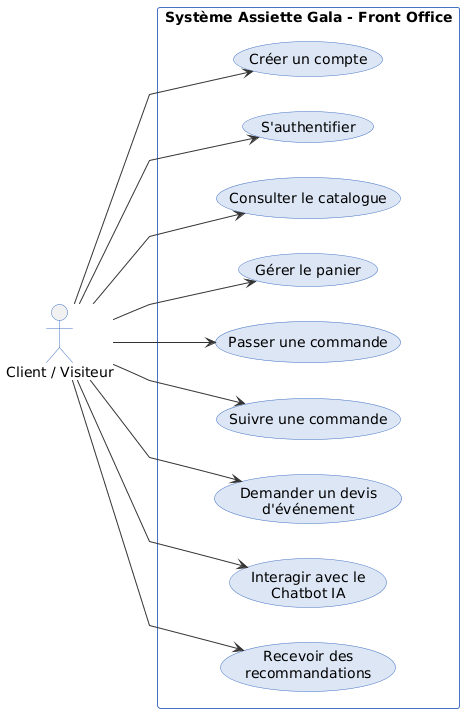
\includegraphics[width=0.95\textwidth,height=0.72\textheight,keepaspectratio]{uc_global_front.png}
    \caption{Cas d'utilisation global : Front Office}
    \label{fig:uc_global_front}
\end{figure}

\begin{figure}[!htbp]
    \centering
    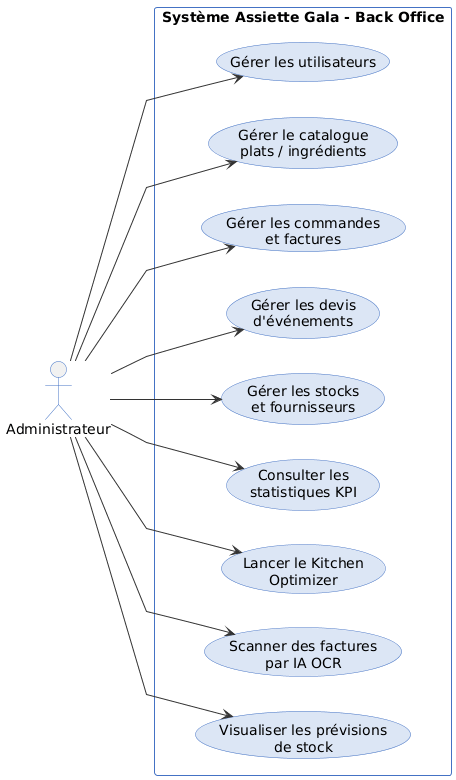
\includegraphics[width=0.95\textwidth,height=0.72\textheight,keepaspectratio]{uc_global_back.png}
    \caption{Cas d'utilisation global : Back Office}
    \label{fig:uc_global_back}
\end{figure}

% --------------------------------------------------
\section{Diagramme de classes global}

La Figure~\ref{fig:class_global} présente la structure statique de la solution, en mettant en lumière les entités métier, leurs attributs et les relations entre services.

\begin{figure}[H]
    \centering
    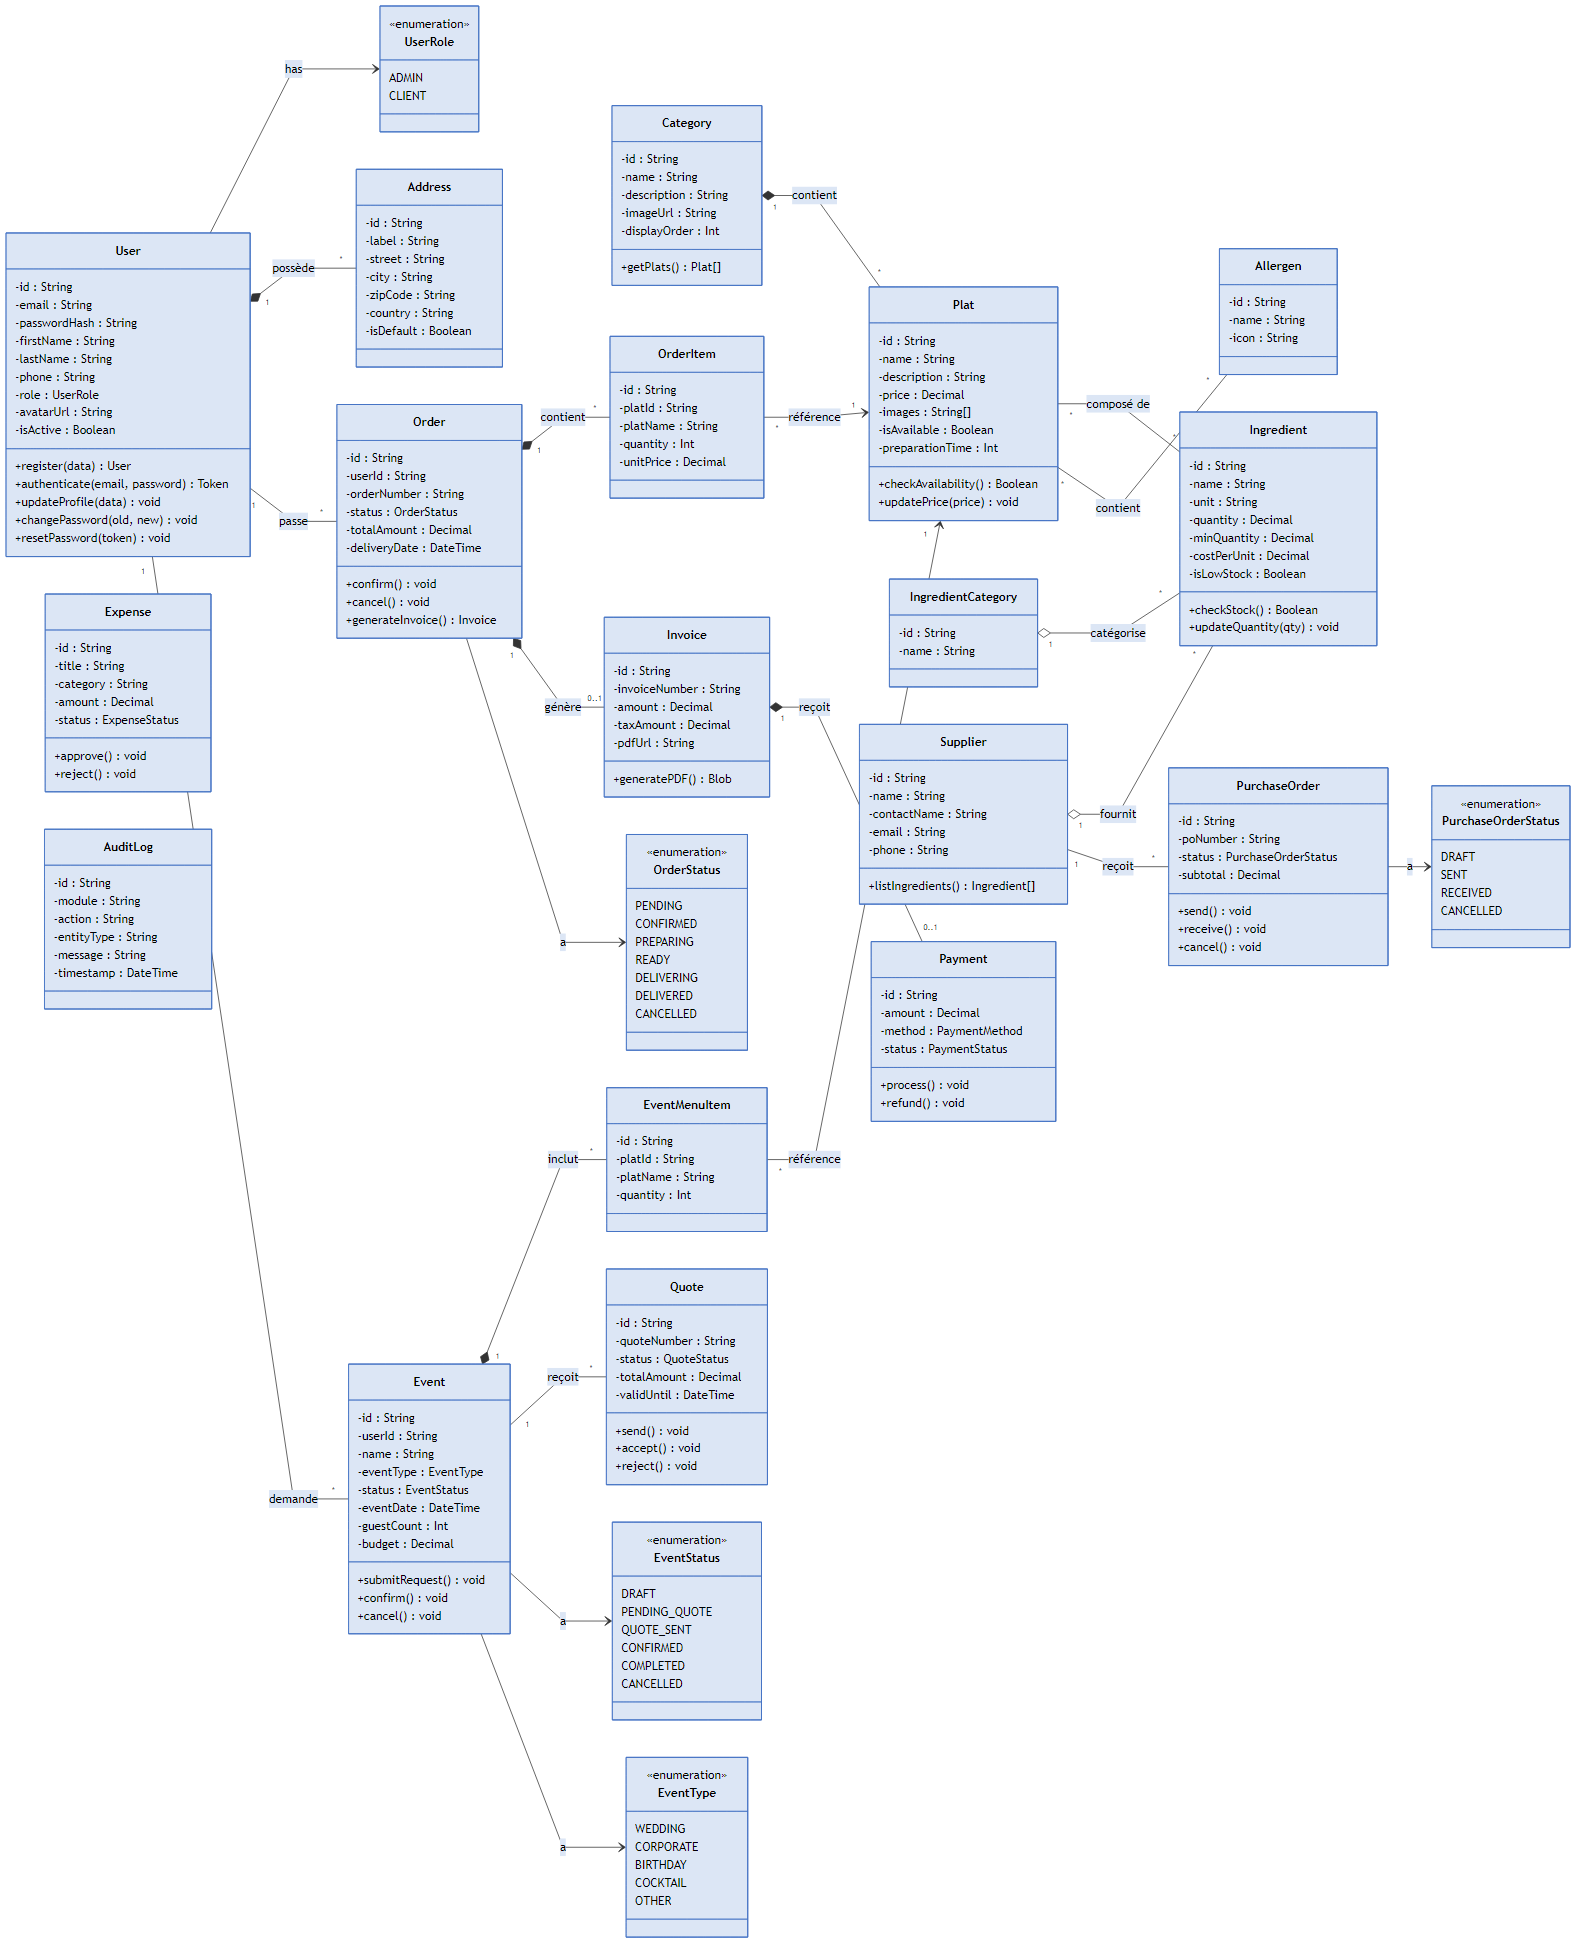
\includegraphics[width=0.95\textwidth]{class_global.png}
    \caption{Diagramme de classes global du système}
    \label{fig:class_global}
\end{figure}

% --------------------------------------------------
% --------------------------------------------------
\section*{Conclusion}
\addcontentsline{toc}{section}{Conclusion}

\begin{samepage}
Ce chapitre liminaire a posé le socle de notre intervention. En radiographiant les carences des solutions du marché et en les confrontant aux exigences réelles d'Assiette Gala Sfaxienne, nous avons justifié la conception d'un portail intégralement sur mesure. Le cadre Scrum et la notation UML baliseront la route des six sprints à venir. Le chapitre suivant détaille l'architecture logicielle et l'environnement technique retenus pour matérialiser cette vision.
\end{samepage}



% Chapitre 2 : Architecture logicielle et framework de développement (bleu)
\clearpage
\renewcommand{\currentchapcolor}{chap-archi}
% ============================================================
% CHAPITRE 2 : ARCHITECTURE LOGICIELLE ET FRAMEWORK DE DÉVELOPPEMENT
% ============================================================
\chapter{Architecture logicielle et framework de développement}

\section{Introduction}

Avant de plonger dans la réalisation des sprints, il est indispensable de présenter les fondations techniques sur lesquelles repose l'ensemble de la solution. Ce chapitre détaille l'environnement matériel et logiciel mobilisé, l'architecture de déploiement retenue ainsi que l'organisation interne des microservices et de leurs interconnexions.

% --------------------------------------------------
\section{Environnement de développement}

\subsection{Environnement matériel}

\begin{table}[H]
    \centering
    \caption{Poste de travail utilisé}
    \label{tab:env_materiel}
    \begin{tabular}{|l|l|}
        \hline
        \textbf{Composant} & \textbf{Spécification} \\
        \hline
        Machine & PC portable Lenovo \\
        \hline
        Processeur & Intel Core i7 13650HX \\
        \hline
        Mémoire vive & 16 Go RAM \\
        \hline
        Stockage & SSD 512 Go \\
        \hline
        Système d'exploitation & Windows 11  \\
        \hline
    \end{tabular}
\end{table}

\subsection{Environnement logiciel}

Le Tableau~\ref{tab:env_logiciel} recense les outils mobilisés.

\begin{table}[H]
    \centering
    \caption{Outils et technologies du projet}
    \label{tab:env_logiciel}
    \renewcommand{\arraystretch}{1.3}
    \begin{tabular}{|p{3.5cm}|p{3cm}|p{6cm}|}
        \hline
        \textbf{Outil / Technologie} & \textbf{Version} & \textbf{Rôle dans le projet} \\
        \hline
        Visual Studio Code & Dernière & Environnement de rédaction du code \\
        \hline
        Node.js & 20+ & Moteur d'exécution des microservices \\
        \hline
        TypeScript & 5.x & Couche de typage pour fiabiliser les échanges \\
        \hline
        React & 19 & Construction des écrans (client et admin) \\
        \hline
        Vite & 7.x & Compilation ultra-rapide du Frontend \\
        \hline
        Tailwind CSS & 4.x & Habillage graphique via classes utilitaires \\
        \hline
        Express.js & 4.x & Routage HTTP interne des API \\
        \hline
        Prisma ORM & 5.x & Pont de communication avec PostgreSQL \\
        \hline
        PostgreSQL & 16 & Stockage des menus, utilisateurs et commandes \\
        \hline
        Python & 3.14 & Scripts d'intelligence artificielle \\
        \hline
        FastAPI & Dernière & Interface rapide pour le chatbot \\
        \hline
        LangChain & 0.3.x & Orchestrateur des requêtes RAG \\
        \hline
        Google Gemini & 2.5 Flash & Modèle linguistique générant les réponses \\
        \hline
        Figma & En ligne & Maquettage graphique \\
        \hline
        Git & Dernière & Versionnement du code source \\
        \hline
        Postman & Dernière & Simulation et validation des requêtes API \\
        \hline
        Cloudinary & Cloud & Hébergement externe des photos de plats \\
        \hline
        FAISS (faiss-cpu) & 1.7+ & Index vectoriel pour le pipeline RAG \\
        \hline
    \end{tabular}
\end{table}

% --------------------------------------------------
\section{Architecture de déploiement}

Le diagramme de déploiement (figure~\ref{fig:deploiement}) détaille la distribution physique des composants logiciels de la plateforme Assiette Gala, en illustrant les nœuds d'exécution (poste client, serveur d'application, serveur de bases de données) et les services externes mobilisés (Cloudinary, Google Gemini, Flouci, SMTP).

\begin{figure}[H]
    \centering
    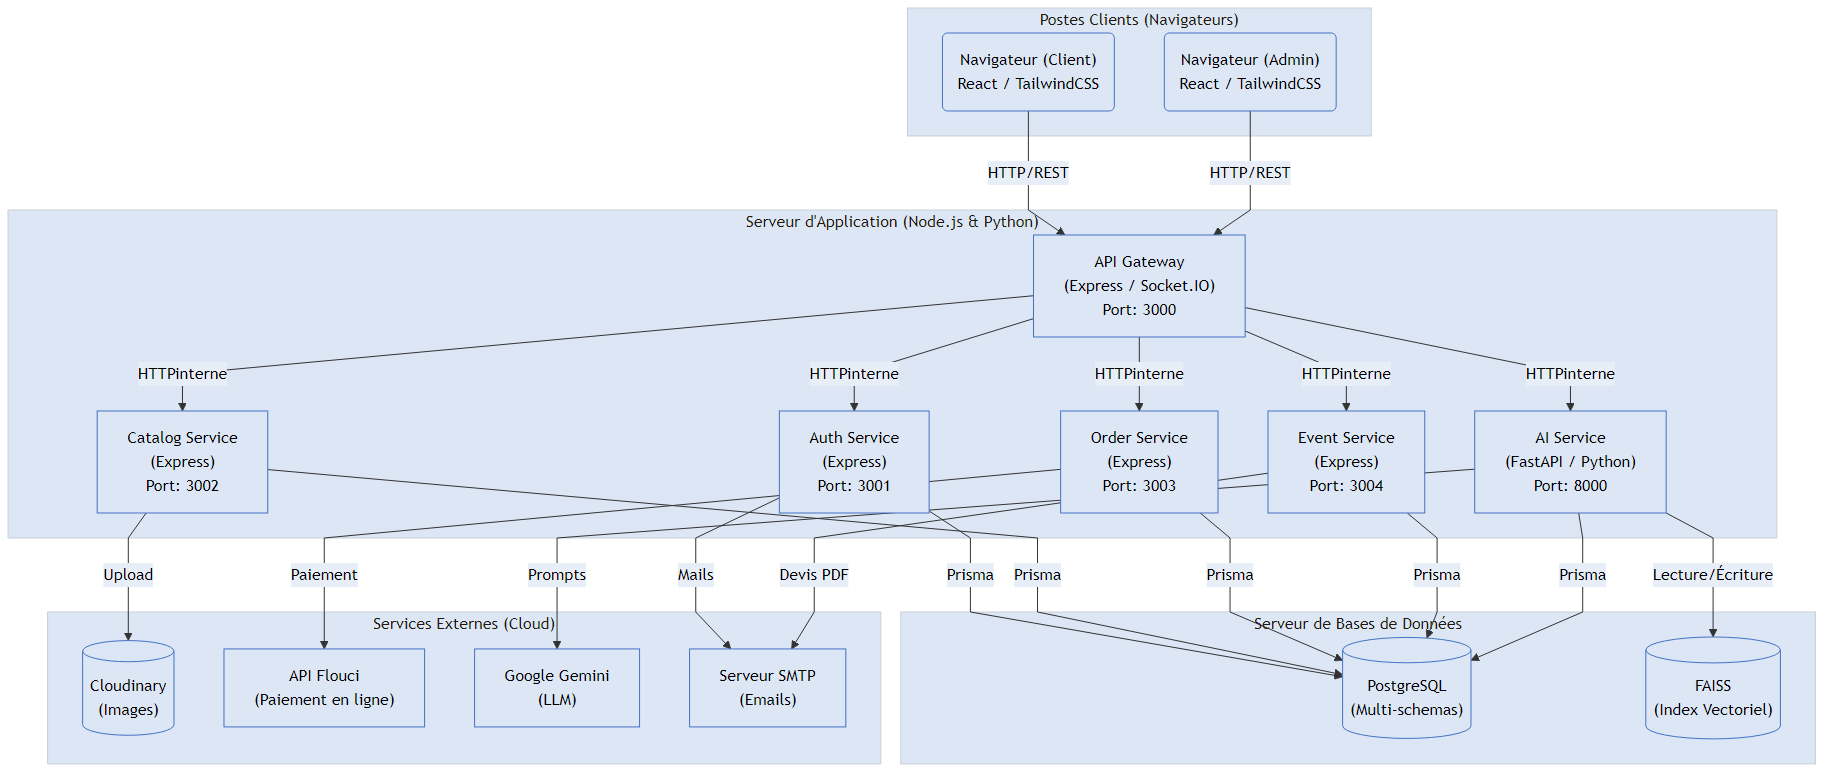
\includegraphics[width=0.95\textwidth]{deploiement.png}
    \caption{Diagramme de déploiement de la plateforme Assiette Gala}
    \label{fig:deploiement}
\end{figure}

La figure~\ref{fig:architecture_globale} offre une vue d'ensemble de l'architecture logicielle de la plateforme, mettant en évidence les flux de communication entre le frontend, la passerelle API, les microservices métier, le service IA et les bases de données.

\begin{figure}[H]
    \centering
    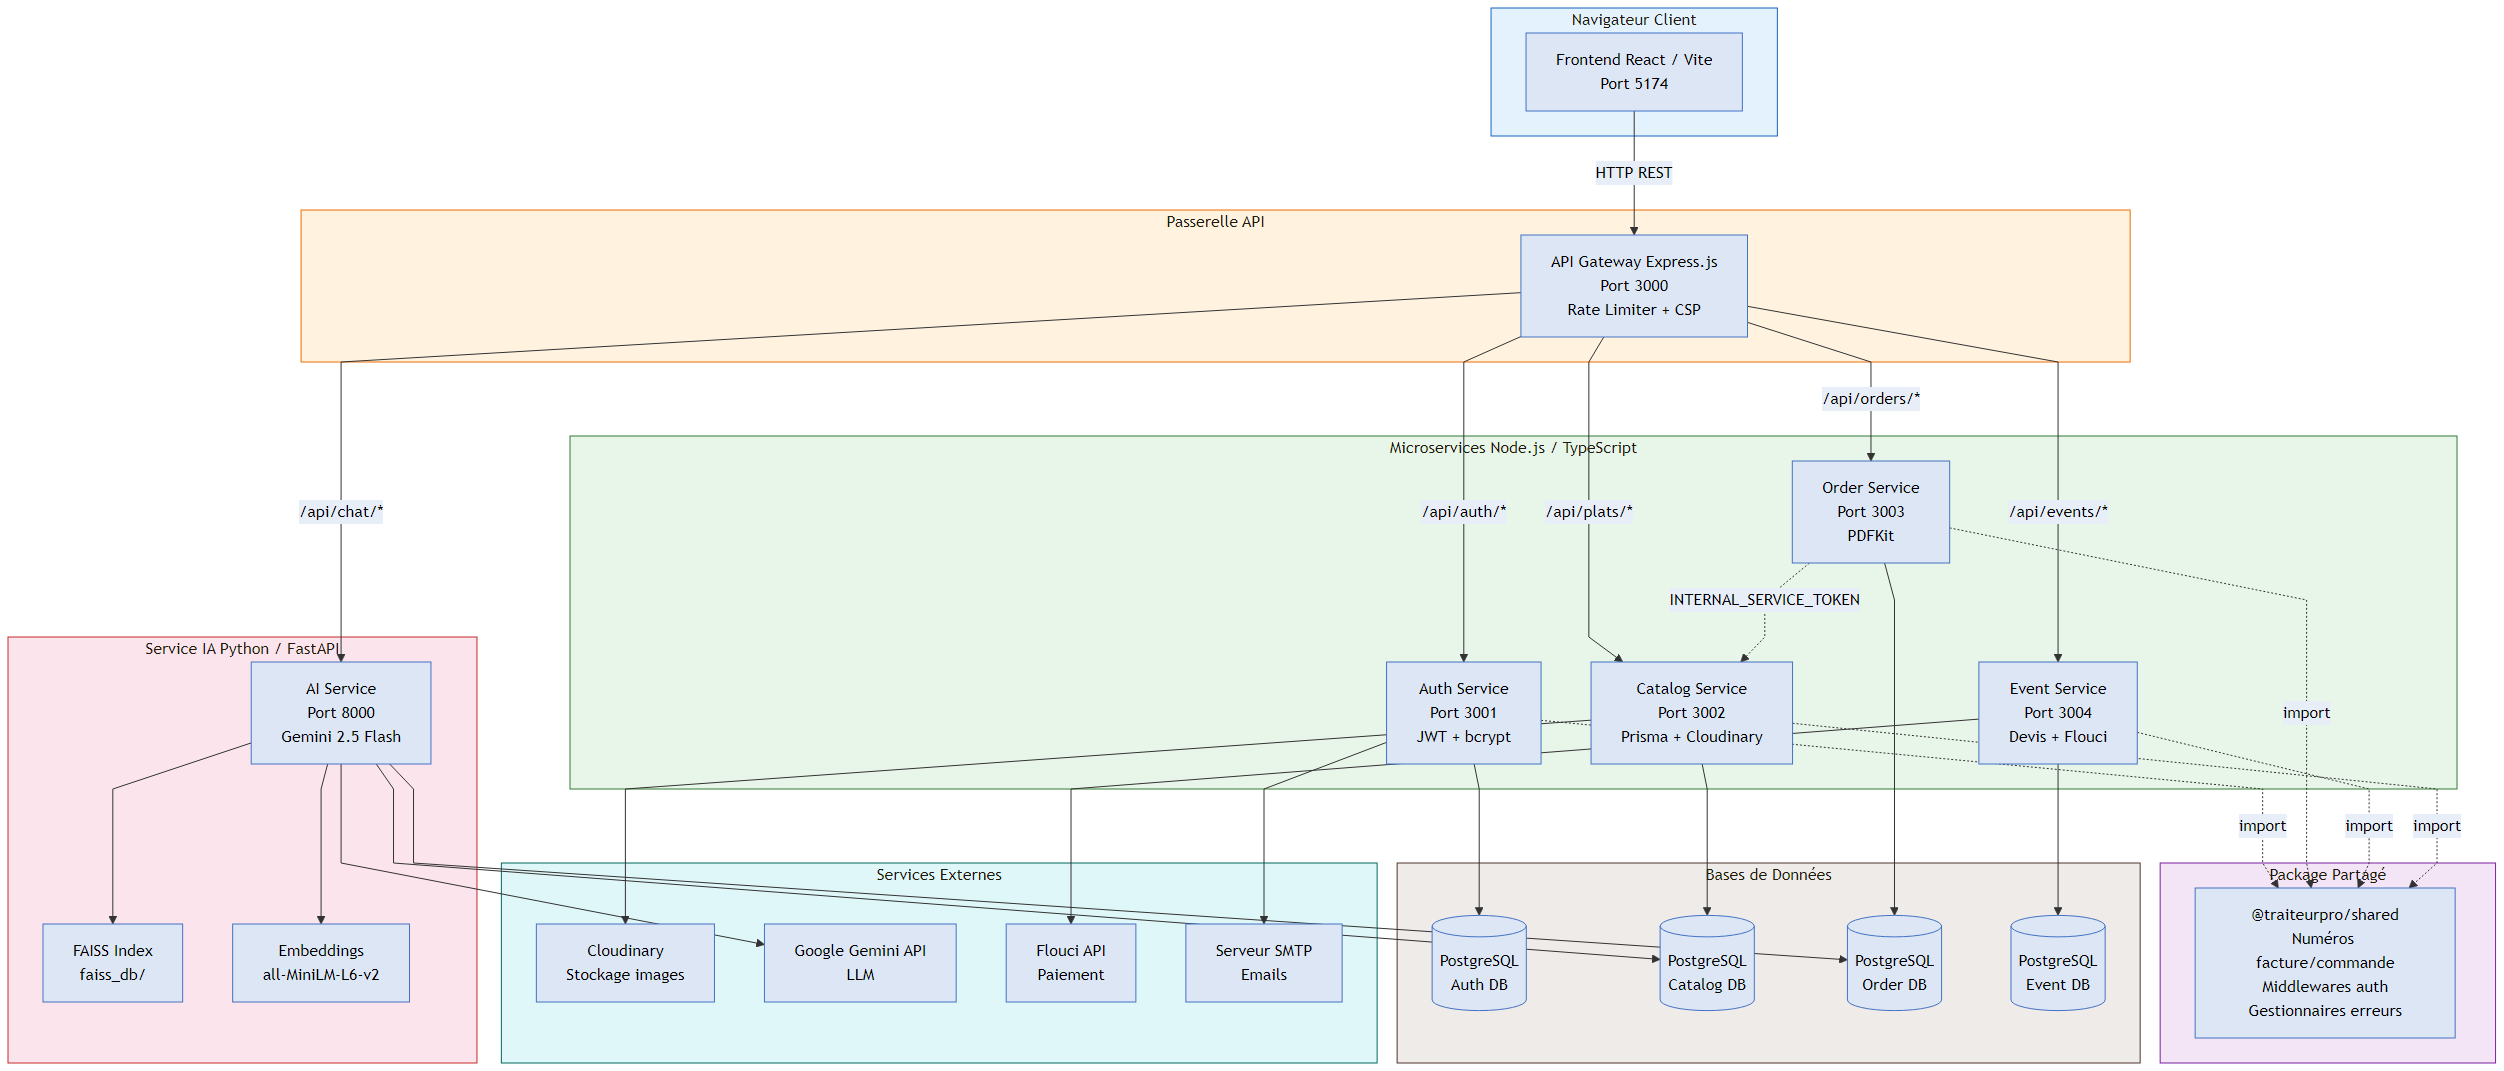
\includegraphics[width=0.95\textwidth]{architecture_globale.png}
    \caption{Architecture globale de la plateforme Assiette Gala}
    \label{fig:architecture_globale}
\end{figure}

% --------------------------------------------------
\section{Architecture technique détaillée}

\subsection{Découpage en microservices}

La solution Assiette Gala se compose de sept briques logicielles autonomes, chacune spécialisée dans un domaine métier :

\begin{table}[H]
    \centering
    \caption{Microservices de la plateforme Assiette Gala}
    \label{tab:microservices}
    \renewcommand{\arraystretch}{1.3}
    \begin{tabular}{|p{3.5cm}|c|p{6cm}|}
        \hline
        \textbf{Service} & \textbf{Port} & \textbf{Responsabilité} \\
        \hline
        API Gateway & 3000 & Point d'entrée unique, routage, authentification, WebSocket \\
        \hline
        Auth Service & 3001 & Inscription, connexion, JWT, Google OAuth, profils \\
        \hline
        Catalog Service & 3002 & Plats, catégories, allergènes, stock, fournisseurs \\
        \hline
        Order Service & 3003 & Commandes, paiements, factures PDF \\
        \hline
        Event Service & 3004 & Événements, devis, modèles de réception \\
        \hline
        AI Service & 8000 & Chatbot RAG, recommandations, prévisions, cuisine \\
        \hline
        Frontend (Vite) & 5174 & Interface React (client et administration) \\
        \hline
    \end{tabular}
\end{table}

\subsection{Passerelle d'entrée (API Gateway)}

Pour éviter que le navigateur du client n'ait à connaître l'adresse de sept serveurs distincts, une \textbf{passerelle unique} (port 3000) joue le rôle de standard téléphonique : elle réceptionne chaque appel HTTP, vérifie le badge JWT du demandeur, puis achemine la requête vers la bonne cuisine logicielle.

\subsection{Package partagé (\texttt{@traiteurpro/shared})}

Afin d'éliminer la duplication de code entre les microservices, un package npm interne centralise les utilitaires communs :

\begin{itemize}
    \item \textbf{Middleware d'authentification :} vérification JWT, extraction du rôle utilisateur.
    \item \textbf{Gestionnaire d'erreurs :} format de réponse uniforme pour toutes les API.
    \item \textbf{Utilitaires de facturation :} génération des numéros de facture (format \texttt{INV-YYYYMM-<hex>}) et de commande (format \texttt{ORD-YYMMDD-<hex>}).
    \item \textbf{Types partagés :} interfaces TypeScript pour les entités transversales (utilisateur, commande, plat).
    \item \textbf{Validations :} schémas Zod pour la validation des entrées.
\end{itemize}

\subsection{Communication inter-services}

Les microservices communiquent entre eux via des appels HTTP internes sécurisés par un \textbf{jeton de service interne} (\texttt{INTERNAL\_SERVICE\_TOKEN}). Ce jeton, partagé exclusivement entre les services backend, empêche tout accès non autorisé aux endpoints internes.

Pour les notifications en temps réel, la passerelle API expose un serveur \textbf{WebSocket} (Socket.IO) qui diffuse les événements (nouvelle commande, mise à jour de statut) vers les clients connectés.

% --------------------------------------------------
\section*{Conclusion}
\addcontentsline{toc}{section}{Conclusion}

\begin{samepage}
Ce chapitre a dressé le panorama complet de l'outillage et de l'architecture technique de la plateforme Assiette Gala. Le découpage en microservices, la centralisation des utilitaires via le package partagé et la passerelle d'entrée unique garantissent une base solide pour les six sprints à venir. Le chapitre suivant inaugure le premier cycle de développement : la mise en place du système d'authentification.
\end{samepage}



% Chapitre 3 (Sprint 1) : Gestion des utilisateurs (vert)
\clearpage
\renewcommand{\currentchapcolor}{chap-auth}
% ============================================================
% CHAPITRE 3 (Sprint 1)
% ============================================================
\chapter{Sprint 1 : Gestion des utilisateurs}

\section{Introduction}

Dès l'entame du projet, ce premier cycle de développement s'est penché sur l'architecture de sécurité d'Assiette Gala. Il était indispensable d'isoler l'interface grand public de l'interface secrète d'administration. En s'appuyant sur les recommandations de M. Omar Daoud, nous avons créé une muraille virtuelle où chaque visiteur, client ou cuisinier dispose d'autorisations cloisonnées (JWT). Ce volet retrace la mise sur pied de ce rempart d'identité.

% --------------------------------------------------
\section{Backlog du sprint}

Le tableau~\ref{tab:backlog_sprint1} reprend les user stories attribuées au sprint~1.

\begin{table}[H]
    \centering
    \caption{Backlog du sprint 1}
    \label{tab:backlog_sprint1}
    \renewcommand{\arraystretch}{1.3}
    \begin{tabular}{|c|p{8cm}|c|}
        \hline
        \textbf{ID} & \textbf{User Story} & \textbf{Durée} \\
        \hline
        US-01 & En tant que visiteur, je souhaite créer un compte afin d'accéder aux fonctionnalités. & 5 \\
        \hline
        US-02 & En tant qu'utilisateur, je souhaite me connecter avec mes identifiants. & 3 \\
        \hline
        US-03 & En tant qu'utilisateur, je souhaite me connecter via Google OAuth. & 5 \\
        \hline
        US-04 & En tant qu'utilisateur, je souhaite réinitialiser mon mot de passe. & 3 \\
        \hline
        US-05 & En tant qu'utilisateur, je souhaite modifier mes informations personnelles. & 2 \\
        \hline
        US-06 & En tant qu'administrateur, je souhaite gérer les comptes utilisateurs. & 5 \\
        \hline
    \end{tabular}
\end{table}

% --------------------------------------------------
\section{Conception}

\subsection{Diagramme de cas d'utilisation}

Le diagramme de cas d'utilisation du sprint~1 (figure~\ref{fig:uc_sprint1}) détaille les interactions des acteurs avec le module d'authentification.

\begin{figure}[H]
    \centering
    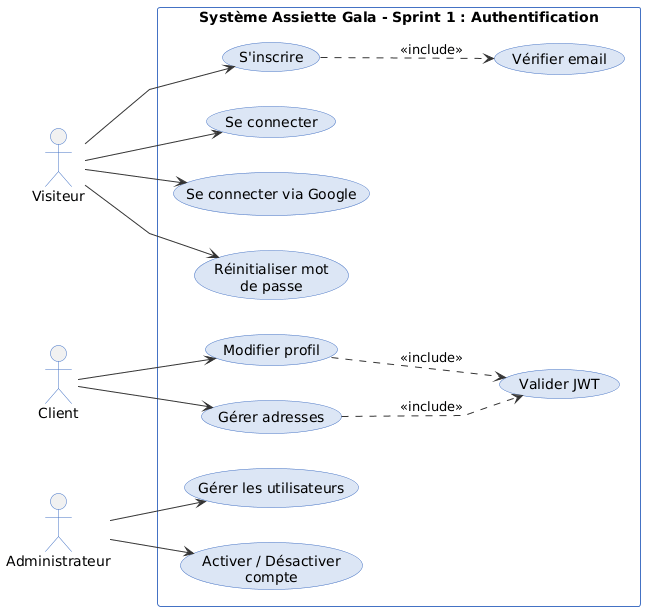
\includegraphics[width=0.85\textwidth]{uc_sprint1.png}
    \caption{Diagramme de cas d'utilisation du sprint 1}
    \label{fig:uc_sprint1}
\end{figure}

\subsection{Description textuelle des cas d'utilisation}

\subsubsection{Cas d'utilisation : Inscription}

\begin{table}[H]
    \centering
    \caption{Description textuelle : Inscription}
    \label{tab:desc_inscription}
    \renewcommand{\arraystretch}{1.3}
    \begin{tabular}{|p{4cm}|p{8.5cm}|}
        \hline
        \textbf{Cas d'utilisation} & Inscription \\
        \hline
        \textbf{Acteur principal} & Visiteur \\
        \hline
        \textbf{Précondition} & Le visiteur n'est pas authentifié \\
        \hline
        \textbf{Postcondition} & Un compte utilisateur est créé avec le rôle CLIENT \\
        \hline
        \textbf{Scénario principal} &
        \begin{enumerate}
            \item Le badaud navigue vers le portail de création de compte Gala
            \item Le formulaire récolte ses coordonnées (téléphone, courriel, nom complet)
            \item Le backend s'assure qu'aucun autre compte n'exploite cet email
            \item Application du chiffrement Bcrypt sur le mot de passe brut
            \item Injection du dossier dans la base de données puis émission d'un mail de blocage
            \item Clic sur le jeton de libération reçu par messagerie
            \item Le compte traiteur est opérationnel
        \end{enumerate} \\
        \hline
        \textbf{Scénario alternatif} &
        \begin{itemize}
            \item[3a.] Doublon du courriel : blocage direct sur l'interface
            \item[2a.] Données partielles : impossibilité de valider l'action
        \end{itemize} \\
        \hline
    \end{tabular}
\end{table}

\subsubsection{Cas d'utilisation : Connexion}

\begin{table}[H]
    \centering
    \caption{Description textuelle : Connexion}
    \label{tab:desc_connexion}
    \renewcommand{\arraystretch}{1.3}
    \begin{tabular}{|p{4cm}|p{8.5cm}|}
        \hline
        \textbf{Cas d'utilisation} & Connexion \\
        \hline
        \textbf{Acteur principal} & Utilisateur (Client ou Administrateur) \\
        \hline
        \textbf{Précondition} & L'utilisateur possède un compte activé \\
        \hline
        \textbf{Postcondition} & L'utilisateur est authentifié et reçoit un jeton JWT \\
        \hline
        \textbf{Scénario principal} &
        \begin{enumerate}
            \item Positionnement sur la mire d'identification
            \item Frappe des clés d'accès personnelles
            \item Interrogation de la base de données PostgreSQL
            \item Comparaison mathématique avec l'empreinte bcrypt stockée
            \item Délivrance d'un passeport temporaire (15 min) et d'un visa de fond (7 jours)
            \item Orientation automatique vers l'espace de commande
        \end{enumerate} \\
        \hline
        \textbf{Scénario alternatif} &
        \begin{itemize}
            \item[3a.] Email fantôme : rejet muet (pour éviter les fuites d'info)
            \item[4a.] Erreur de mot de passe : rejet explicite
            \item[3b.] Email en attente de validation : consigne d'ouverture de messagerie
        \end{itemize} \\
        \hline
    \end{tabular}
\end{table}

\subsubsection{Cas d'utilisation : Réinitialisation du mot de passe}

\begin{table}[H]
    \centering
    \caption{Description textuelle : Réinitialisation du mot de passe}
    \label{tab:desc_reset_password}
    \renewcommand{\arraystretch}{1.3}
    \begin{tabular}{|p{4cm}|p{8.5cm}|}
        \hline
        \textbf{Cas d'utilisation} & Réinitialiser le mot de passe \\
        \hline
        \textbf{Acteur principal} & Utilisateur \\
        \hline
        \textbf{Précondition} & L'utilisateur possède un compte enregistré \\
        \hline
        \textbf{Postcondition} & Le mot de passe est remplacé par un nouveau mot de passe haché \\
        \hline
        \textbf{Scénario principal} &
        \begin{enumerate}
            \item Appui sur l'alerte d'oubli de clés
            \item Désignation de son adresse de secours
            \item Forgeage d'un token aléatoire jetable
            \item Livraison d'un lien encapsulé vers l'adresse indiquée
            \item Activation du lien et proposition d'une nouvelle combinaison secrète
            \item Le serveur écrase l'ancienne empreinte bcrypt par la nouvelle
        \end{enumerate} \\
        \hline
        \textbf{Scénario alternatif} &
        \begin{itemize}
            \item[4a.] Jetons obsolètes : obligation de recommencer la démarche
        \end{itemize} \\
        \hline
    \end{tabular}
\end{table}

\subsection{Diagrammes de séquence}

\subsubsection{Séquence : Inscription}

\begin{figure}[H]
    \centering
    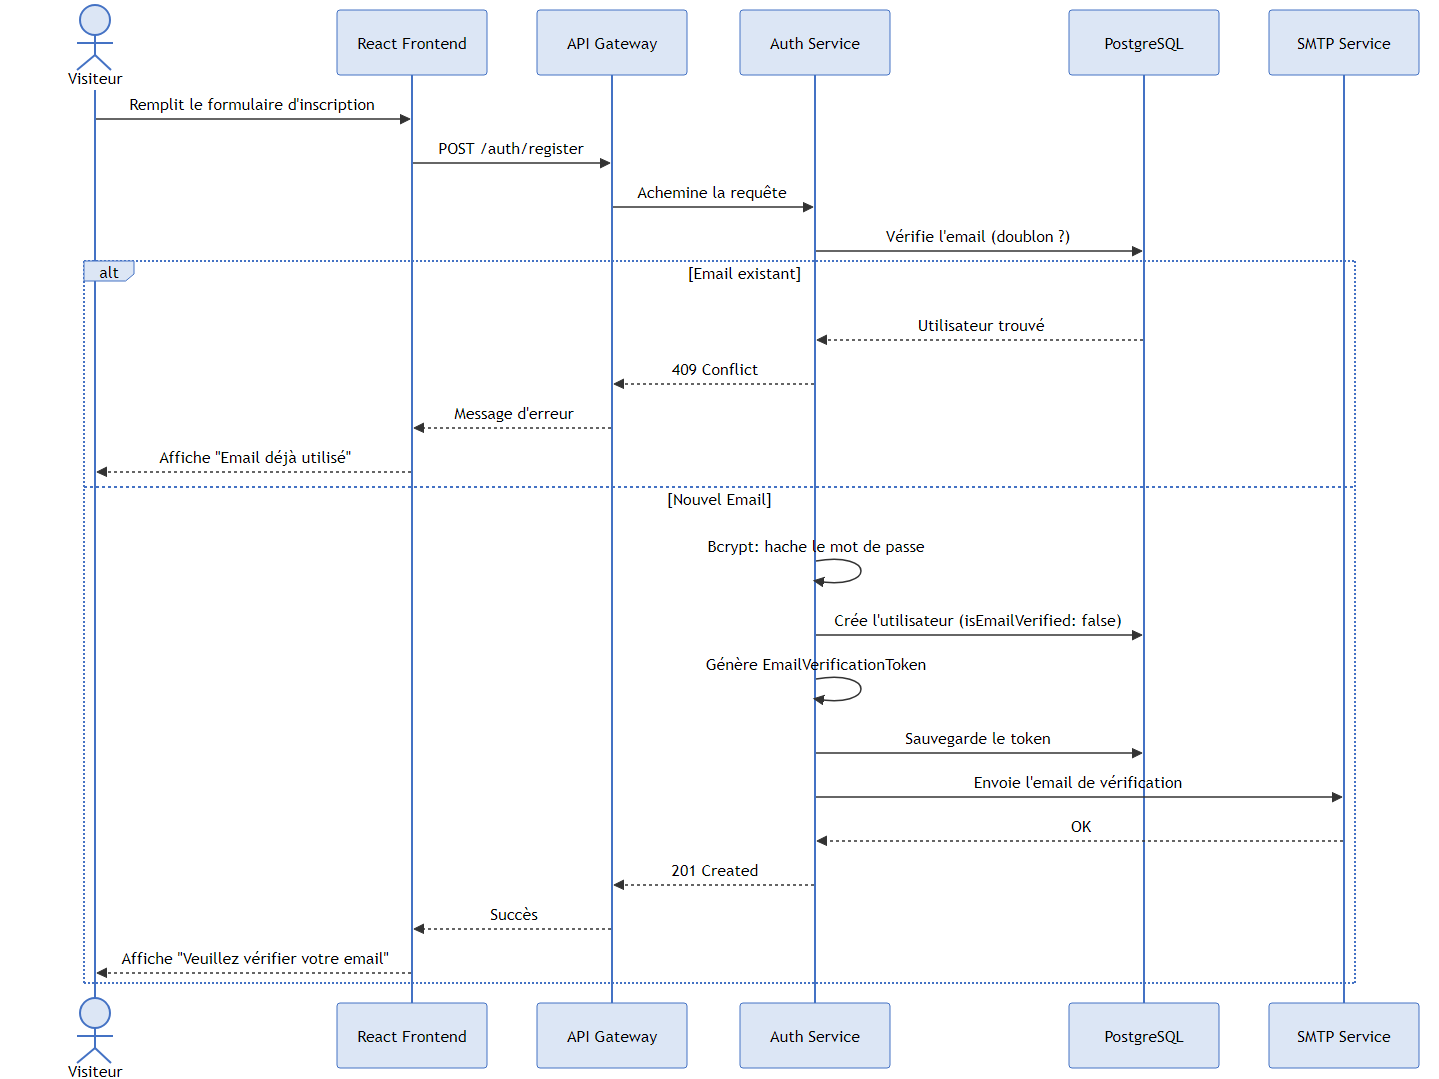
\includegraphics[width=0.9\textwidth]{seq_inscription.png}
    \caption{Diagramme de séquence : Inscription}
    \label{fig:seq_inscription}
\end{figure}

\subsubsection{Séquence : Connexion}

\begin{figure}[H]
    \centering
    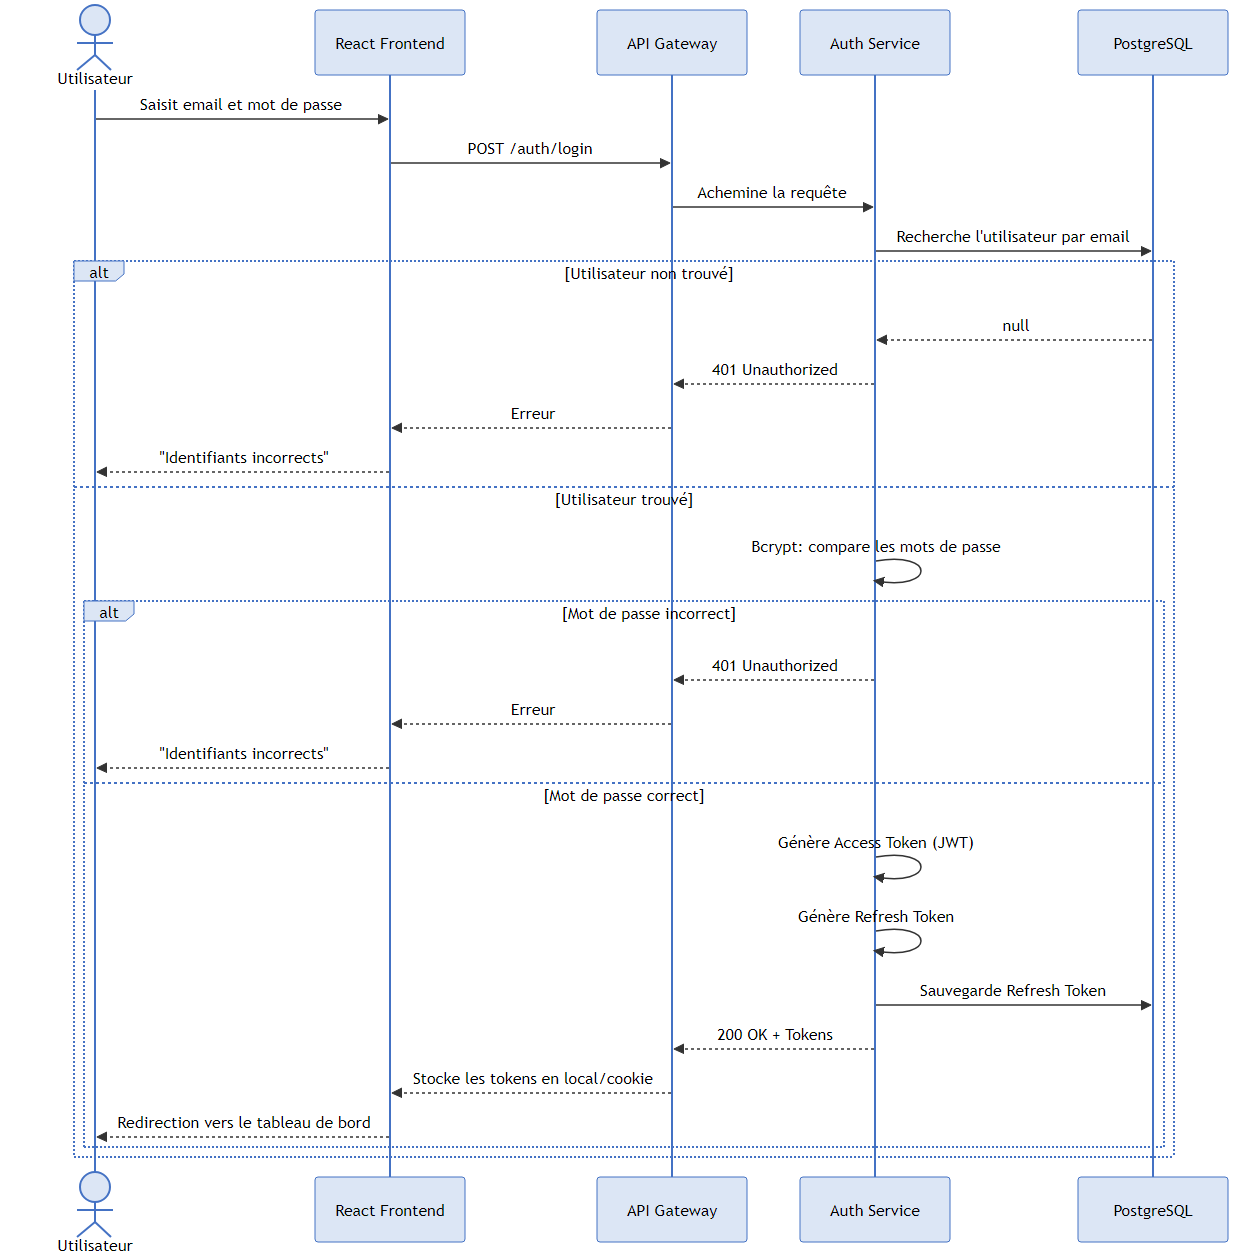
\includegraphics[width=0.9\textwidth]{seq_connexion.png}
    \caption{Diagramme de séquence : Connexion}
    \label{fig:seq_connexion}
\end{figure}

\subsubsection{Séquence : Réinitialisation du mot de passe}

\begin{figure}[H]
    \centering
    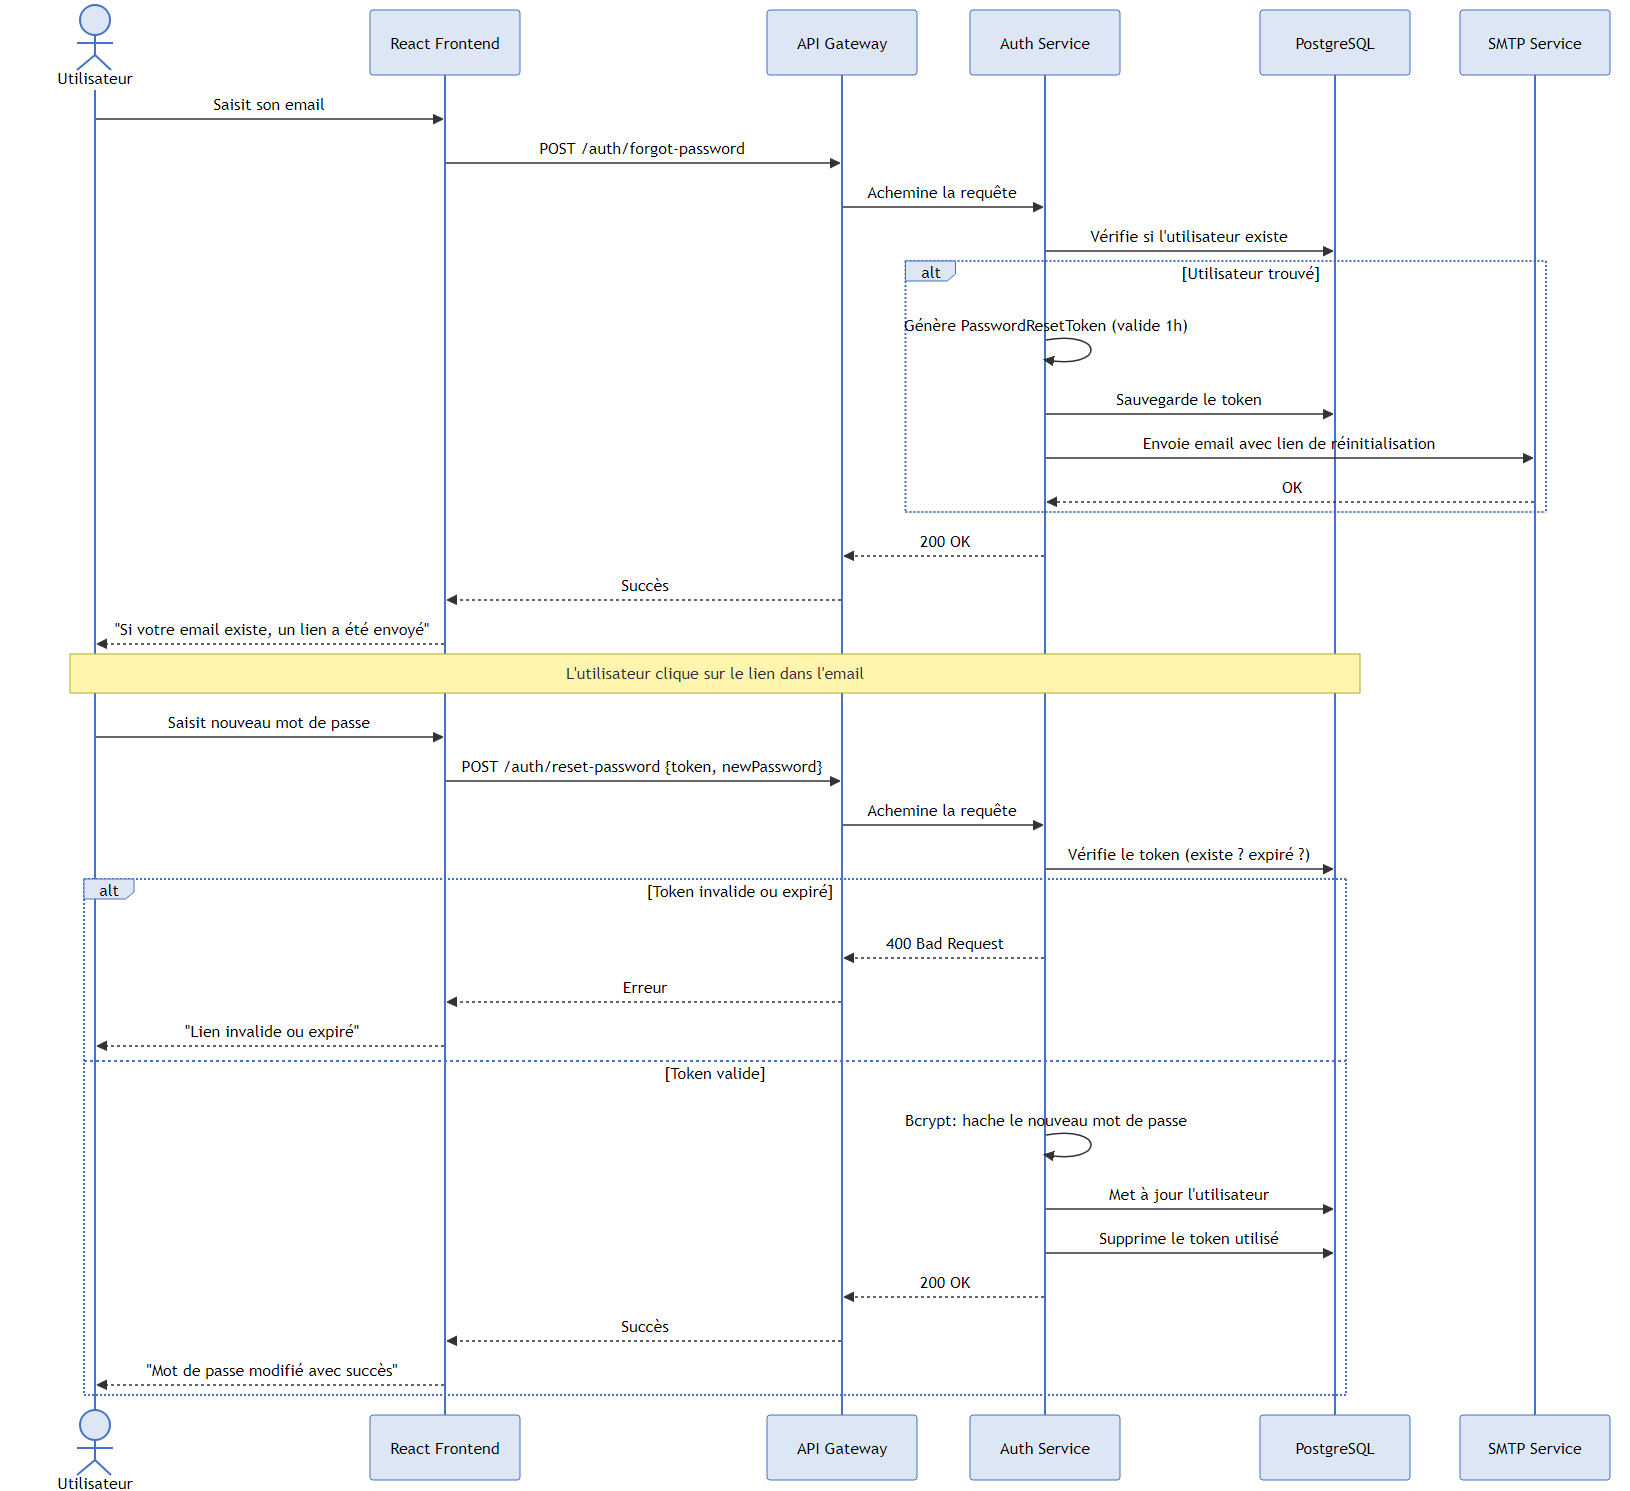
\includegraphics[width=0.9\textwidth]{seq_reset_password.png}
    \caption{Diagramme de séquence : Réinitialisation du mot de passe}
    \label{fig:seq_reset_password}
\end{figure}

\subsection{Diagramme de classes}

Le diagramme de classes (figure~\ref{fig:class_sprint1}) modélise les entités manipulées par le service d'authentification. Le modèle central \texttt{User} comporte les attributs nécessaires à l'identification, la sécurité et la gestion du profil. L'entité \texttt{Address} associe une ou plusieurs adresses de livraison à chaque utilisateur.

\begin{figure}[H]
    \centering
    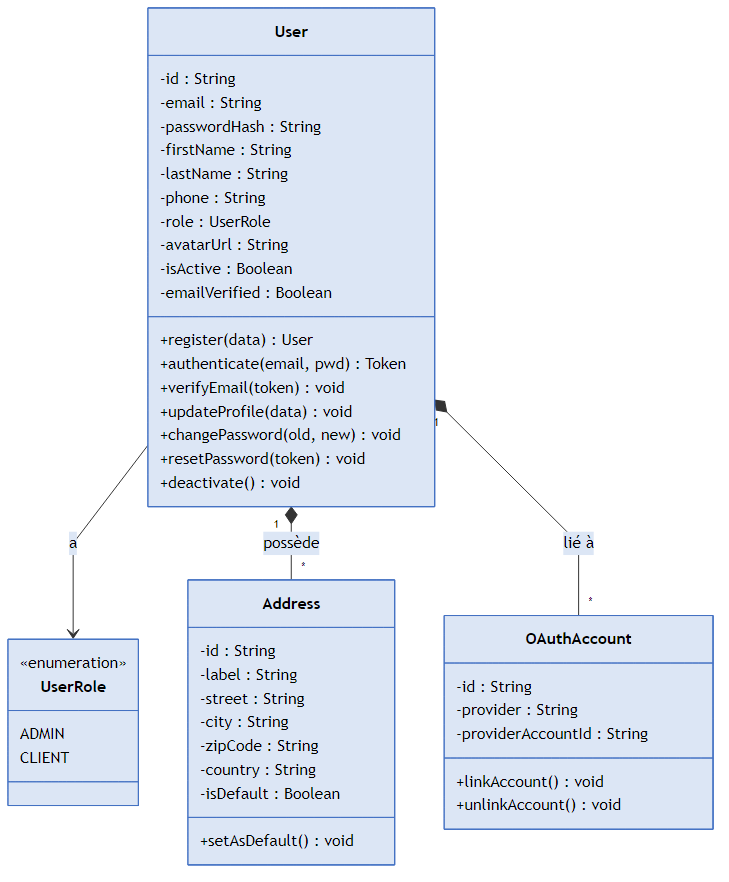
\includegraphics[width=0.85\textwidth]{class_sprint1.png}
    \caption{Diagramme de classes du service d'authentification}
    \label{fig:class_sprint1}
\end{figure}

Le modèle \texttt{User} contient les attributs suivants :
\begin{itemize}
    \item \texttt{id} : identifiant unique (UUID généré automatiquement)
    \item \texttt{firstName}, \texttt{lastName} : nom et prénom
    \item \texttt{email} : adresse email (unique, indexée)
    \item \texttt{password} : mot de passe haché (bcrypt, 10 rounds)
    \item \texttt{phone} : numéro de téléphone (optionnel)
    \item \texttt{role} : énumération (\texttt{CLIENT}, \texttt{ADMIN})
    \item \texttt{isVerified} : indicateur de vérification de l'email
    \item \texttt{googleId} : identifiant Google pour OAuth 2.0 (optionnel)
    \item \texttt{avatar} : URL de la photo de profil (optionnel)
    \item \texttt{resetToken}, \texttt{resetTokenExpiry} : jeton et date d'expiration pour la réinitialisation du mot de passe
\end{itemize}

Le modèle \texttt{Address} contient :
\begin{itemize}
    \item \texttt{id} : identifiant unique
    \item \texttt{label} : libellé de l'adresse (ex. : <<~Domicile~>>, <<~Bureau~>>)
    \item \texttt{street}, \texttt{city}, \texttt{postalCode} : composantes de l'adresse
    \item \texttt{isDefault} : indicateur de l'adresse par défaut
    \item \texttt{userId} : clé étrangère vers \texttt{User}
\end{itemize}

\subsection{Diagramme d'états-transitions}

Le diagramme d'états-transitions (figure~\ref{fig:state_sprint1}) illustre le cycle de vie d'un compte utilisateur au sein de la plateforme Assiette Gala, depuis sa création jusqu'à sa suppression éventuelle.

\begin{figure}[H]
    \centering
    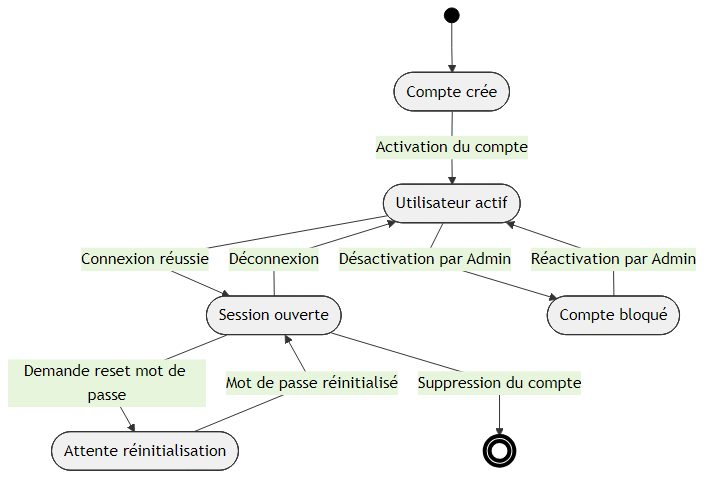
\includegraphics[width=0.85\textwidth]{state_sprint1_user.png}
    \caption{Diagramme d'états-transitions : Cycle de vie d'un utilisateur}
    \label{fig:state_sprint1}
\end{figure}

% --------------------------------------------------
\section{Réalisation}

\subsection{Structure du service}

Le microservice d'identité d'Assiette Gala obéit à un empilement en quatre strates :

\begin{itemize}
    \item \textbf{Portes d'entrée} (\texttt{auth.routes.ts}) : cartographie des chemins HTTP acceptés par le service.
    \item \textbf{Écluses} (\texttt{auth.controller.ts}) : désossage de chaque requête, aiguillage vers la couche métier.
    \item \textbf{Réacteur métier} (\texttt{auth.service.ts}) : contrôle des règles (hachage bcrypt, forgerie de jetons, envoi de courriels).
    \item \textbf{Empreinte Prisma} (\texttt{schema.prisma}) : moulage des tables PostgreSQL.
    \item \textbf{Vigiles} (middlewares) : interception du badge JWT avant toute opération sensible. Le middleware d'administration est autonome et vérifie lui-même le jeton si nécessaire.
    \item \textbf{Boîte à outils commune} (\texttt{shared}) : package npm partagé entre tous les microservices, regroupant les utilitaires de facturation (génération des numéros de facture et de commande), les middlewares d'authentification et les gestionnaires d'erreurs.
\end{itemize}

\subsection{Points d'entrée de l'API}

\begin{table}[H]
    \centering
    \caption{Endpoints REST du service d'authentification}
    \label{tab:endpoints_auth}
    \renewcommand{\arraystretch}{1.2}
    \begin{tabular}{|l|p{4.5cm}|p{5.5cm}|}
        \hline
        \textbf{Méthode} & \textbf{Route} & \textbf{Description} \\
        \hline
        POST & /api/auth/register & Inscription d'un nouvel utilisateur \\
        \hline
        POST & /api/auth/login & Connexion par identifiants \\
        \hline
        POST & /api/auth/google & Authentification via Google \\
        \hline
        POST & /api/auth/forgot-password & Demande de réinitialisation \\
        \hline
        POST & /api/auth/reset-password & Réinitialisation du mot de passe \\
        \hline
        GET & /api/auth/verify-email/:token & Vérification de l'email \\
        \hline
        POST & /api/auth/refresh-token & Rafraîchissement du jeton \\
        \hline
        GET & /api/auth/profile & Consultation du profil \\
        \hline
        PUT & /api/auth/profile & Modification du profil \\
        \hline
        GET & /api/auth/addresses & Liste des adresses \\
        \hline
        POST & /api/auth/addresses & Ajout d'une adresse \\
        \hline
        PUT & /api/auth/addresses/:id & Modification d'une adresse \\
        \hline
        DELETE & /api/auth/addresses/:id & Suppression d'une adresse \\
        \hline
        GET & /api/auth/admin/users & Liste des utilisateurs (administrateur) \\
        \hline
    \end{tabular}
\end{table}

% Schéma de la base de données retiré : le diagramme de classes (figure~\ref{fig:class_sprint1}) suffit à modéliser la structure des données.


\subsection{Mécanisme d'authentification JWT}

Le dispositif d'identification du traiteur repose sur un tandem de laissez-passer numériques :

\begin{enumerate}
    \item Le \textbf{jeton éclair} (15 minutes) : glissé dans l'entête \texttt{Authorization: Bearer <token>}, il porte l'identité, le rôle et le courriel de l'utilisateur. Sa durée de vie volontairement courte limite la casse si un pirate l'intercepte.

    \item Le \textbf{jeton de fond} (7 jours) : logé dans un cookie \texttt{HttpOnly} (donc invisible au JavaScript client), il sert uniquement à régénérer le précédent sans forcer le client à ressaisir son mot de passe.
\end{enumerate}

Ce mécanisme à double étage nous permet de conjuguer confort (pas de reconnexion intempestive) et défense (fenêtre d'exploitation d'un voleur réduite à un quart d'heure).

\subsection{Middleware d'administration autonome}

Le middleware d'administration (\texttt{adminMiddleware}) a été conçu pour être \textbf{autonome} : il vérifie lui-même la validité du jeton JWT si l'utilisateur n'a pas encore été authentifié par le middleware précédent. Cette conception défensive garantit que les routes réservées aux administrateurs restent protégées même si le middleware d'authentification est accidentellement omis de la chaîne de middlewares.

\subsection{Persistance de session côté client}

Les sessions utilisateur sont persistées dans le \texttt{localStorage} du navigateur plutôt que dans le \texttt{sessionStorage}. Ce choix permet à l'utilisateur de retrouver sa session active après la fermeture et la réouverture du navigateur, améliorant significativement le confort d'usage sans compromettre la sécurité (le jeton d'accès reste éphémère et est renouvelé via le refresh token).

\subsection{Interfaces réalisées}

\subsubsection{Page de connexion}

% FIGURE UI REMOVED : Add screenshot later

Le portail propose deux voies d'accès : un formulaire classique (courriel + mot de passe) et un raccourci Google OAuth 2.0. Un lien discret dirige les têtes en l'air vers le procédé de récupération de clés.

\subsubsection{Page d'inscription}

% FIGURE UI REMOVED : Add screenshot later

Le formulaire de bienvenue récolte le minimum vital : identité, courriel, numéro de téléphone et mot de passe. Les règles de validation (format de l'adresse, longueur du mot de passe) s'exécutent en temps réel dans le navigateur, puis de nouveau sur le serveur pour parer toute manipulation.

\subsubsection{Page de profil}

% FIGURE UI REMOVED : Add screenshot later

L'espace privé du client regroupe ses données personnelles et ses adresses de livraison. Une étoile jaune signale l'adresse favorite, utilisée par défaut au moment de la validation du panier.

\subsubsection{Gestion des utilisateurs (Administrateur)}

% FIGURE UI REMOVED : Add screenshot later

Le panneau réservé à M. Daoud dresse l'annuaire complet des inscrits, avec barre de recherche par nom ou courriel. Un clic sur une ligne ouvre la fiche détaillée du compte, où l'administrateur peut geler ou réactiver l'accès.

% --------------------------------------------------
\section{Tests fonctionnels}

\begin{table}[H]
    \centering
    \caption{Tests fonctionnels : Sprint 1}
    \label{tab:tests_sprint1}
    \renewcommand{\arraystretch}{1.3}
    \begin{tabular}{|c|p{3cm}|p{3.5cm}|p{2.5cm}|}
        \hline
        \textbf{N°} & \textbf{Cas de test} & \textbf{Comportement attendu} & \textbf{Résultat} \\
        \hline
        1 & Inscription avec données valides & Compte créé, email de vérification envoyé & Réussi \\
        \hline
        2 & Inscription avec email existant & Message d'erreur <<~Email déjà utilisé~>> & Réussi \\
        \hline
        3 & Connexion avec identifiants corrects & Redirection vers l'espace utilisateur, jetons générés & Réussi \\
        \hline
        4 & Connexion avec mot de passe erroné & Message d'erreur <<~Identifiants incorrects~>> & Réussi \\
        \hline
        5 & Connexion via Google OAuth & Redirection Google, création ou connexion du compte & Réussi \\
        \hline
        6 & Réinitialisation du mot de passe & Email de réinitialisation envoyé, nouveau mot de passe accepté & Réussi \\
        \hline
        7 & Accès à une route protégée sans jeton & Réponse 401 Unauthorized & Réussi \\
        \hline
        8 & Rafraîchissement du jeton & Nouvel access token délivré & Réussi \\
        \hline
        9 & Modification du profil & Informations mises à jour en base & Réussi \\
        \hline
        10 & Gestion des adresses (CRUD) & Création, lecture, modification et suppression fonctionnelles & Réussi \\
        \hline
    \end{tabular}
\end{table}

% --------------------------------------------------
\section*{Conclusion}
\addcontentsline{toc}{section}{Conclusion}

\begin{samepage}
Cette première ascension de code a forgé le mécanisme de défense d'Assiette Gala. Nous refusons désormais le moindre intrus en protégeant les voies de communication via des clés éphémères et cryptées. L'inscription, le pont Google OAuth et la logistique des oublis de mots de passe sont tous fonctionnels. Notre socle bétonné par M. Mohammed Elleuch est maintenant fin prêt pour accueillir les modules marchands de l'entreprise.
\end{samepage}



% Chapitre 4 (Sprint 2) : Catalogue et Logistique (orange)
\clearpage
\renewcommand{\currentchapcolor}{chap-catalogue}
\input{chapters/chapitre4_sprint2_catalogue_logistique}

% Chapitre 5 (Sprint 3) : Événements et Commandes (violet)
\clearpage
\renewcommand{\currentchapcolor}{chap-events}
% ============================================================
% CHAPITRE 5 (Sprint 3)
% ============================================================
\chapter{Sprint 3 : Événements et Commandes}

\section{Introduction}

Le Sprint 3 touche au cœur du réacteur financier du traiteur : la logistique des mariages, soutenances, fêtes d'entreprises et la vente directe. Ce volet démontre comment la plateforme s'émancipe d'une simple vitrine pour devenir un véritable bureau d'organisation et un outil de commande en ligne, capable de gérer des réceptions complexes et des achats quotidiens.

% --------------------------------------------------
\section{Backlog du sprint}

\begin{table}[H]
    \centering
    \caption{Backlog du sprint 3 : Événements et Commandes}
    \label{tab:backlog_sprint3}
    \renewcommand{\arraystretch}{1.3}
    \begin{tabular}{|c|p{8cm}|c|}
        \hline
        \textbf{ID} & \textbf{User Story} & \textbf{Durée (jours)} \\
        \hline
        US-12 & En tant que client, je souhaite soumettre une demande d'événement sur mesure. & 4 \\
        \hline
        US-13 & En tant que client, je souhaite recevoir un devis pour mon événement. & 3 \\
        \hline
        US-14 & En tant qu'administrateur, je souhaite gérer les modèles et les demandes d'événements. & 4 \\
        \hline
        US-15 & En tant que client, je souhaite ajouter des plats à mon panier et passer commande. & 4 \\
        \hline
        US-16 & En tant que client, je souhaite suivre l'état de ma commande et télécharger ma facture. & 3 \\
        \hline
        US-17 & En tant qu'administrateur, je souhaite traiter les commandes clients. & 2 \\
        \hline
    \end{tabular}
\end{table}

% --------------------------------------------------
\section{Conception}

\subsection{Diagramme de cas d'utilisation}

\begin{figure}[H]
    \centering
    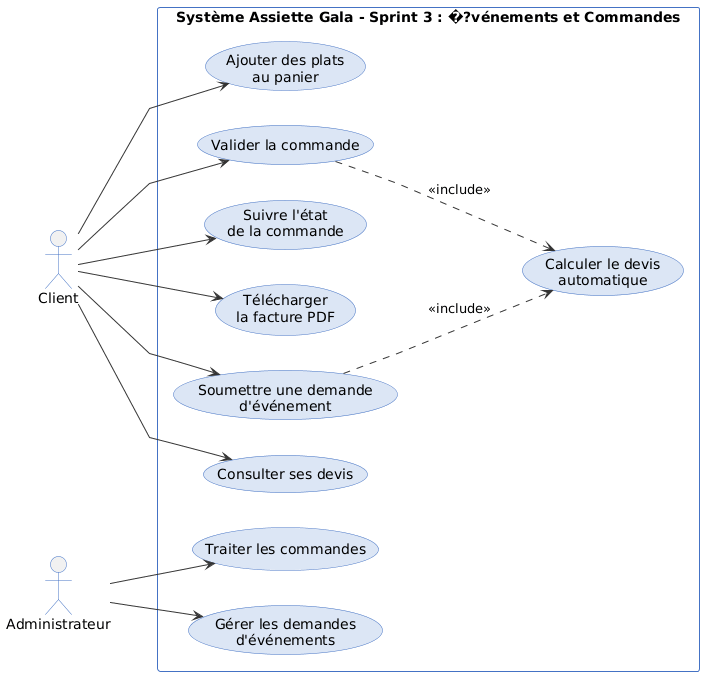
\includegraphics[width=0.85\textwidth]{uc_sprint3.png}
    \caption{Diagramme de cas d'utilisation du sprint 3}
    \label{fig:uc_sprint3}
\end{figure}

\subsection{Description textuelle des cas d'utilisation}

\subsubsection{Cas d'utilisation : Soumettre une demande d'événement}

\begin{table}[H]
    \centering
    \caption{Description textuelle : Soumettre une demande d'événement}
    \label{tab:desc_demande_event}
    \renewcommand{\arraystretch}{1.3}
    \begin{tabular}{|p{4cm}|p{8.5cm}|}
        \hline
        \textbf{Cas d'utilisation} & Soumettre une demande d'événement \\
        \hline
        \textbf{Acteur principal} & Client \\
        \hline
        \textbf{Précondition} & Le client est authentifié \\
        \hline
        \textbf{Postcondition} & La demande est créée avec le statut PENDING \\
        \hline
        \textbf{Scénario principal} &
        \begin{enumerate}
            \item Le futur marié (ou l'organisateur) ouvre le module de planification
            \item Spécification de la nature de la cérémonie (Fiançailles, Séminaire)
            \item Paramétrage du nombre d'invités, de l'adresse de la salle et du jour J
            \item Saisie des exigences particulières (ex: "Aucune viande rouge")
            \item Sélection minutieuse de la composition du buffet
            \item L'algorithme dresse une enveloppe budgétaire brute
            \item Envoi du dossier complet à la direction
            \item Cloche de notification chez l'administrateur
        \end{enumerate} \\
        \hline
        \textbf{Scénario alternatif} &
        \begin{itemize}
            \item[3a.] Réservation dans le passé impossible : le calendrier grise ces jours
            \item[3b.] Surcharge de la capacité maximale du traiteur : jauge bloquante
        \end{itemize} \\
        \hline
    \end{tabular}
\end{table}

\subsection{Description textuelle des cas d'utilisation}

\subsubsection{Cas d'utilisation : Gérer les demandes d'événements}

\begin{table}[H]
    \centering
    \caption{Description textuelle : Gérer les demandes d'événements}
    \label{tab:desc_gerer_events}
    \renewcommand{\arraystretch}{1.3}
    \begin{tabular}{|p{4cm}|p{8.5cm}|}
        \hline
        \textbf{Cas d'utilisation} & Gérer les demandes d'événements \\
        \hline
        \textbf{Acteur principal} & Administrateur \\
        \hline
        \textbf{Précondition} & L'administrateur est authentifié \\
        \hline
        \textbf{Postcondition} & La demande est traitée (confirmée, annulée ou maintenue en attente) \\
        \hline
        \textbf{Scénario principal} &
        \begin{enumerate}
            \item Interception du dossier de réception par le pôle administratif
            \item Ouverture de la fiche détaillée du futur banquet
            \item Audit de la jauge d'invités et des spécificités demandées
            \item Surfacturation éventuelle (frais kilométriques, service à table)
            \item Cachet final de l'entreprise : "Accepté" ou "Désolé, indisponible"
        \end{enumerate} \\
        \hline
    \end{tabular}
\end{table}

\subsection{Partie 2 : Gestion des Commandes et Panier}

\subsection{Conception des commandes}

\subsubsection{Cas d'utilisation : Passer une commande}

\begin{table}[H]
    \centering
    \caption{Description textuelle : Passer une commande}
    \label{tab:desc_passer_commande}
    \renewcommand{\arraystretch}{1.3}
    \begin{tabular}{|p{4cm}|p{8.5cm}|}
        \hline
        \textbf{Cas d'utilisation} & Passer une commande \\
        \hline
        \textbf{Acteur principal} & Client \\
        \hline
        \textbf{Précondition} & Le client est authentifié et son panier contient au moins un plat \\
        \hline
        \textbf{Postcondition} & La commande est créée avec le statut PENDING \\
        \hline
        \textbf{Scénario principal} &
        \begin{enumerate}
            \item L'appétit aiguisé, l'acheteur clique sur l'icône de sa besace (panier)
            \item Présentation d'un bref ticket reprenant les repas et la TVA
            \item Renseignement de l'adresse de livraison (domicile ou travail)
            \item Indication de la volonté d'être livré ou de récupérer sur place
            \item Le bouton de validation déclenche l'envoi vers le backend
            \item PostgreSQL réceptionne et fige le dossier en statut "En attente"
            \item Affichage d'un reçu d'écran avec l'exigence du montant en espèce
        \end{enumerate} \\
        \hline
        \textbf{Précondition} & Le client est authentifié et a des articles dans son panier \\
        \hline
        \textbf{Postcondition} & La commande est enregistrée avec le statut PENDING \\
        \hline
        \textbf{Scénario principal} &
        \begin{enumerate}
            \item Le client valide son panier virtuel
            \item Sélection du mode de livraison (Sur place ou Domicile)
            \item Saisie de l'adresse de livraison le cas échéant
            \item Confirmation du paiement en espèces à la livraison
            \item Enregistrement en base de données et vidage du panier
        \end{enumerate} \\
        \hline
    \end{tabular}
\end{table}

\subsection{Diagrammes de séquence}

\subsubsection{Passage d'une commande}

\begin{figure}[H]
    \centering
    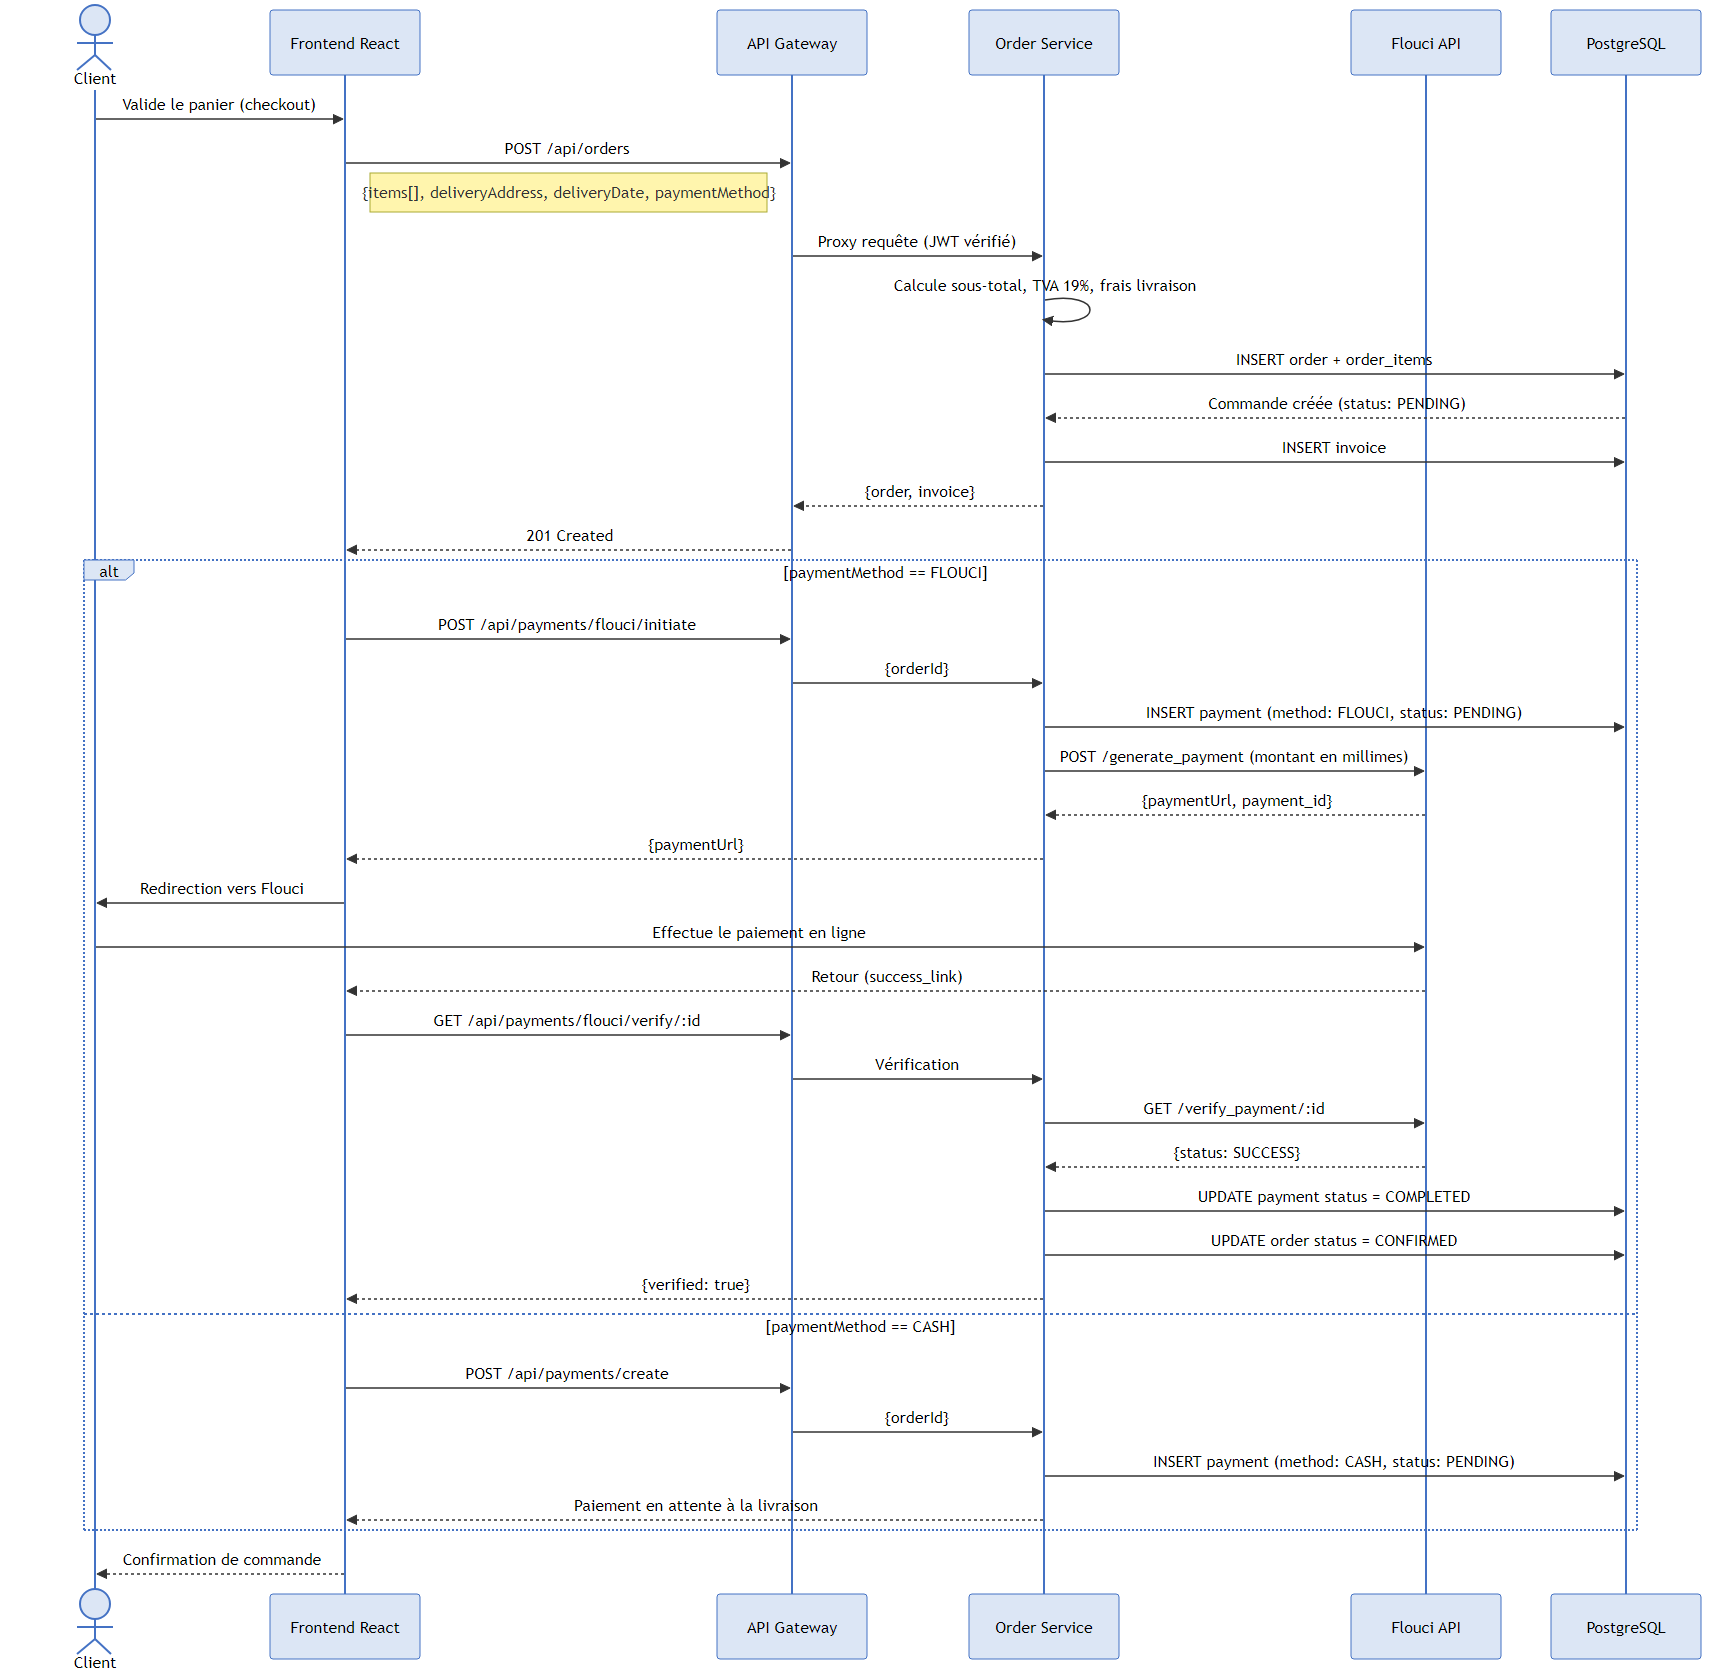
\includegraphics[width=0.9\textwidth]{seq_commande_paiement.png}
    \caption{Diagramme de séquence : Passage d'une commande avec paiement}
    \label{fig:seq_commande}
\end{figure}

\subsubsection{Soumission d'une demande d'événement}

\begin{figure}[H]
    \centering
    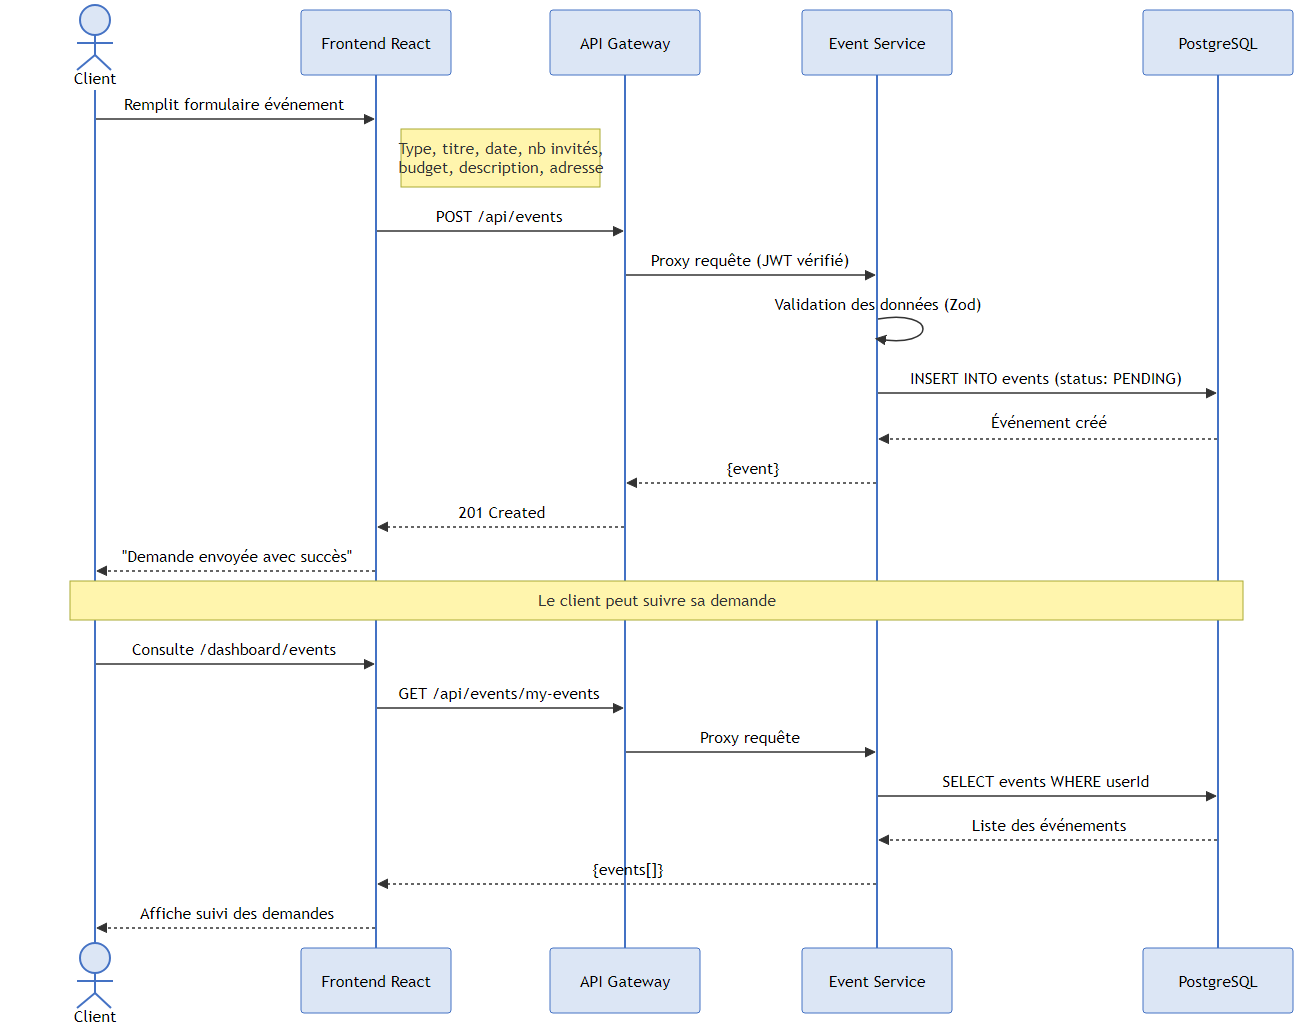
\includegraphics[width=0.9\textwidth]{seq_demande_event.png}
    \caption{Diagramme de séquence : Soumission d'une demande d'événement}
    \label{fig:seq_demande_event}
\end{figure}

\subsubsection{Traitement d'un événement par l'administrateur}

\begin{figure}[H]
    \centering
    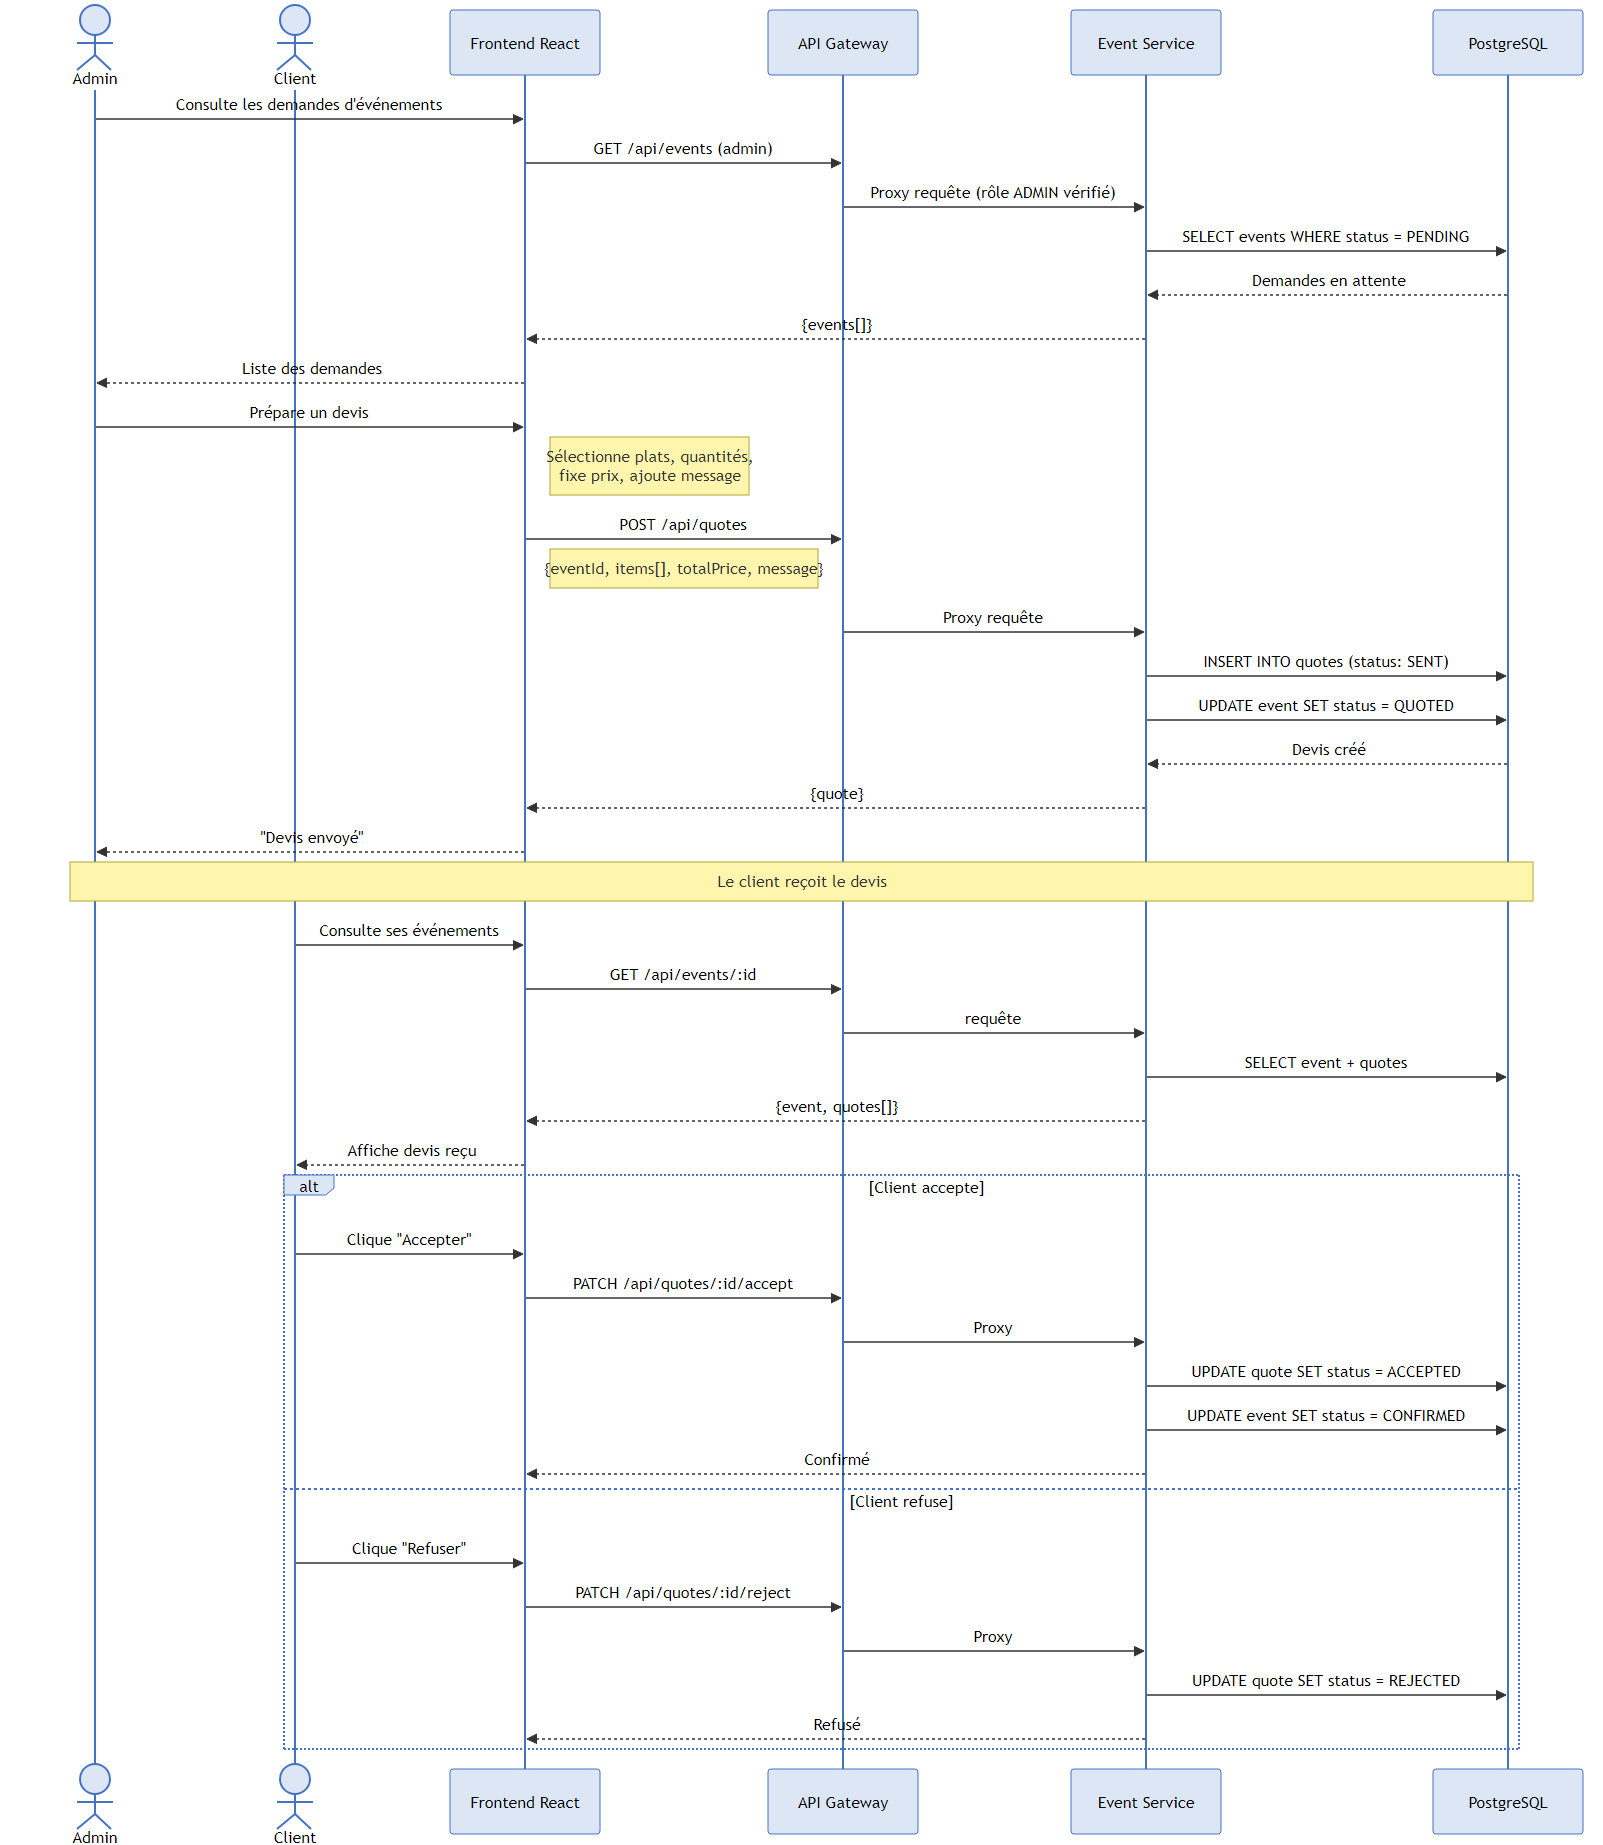
\includegraphics[width=0.9\textwidth]{seq_traitement_event.png}
    \caption{Diagramme de séquence : Traitement d'un événement}
    \label{fig:seq_traitement_event}
\end{figure}

\subsection{Diagramme de classes}

\begin{figure}[H]
    \centering
    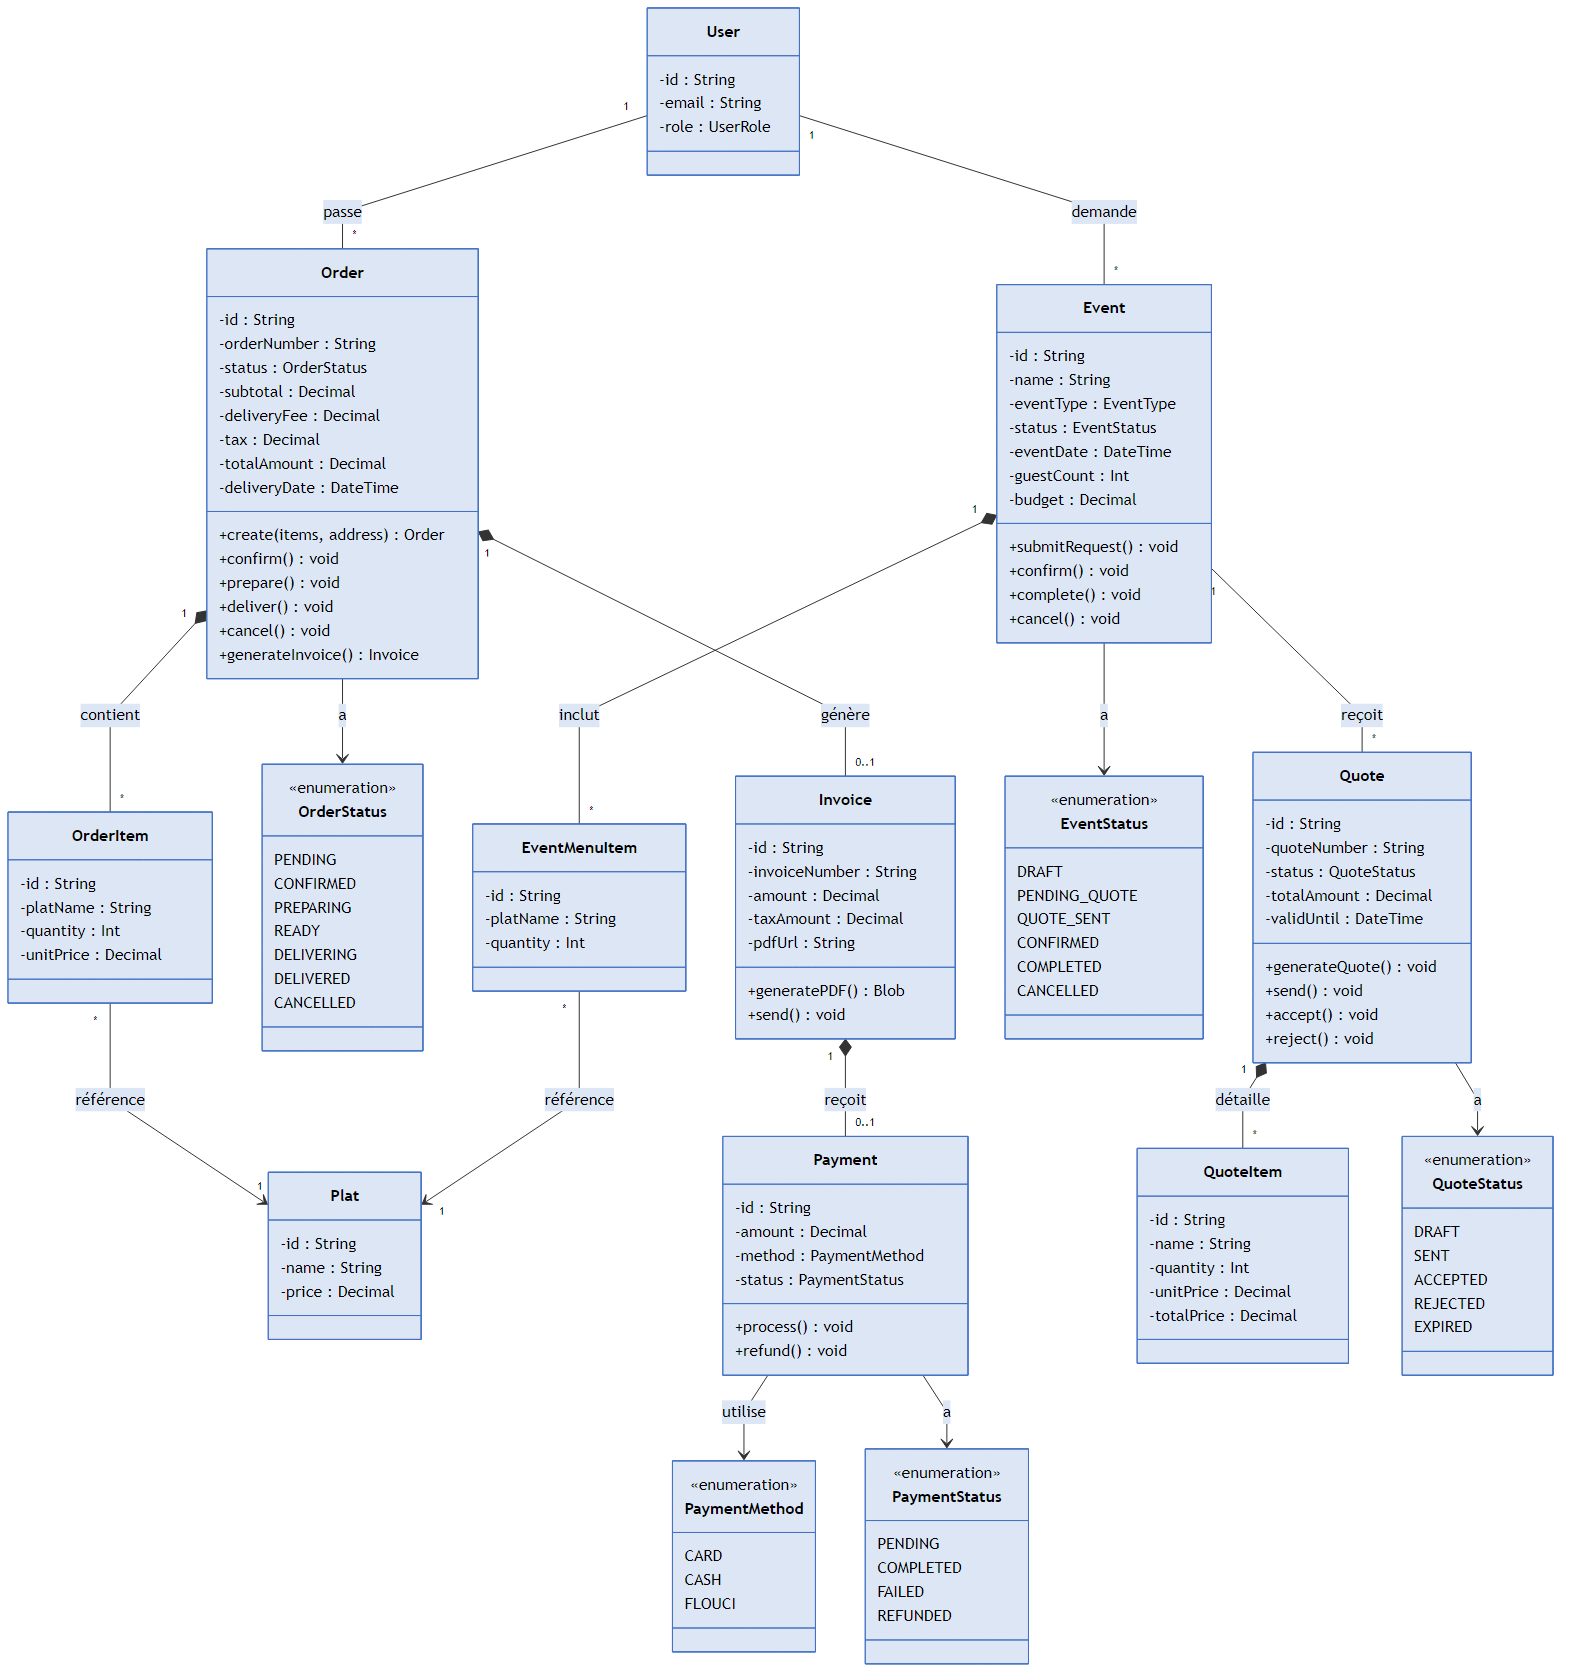
\includegraphics[width=0.95\textwidth]{class_sprint3.png}
    \caption{Diagramme de classes du sprint 3 : Commandes et Événements}
    \label{fig:class_sprint3}
\end{figure}

\subsection{Diagramme d'états-transitions}

\subsubsection{Cycle de vie d'une commande}

\begin{figure}[H]
    \centering
    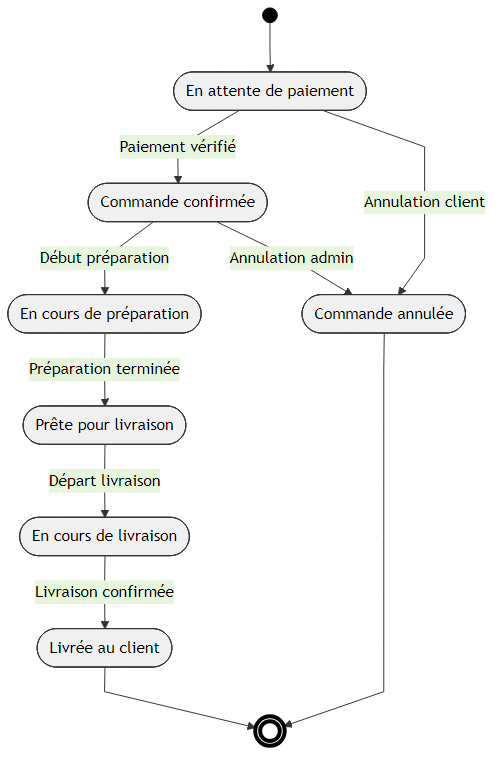
\includegraphics[width=0.85\textwidth]{state_sprint3_order.png}
    \caption{Diagramme d'états-transitions : Commande}
    \label{fig:state_order}
\end{figure}

\subsubsection{Cycle de vie d'un événement}

\begin{figure}[H]
    \centering
    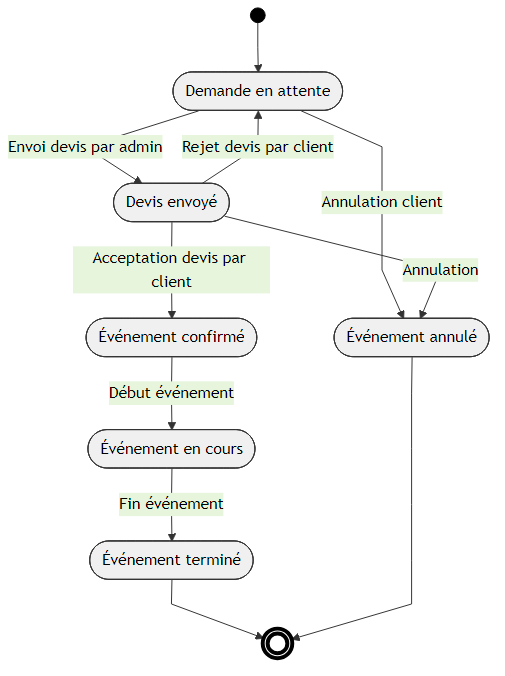
\includegraphics[width=0.85\textwidth]{state_sprint3_event.png}
    \caption{Diagramme d'états-transitions : Événement}
    \label{fig:state_event}
\end{figure}
% --------------------------------------------------
\section{Réalisation}

\subsection{Gestion du paiement en espèces}

Dans le tissu commercial sfaxien, la grande majorité des transactions traiteur s'effectuent en liquide au moment de la réception du plateau. Nous avons donc bâti un circuit qui épouse cette habitude locale plutôt que de la contredire :

\begin{enumerate}
    \item \textbf{Dépôt de la demande :} l'acheteur finalise son panier en ligne ; la commande atterrit dans PostgreSQL avec l'étiquette \texttt{PENDING}.
    \item \textbf{Acquittement par le gérant :} M. Daoud ouvre le panneau d'administration, vérifie la faisabilité (stock, disponibilité de la date) et bascule le dossier en \texttt{PROCESSING}.
    \item \textbf{Règlement physique :} le livreur perçoit la liasse de billets au seuil du client.
    \item \textbf{Clôture comptable :} un clic fait passer le statut à \texttt{COMPLETED}, verrouillant la traçabilité financière.
\end{enumerate}

Ce modèle supprime toute friction liée aux passerelles bancaires et élimine les commissions tierces, tout en conservant un audit trail complet dans la base de données.

\subsection{Limitation de débit sur les commandes}

Pour prévenir les abus (commandes massives automatisées, attaques par déni de service), un \textbf{limiteur de débit} (\texttt{express-rate-limit}) est appliqué sur la route de création de commandes. Ce mécanisme plafonne le nombre de commandes à 5 par minute par utilisateur (identifié par son jeton JWT ou son adresse IP), garantissant un usage raisonnable du service.

\subsection{Jeton de service interne}

Lorsque le service de commandes interroge le service de catalogue pour récupérer les informations d'un plat (prix, nom, disponibilité), il joint un \textbf{jeton de service interne} (\texttt{INTERNAL\_SERVICE\_TOKEN}) dans l'en-tête de la requête. Ce jeton permet au catalogue de vérifier que la requête provient d'un service de confiance, et non d'un acteur externe non autorisé.

\subsection{Configuration dynamique des paramètres de commande}

Plutôt que de coder en dur les frais de livraison, le taux de TVA et le montant minimum de commande dans le frontend, ces paramètres sont exposés via un endpoint \texttt{/api/orders/config}. Le frontend les récupère dynamiquement au chargement de la page de validation, ce qui permet à l'administrateur de modifier ces valeurs sans redéployer l'interface.

\subsection{Génération centralisée des numéros de facture et de commande}

Les fonctions de génération des numéros de facture (format \texttt{INV-YYYYMM-<hex>}) et de commande (format \texttt{ORD-YYMMDD-<hex>}) sont centralisées dans le package partagé \texttt{@traiteurpro/shared}. Cette déduplication garantit un format unique et cohérent entre le service de commandes et le service de paiement, éliminant le risque de divergence ou de doublon.

\subsection{Génération de factures PDF}

Chaque transaction validée peut donner lieu à une pièce comptable imprimable, forgée à la volée par le module \texttt{PDFKit}. Le document embarque :

\begin{itemize}
    \item Le cartouche Assiette Gala (logo, adresse Route Mahdia km 1, téléphone)
    \item Les coordonnées de l'acheteur
    \item La référence UUID et la date de captation
    \item La ventilation détaillée (dénomination, quantité, prix HT, sous-total)
    \item Le total TTC incluant la TVA à 19\,\%
    \item La mention de l'état du règlement
\end{itemize}

Le fichier binaire est assemblé en mémoire vive puis projeté vers le navigateur avec l'entête \texttt{Content-Type: application/pdf}, déclenchant le téléchargement immédiat.

\subsection{Interfaces réalisées}

\subsubsection{Panier d'achat}

% FIGURE UI REMOVED : Add screenshot later

Le panier récapitule la sélection du gourmand : chaque ligne dévoile la vignette du mets, son tarif unitaire et un compteur incrémentable. Le bas de page totalise la facture prévisionnelle, invitant l'acheteur à modifier ou élaguer avant de poursuivre.

\subsubsection{Page de validation de commande}

% FIGURE UI REMOVED : Add screenshot later

Cet écran rassemble en un coup d'\oe{}il le résumé du panier, le choix de l'adresse de livraison et le mode de réception (livraison à domicile ou retrait Route Mahdia). Le total TTC en dinars tunisiens, calculé avec une TVA de 19\,\%, est mis en évidence.

\subsubsection{Historique des commandes}

% FIGURE UI REMOVED : Add screenshot later

Le journal personnel du client empile ses achats passés du plus récent au plus ancien : date, montant déboursé et pastille colorée (jaune = en attente, vert = livré, rouge = annulé). Un lien ouvre la fiche détaillée de chaque dossier.

\subsubsection{Gestion des commandes (Administrateur)}

% FIGURE UI REMOVED : Add screenshot later

Le poste de contrôle de M. Daoud dresse un inventaire filtré par état. D'un clic, il fait progresser une commande de \texttt{PROCESSING} vers \texttt{COMPLETED}, et peut ouvrir le détail complet (coordonnées, plats, montant) de chaque opération.

% --------------------------------------------------
\section{Tests fonctionnels}

\begin{table}[H]
    \centering
    \caption{Tests fonctionnels : Sprint 4}
    \label{tab:tests_sprint4}
    \renewcommand{\arraystretch}{1.3}
    \begin{tabular}{|c|p{3cm}|p{3.5cm}|p{2.5cm}|}
        \hline
        \textbf{N°} & \textbf{Cas de test} & \textbf{Comportement attendu} & \textbf{Résultat} \\
        \hline
        1 & Ajout d'un plat au panier & Plat ajouté, quantité et total mis à jour & Réussi \\
        \hline
        2 & Modification de la quantité dans le panier & Sous-total et total recalculés & Réussi \\
        \hline
        3 & Suppression d'un article du panier & Article retiré, total recalculé & Réussi \\
        \hline
        4 & Validation de la commande & Commande créée en base, statut PENDING & Réussi \\
        \hline
        5 & Paiement en espèces confirmé & Statut mis à jour à COMPLETED par l'administrateur & Réussi \\
        \hline
        6 & Annulation de commande & Statut mis à jour à CANCELLED, message affiché & Réussi \\
        \hline
        7 & Téléchargement de facture PDF & PDF généré contenant tous les détails & Réussi \\
        \hline
        8 & Consultation de l'historique & Liste des commandes avec statuts corrects & Réussi \\
        \hline
        9 & Mise à jour du statut par l'administrateur & Statut modifié en base et sur l'interface & Réussi \\
        \hline
        10 & Commande sans authentification & Redirection vers la page de connexion & Réussi \\
        \hline
    \end{tabular}
\end{table}

% --------------------------------------------------
\section*{Conclusion}
\addcontentsline{toc}{section}{Conclusion}

\begin{samepage}
À l'issue de cet acte de programmation, Assiette Gala jouit d'une caisse enregistreuse immatérielle connectée directement à sa cuisine. Le traitement du panier, calqué sur le comportement tunisien du "paiement à l'arrivée", garantit une conversion commerciale maximale car débarrassé de la friction des cartes bleues. Fort de cette ossature financière, le Sprint 5 peut s'atteler au tableau de bord analytique.
\end{samepage}



% Chapitre 6 (Sprint 4) : Back-Office et Analytics (teal)
\clearpage
\renewcommand{\currentchapcolor}{chap-dashboard}
% ============================================================
% CHAPITRE 6 (Sprint 4)
% ============================================================
\chapter{Sprint 4 : Back-Office et Analytics}

\section{Introduction}

Le Sprint 4 marque la transition vers l'administration globale de la plateforme Assiette Gala. Si les sprints précédents se sont focalisés sur la construction de l'expérience d'achat (vitrine, commandes, événements), ce sprint vise à fournir à la direction les outils de pilotage stratégique de l'entreprise. 

Ce cycle consolide l'ensemble du "Back-Office" : le tableau de bord analytique, le contrôle des flux financiers (dépenses, encaissements), le pilotage des stocks et des fournisseurs, ainsi que la génération des documents comptables légaux (factures, bons de commande). Le but est de remplacer tous les registres papier par un système d'information centralisé.

% --------------------------------------------------
\section{Backlog du sprint}

Le Tableau~\ref{tab:backlog_sprint4_admin} recense les user stories priorisées pour ce sprint.

\begin{table}[H]
    \centering
    \caption{Backlog du sprint 4 : Back-Office et Analytics}
    \label{tab:backlog_sprint4_admin}
    \renewcommand{\arraystretch}{1.3}
    \begin{tabular}{|c|p{8.5cm}|c|}
        \hline
        \textbf{ID} & \textbf{User Story} & \textbf{Durée (jours)} \\
        \hline
        US-18 & En tant qu'administrateur, je souhaite visualiser des KPI et graphiques d'évolution afin de piloter l'activité. & 4 \\
        \hline
        US-19 & En tant qu'administrateur, je souhaite analyser la répartition des commandes par statut et les tendances. & 2 \\
        \hline
        US-20 & En tant qu'administrateur, je souhaite suivre les flux financiers (caisse, dépenses) pour garantir la rentabilité. & 3 \\
        \hline
        US-21 & En tant qu'administrateur, je souhaite générer des documents comptables au format PDF. & 3 \\
        \hline
    \end{tabular}
\end{table}

% --------------------------------------------------
\section{Partie A : Tableau de Bord et Analytics}

\subsection{Architecture du système de reporting}

Le module d'analytics repose sur une architecture en trois couches :
\begin{enumerate}
    \item \textbf{Base de données (Prisma) :} Utilisation de la fonction \texttt{groupBy} et des agrégations SQL pour consolider les données côté serveur sans surcharger la mémoire Node.js.
    \item \textbf{API Gateway :} Un contrôleur dédié aux statistiques orchestre les appels concurrents via \texttt{Promise.all()} pour minimiser le temps de réponse.
    \item \textbf{Frontend (Recharts) :} Les données brutes sont transformées et injectées dans des composants graphiques interactifs (SVG) fluides.
\end{enumerate}

\subsection{Indicateurs de Performance (KPI)}

Le tableau de bord supérieur offre une vue synthétique des métriques vitales :
\begin{itemize}
    \item Chiffre d'affaires total (avec comparaison par rapport au mois précédent).
    \item Nombre de commandes et taux de validation.
    \item Panier moyen.
    \item Volume d'événements en attente de traitement.
\end{itemize}

\subsection{Visualisations Graphiques}

L'interface analytique intègre plusieurs graphiques interactifs :
\begin{itemize}
    \item \textbf{Courbe d'évolution des revenus :} Permet d'identifier la saisonnalité de l'activité.
    \item \textbf{Diagramme en beignet (Donut Chart) :} Répartition des commandes par statut (En attente, En préparation, Livré).
    \item \textbf{Graphique en barres :} Palmarès des plats les plus vendus (Top 5).
\end{itemize}

% --------------------------------------------------
\section{Partie B : Suivi des Flux Financiers}

Le module finance assure le suivi complet des mouvements monétaires, consolidant les ventes issues du module de commandes et les charges de fonctionnement :

\begin{itemize}
    \item \textbf{Encaissements} : Visualisation des entrées d'argent par mode de paiement, automatiquement alimentée par le changement de statut des commandes (passage en "Complété").
    \item \textbf{Dépenses (Charges) :} Interface permettant l'enregistrement des sorties financières (factures fournisseurs, achats de matières premières, charges fixes) avec catégorisation.
    \item \textbf{Balance} : Calcul du flux net de trésorerie sur la période sélectionnée.
\end{itemize}

% --------------------------------------------------
\section{Partie C : Gestion Documentaire (PDF)}

La génération de documents légaux constitue la dernière brique de l'ERP métier. Le module documentaire permet la création à la volée de :

\begin{itemize}
    \item \textbf{Factures (Invoices) :} Génération dynamique via le package \texttt{pdfkit}. Les factures intègrent le logo d'Assiette Gala, les mentions légales tunisiennes, la numérotation séquentielle inviolable (format \texttt{INV-YYYYMM-<hex>}), le détail des lignes de commande et le calcul de la TVA à 19\%.
    \item \textbf{Bons de commande fournisseurs :} Documents d'achat liant les besoins en stock aux fournisseurs enregistrés.
\end{itemize}

% --------------------------------------------------
\section{Conception}

\subsection{Diagramme de cas d'utilisation}

\begin{figure}[H]
    \centering
    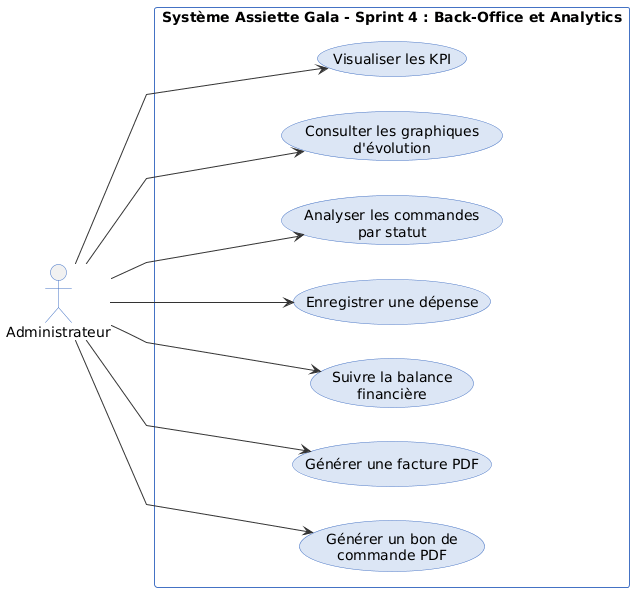
\includegraphics[width=0.85\textwidth]{uc_sprint4.png}
    \caption{Diagramme de cas d'utilisation : Back-Office et Analytics}
    \label{fig:uc_sprint4}
\end{figure}

\subsection{Description textuelle des cas d'utilisation}

\subsubsection{Cas d'utilisation : Visualiser les KPI}

\begin{table}[H]
    \centering
    \caption{Description textuelle : Visualiser les KPI}
    \label{tab:desc_kpi}
    \renewcommand{\arraystretch}{1.3}
    \begin{tabular}{|p{4cm}|p{8.5cm}|}
        \hline
        \textbf{Cas d'utilisation} & Visualiser les KPI et graphiques \\
        \hline
        \textbf{Acteur principal} & Administrateur \\
        \hline
        \textbf{Précondition} & Authentifié avec le rôle \texttt{ADMIN} \\
        \hline
        \textbf{Postcondition} & Les indicateurs sont affichés à jour \\
        \hline
        \textbf{Scénario principal} &
        \begin{enumerate}
            \item L'administrateur accède à la page d'accueil du Dashboard
            \item Le système interroge l'API Gateway (\texttt{/api/stats/overview})
            \item L'API consolide les données via Prisma (\texttt{groupBy})
            \item Affichage des cartes animées (CA, Commandes)
            \item Rendu des graphiques Recharts (Courbe de revenus, Donut des statuts)
        \end{enumerate} \\
        \hline
    \end{tabular}
\end{table}

\subsubsection{Cas d'utilisation : Suivre les flux financiers}

\begin{table}[H]
    \centering
    \caption{Description textuelle : Flux financiers}
    \label{tab:desc_finance}
    \renewcommand{\arraystretch}{1.3}
    \begin{tabular}{|p{4cm}|p{8.5cm}|}
        \hline
        \textbf{Cas d'utilisation} & Enregistrer une dépense et suivre la caisse \\
        \hline
        \textbf{Acteur principal} & Administrateur \\
        \hline
        \textbf{Précondition} & Authentifié avec le rôle \texttt{ADMIN} \\
        \hline
        \textbf{Postcondition} & La dépense est enregistrée, la balance financière est mise à jour \\
        \hline
        \textbf{Scénario principal} &
        \begin{enumerate}
            \item Navigation vers le module "Finance"
            \item Saisie d'une facture fournisseur (ex: 500 TND pour viandes)
            \item Validation du formulaire
            \item Le système déduit le montant des encaissements globaux
            \item Inscription de la transaction dans le journal d'audit
        \end{enumerate} \\
        \hline
    \end{tabular}
\end{table}

\subsubsection{Cas d'utilisation : Générer un document PDF}

\begin{table}[H]
    \centering
    \caption{Description textuelle : Documents comptables}
    \label{tab:desc_pdf}
    \renewcommand{\arraystretch}{1.3}
    \begin{tabular}{|p{4cm}|p{8.5cm}|}
        \hline
        \textbf{Cas d'utilisation} & Générer une facture au format PDF \\
        \hline
        \textbf{Acteur principal} & Administrateur / Client \\
        \hline
        \textbf{Précondition} & Commande clôturée (\texttt{COMPLETED}) \\
        \hline
        \textbf{Postcondition} & Fichier PDF téléchargé \\
        \hline
        \textbf{Scénario principal} &
        \begin{enumerate}
            \item Clic sur le bouton d'export PDF de la commande
            \item Le module \texttt{pdfkit} dessine l'en-tête (Logo Assiette Gala, Matricule)
            \item Itération sur les lignes de la commande pour tracer le tableau
            \item Calcul de la TVA et du TTC
            \item Envoi du flux binaire en téléchargement
        \end{enumerate} \\
        \hline
    \end{tabular}
\end{table}

\subsection{Diagrammes de séquence}

\subsubsection{Chargement du tableau de bord}

\begin{figure}[H]
    \centering
    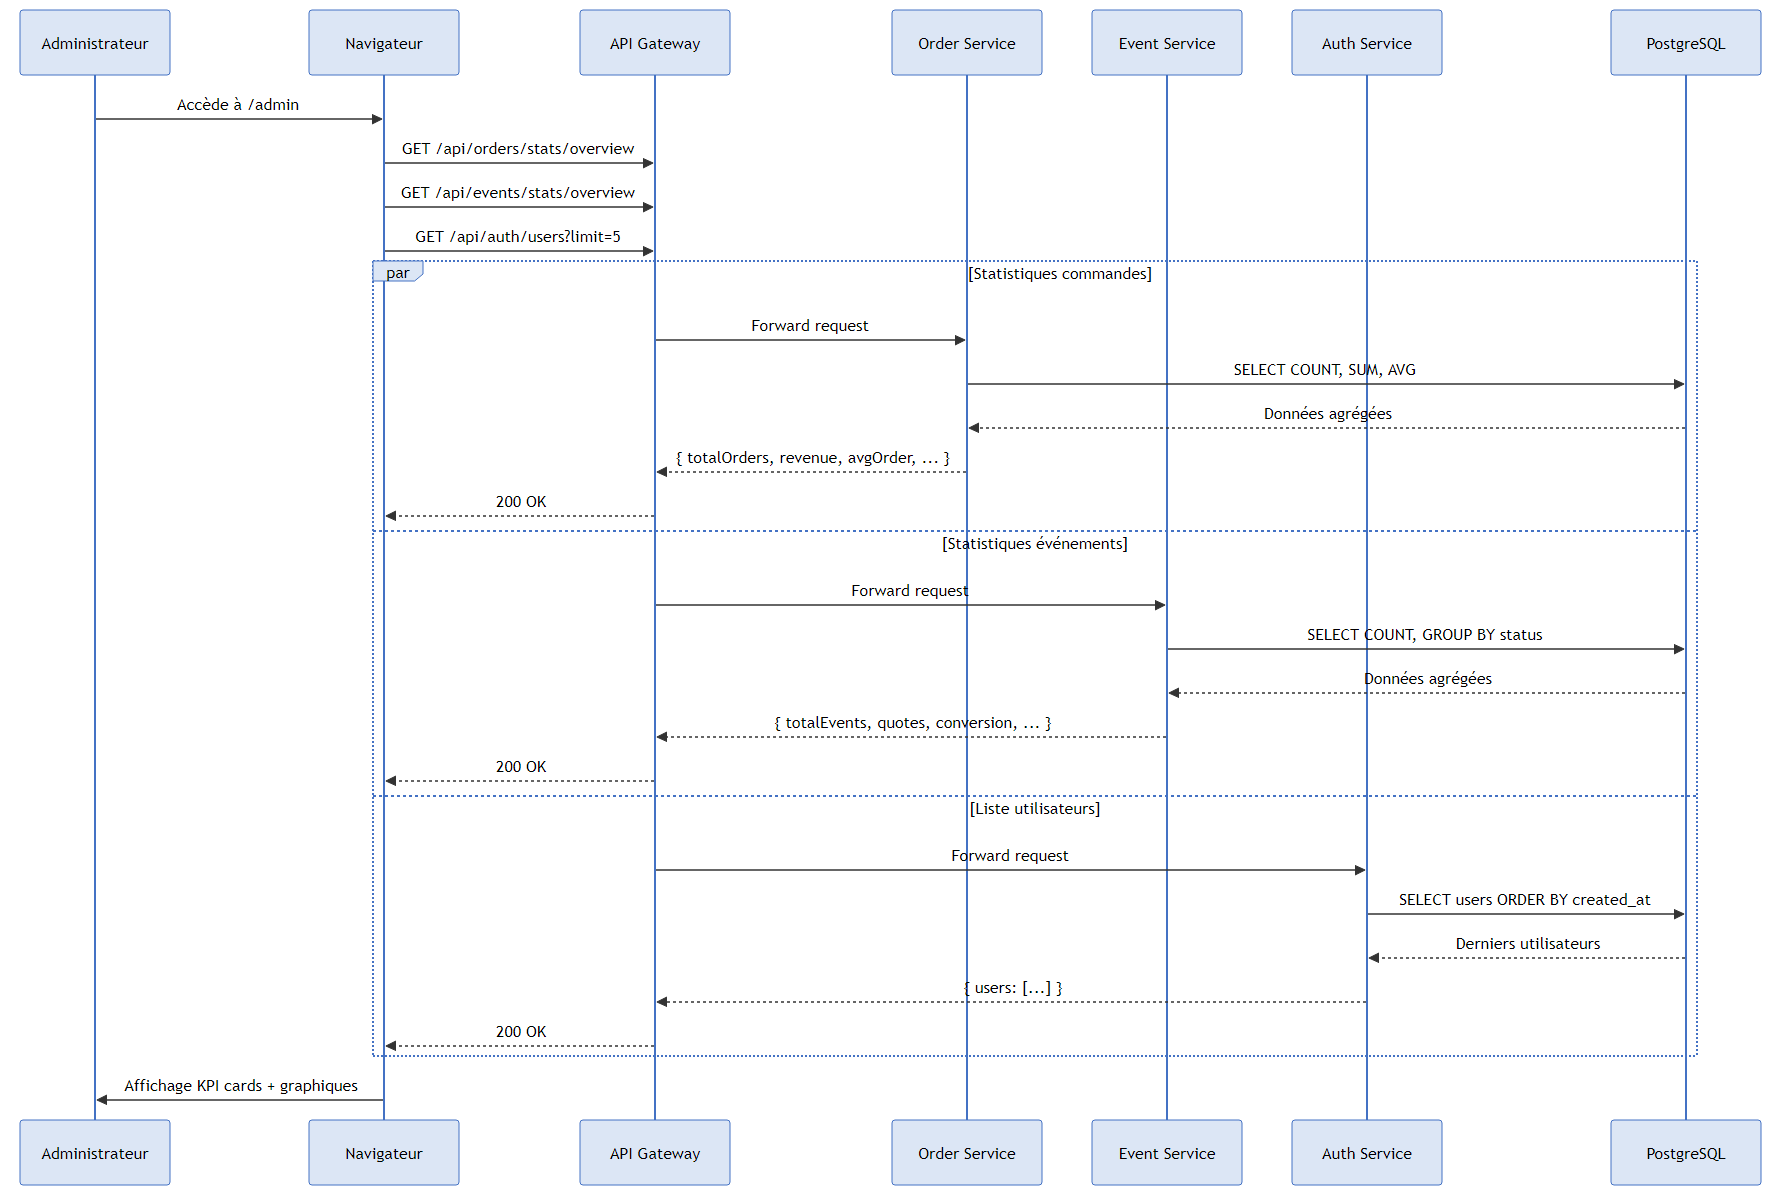
\includegraphics[width=0.9\textwidth]{seq_dashboard_load.png}
    \caption{Diagramme de séquence : Chargement du Dashboard}
    \label{fig:seq_dashboard}
\end{figure}

\subsubsection{Génération d'une facture PDF}

\begin{figure}[H]
    \centering
    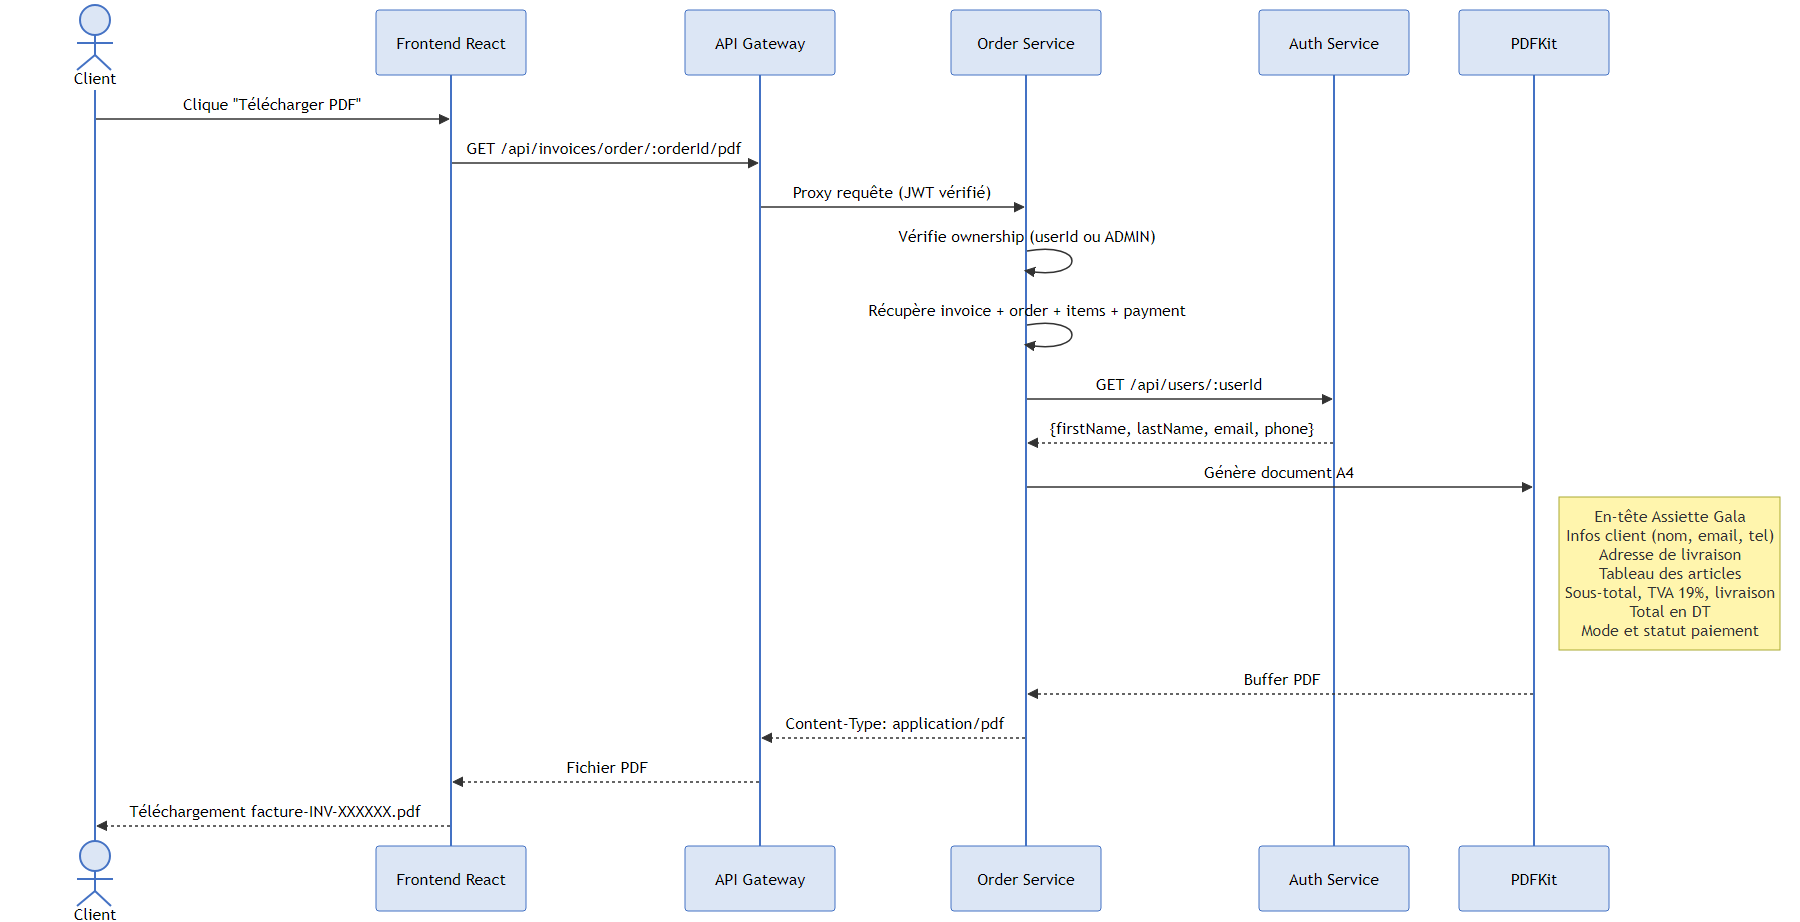
\includegraphics[width=0.9\textwidth]{seq_facture.png}
    \caption{Diagramme de séquence : Génération de facture PDF}
    \label{fig:seq_facture}
\end{figure}

\subsubsection{Filtrage des statistiques par période}

\begin{figure}[H]
    \centering
    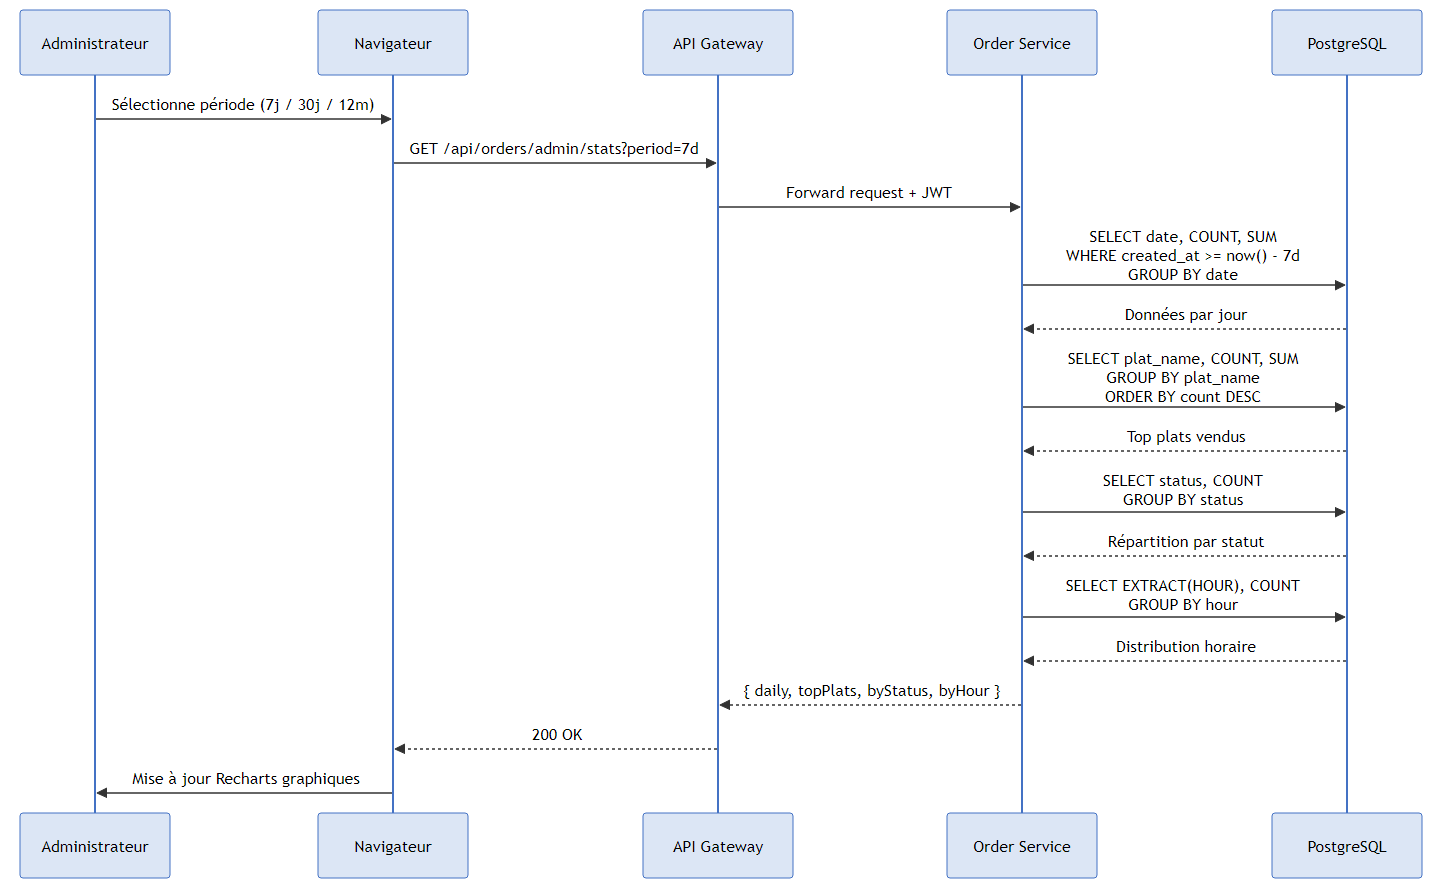
\includegraphics[width=0.9\textwidth]{seq_stats_filter.png}
    \caption{Diagramme de séquence : Filtrage des statistiques par période}
    \label{fig:seq_stats_filter}
\end{figure}

\subsection{Diagramme de classes}

\begin{figure}[H]
    \centering
    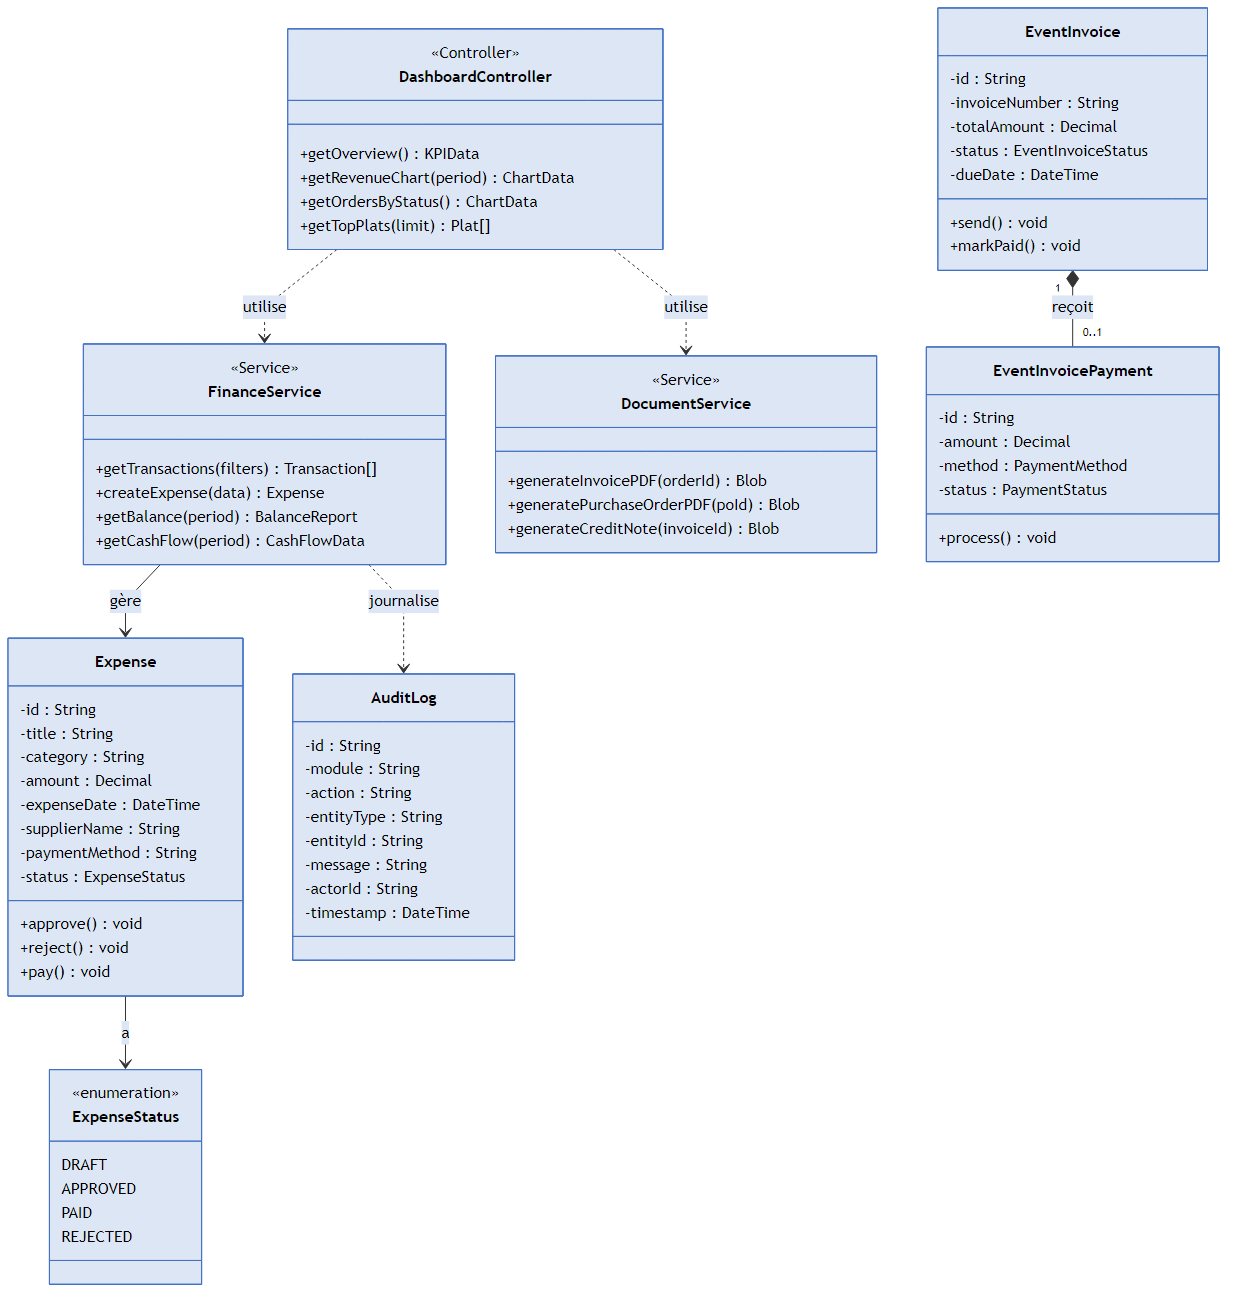
\includegraphics[width=0.95\textwidth]{class_sprint4.png}
    \caption{Diagramme de classes du sprint 4 : Back-Office et Analytics}
    \label{fig:class_sprint4}
\end{figure}
% --------------------------------------------------
\section{Réalisation technique}

\subsection{Points d'entrée de l'API}

\begin{table}[H]
    \centering
    \caption{Endpoints REST du Back-Office}
    \label{tab:endpoints_admin}
    \renewcommand{\arraystretch}{1.2}
    \begin{tabular}{|l|p{4.5cm}|p{5.5cm}|}
        \hline
        \textbf{Méthode} & \textbf{Route} & \textbf{Description} \\
        \hline
        GET & /api/stats/overview & Récupération des KPI globaux \\
        \hline
        GET & /api/stats/revenue-chart & Données pour la courbe des revenus \\
        \hline
        GET & /api/finance/transactions & Liste des flux (entrées/sorties) \\
        \hline
        POST & /api/finance/expense & Enregistrement d'une dépense \\
        \hline
        GET & /api/documents/invoice/:id & Génération de facture PDF \\
        \hline
    \end{tabular}
\end{table}

\subsection{Tests fonctionnels}

\begin{table}[H]
    \centering
    \caption{Tests fonctionnels : Sprint 4}
    \label{tab:tests_sprint4}
    \renewcommand{\arraystretch}{1.3}
    \begin{tabular}{|c|p{4cm}|p{4cm}|p{2cm}|}
        \hline
        \textbf{N°} & \textbf{Cas de test} & \textbf{Comportement attendu} & \textbf{Résultat} \\
        \hline
        1 & Accès aux KPI sans token admin & Refus (401 ou 403) & Réussi \\
        \hline
        2 & Calcul du chiffre d'affaires & Somme exacte des commandes livrées & Réussi \\
        \hline
        3 & Enregistrement d'une dépense & Dépense créée et déduite de la balance & Réussi \\
        \hline
        4 & Génération facture PDF & PDF généré avec TVA à 19\% et lignes correctes & Réussi \\
        \hline
    \end{tabular}
\end{table}

% --------------------------------------------------
\section*{Conclusion}
\addcontentsline{toc}{section}{Conclusion}

\begin{samepage}
Ce Sprint 4 transforme la plateforme d'une simple interface de prise de commande en un véritable outil de pilotage (\textbf{ERP allégé}). La direction d'Assiette Gala dispose désormais d'une visibilité totale sur ses indicateurs de croissance, sa trésorerie et l'édition de ses documents comptables.

L'administration étant désormais entièrement digitalisée et outillée, le système est prêt à accueillir le cinquième et dernier sprint : l'intégration de la couche algorithmique d'Intelligence Artificielle.
\end{samepage}



% Chapitre 7 (Sprint 5) : Intelligence Artificielle (doré)
\clearpage
\renewcommand{\currentchapcolor}{chap-ia}
% ============================================================
% CHAPITRE 7 (Sprint 5)
% ============================================================
\chapter{Sprint 5 : Intelligence Artificielle}

\section{Introduction}

Ce cinquième et dernier sprint constitue l'aboutissement technologique de ce projet de Master. Alors que les sprints précédents ont permis de consolider l'architecture transactionnelle (le \textit{CRUD} classique) d'Assiette Gala, cette phase dote le système d'une véritable \textbf{intelligence décisionnelle et conversationnelle}. L'objectif n'est plus seulement d'enregistrer des données, mais de les analyser, de prédire des comportements et d'optimiser les ressources de l'entreprise.

Ce sprint déploie cinq briques majeures d'Intelligence Artificielle : l'assistant conversationnel RAG (Traitement du Langage Naturel), le moteur de recommandation hybride, l'algorithme prédictif des besoins en stock (\textit{Forecasting}), le planificateur intelligent de tâches en cuisine (\textit{Kitchen Optimizer}) et l'extracteur de données de factures par vision artificielle (OCR).

% --------------------------------------------------
\section{Backlog du sprint}

Le Tableau~\ref{tab:backlog_sprint5_ia} synthétise les user stories de ce sprint, dont les durées reflètent la complexité de l'ingénierie algorithmique.

\begin{table}[H]
    \centering
    \caption{Backlog du sprint 5 : Intelligence Artificielle}
    \label{tab:backlog_sprint5_ia}
    \renewcommand{\arraystretch}{1.3}
    \begin{tabular}{|c|p{8.5cm}|c|}
        \hline
        \textbf{ID} & \textbf{User Story} & \textbf{Durée (jours)} \\
        \hline
        US-22 & En tant que visiteur, je souhaite interagir avec un chatbot RAG (NLP) pour des réponses expertes sur le menu. & 5 \\
        \hline
        US-23 & En tant que client, je souhaite recevoir des recommandations de plats basées sur mes goûts. & 4 \\
        \hline
        US-24 & En tant qu'administrateur, je souhaite que le système prévoie les besoins en stocks (Forecasting). & 6 \\
        \hline
        US-25 & En tant que chef cuisinier, je souhaite un ordonnancement intelligent des tâches (Kitchen Optimizer). & 6 \\
        \hline
        US-26 & En tant qu'administrateur, je souhaite scanner des factures pour extraire les données via OCR IA. & 4 \\
        \hline
    \end{tabular}
\end{table}

% ==============================================================
\section{Moteur Conversationnel : Architecture RAG}
% ==============================================================

\subsection{Principes du RAG (Retrieval-Augmented Generation)}

Le chatbot ne s'appuie pas uniquement sur les connaissances pré-entraînées du modèle linguistique, ce qui risquerait de produire des hallucinations. Il utilise une architecture RAG qui intercepte la question, recherche des documents pertinents dans la base de données métier (le catalogue et les tarifs actuels d'Assiette Gala), et force le modèle \textbf{Google Gemini 2.5 Flash} à formuler sa réponse à partir de ce contexte précis.

\subsection{Pipeline d'indexation et de recherche}

\begin{figure}[H]
    \centering
    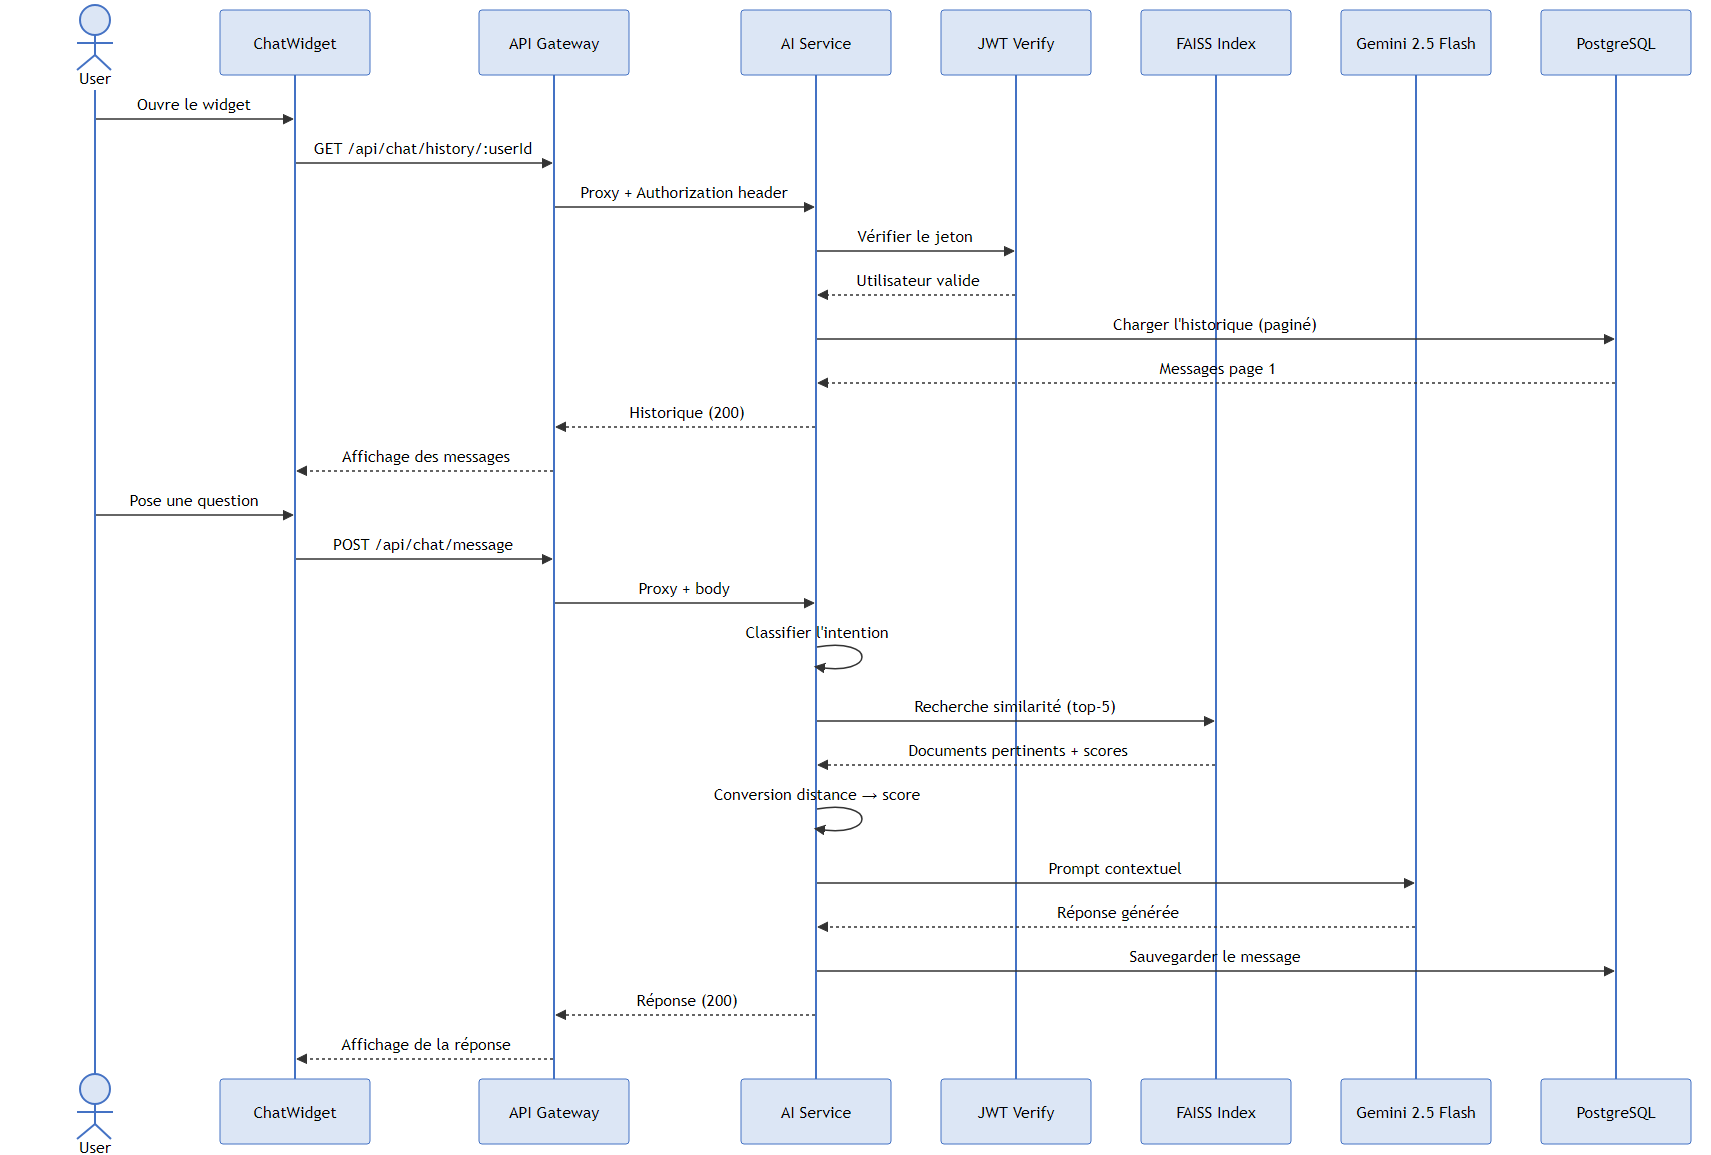
\includegraphics[width=0.95\textwidth]{seq_chatbot.png}
    \caption{Architecture RAG : Indexation vectorielle et Génération}
    \label{fig:rag_pipeline}
\end{figure}

Le pipeline s'articule autour de \textbf{LangChain} et de \textbf{FAISS} (Facebook AI Similarity Search) :
\begin{enumerate}
    \item \textbf{Vectorisation (Embedding) :} Chaque fiche plat est convertie en vecteur dense (384 dimensions) via le modèle \textit{all-MiniLM-L6-v2}.
    \item \textbf{Stockage :} Les vecteurs sont persistés dans une base vectorielle FAISS locale, optimisée pour le calcul de distance L2.
    \item \textbf{Filtrage Sémantique :} Un routeur d'intention classe la requête entrante (\texttt{menu}, \texttt{allergen}, \texttt{event}) pour réduire l'espace de recherche vectorielle.
    \item \textbf{Top-K Retrieval :} FAISS extrait les 5 documents les plus sémantiquement proches de la requête.
    \item \textbf{Prompt Augmenté :} Le contexte extrait est injecté dynamiquement dans un prompt strict avant soumission à Gemini.
\end{enumerate}

\subsection{Rafraîchissement de la base de connaissances}

Le diagramme de séquence suivant (figure~\ref{fig:seq_refresh_knowledge}) illustre le processus d'indexation de la base de connaissances, déclenché par l'administrateur pour synchroniser le catalogue avec l'index vectoriel FAISS.

\begin{figure}[H]
    \centering
    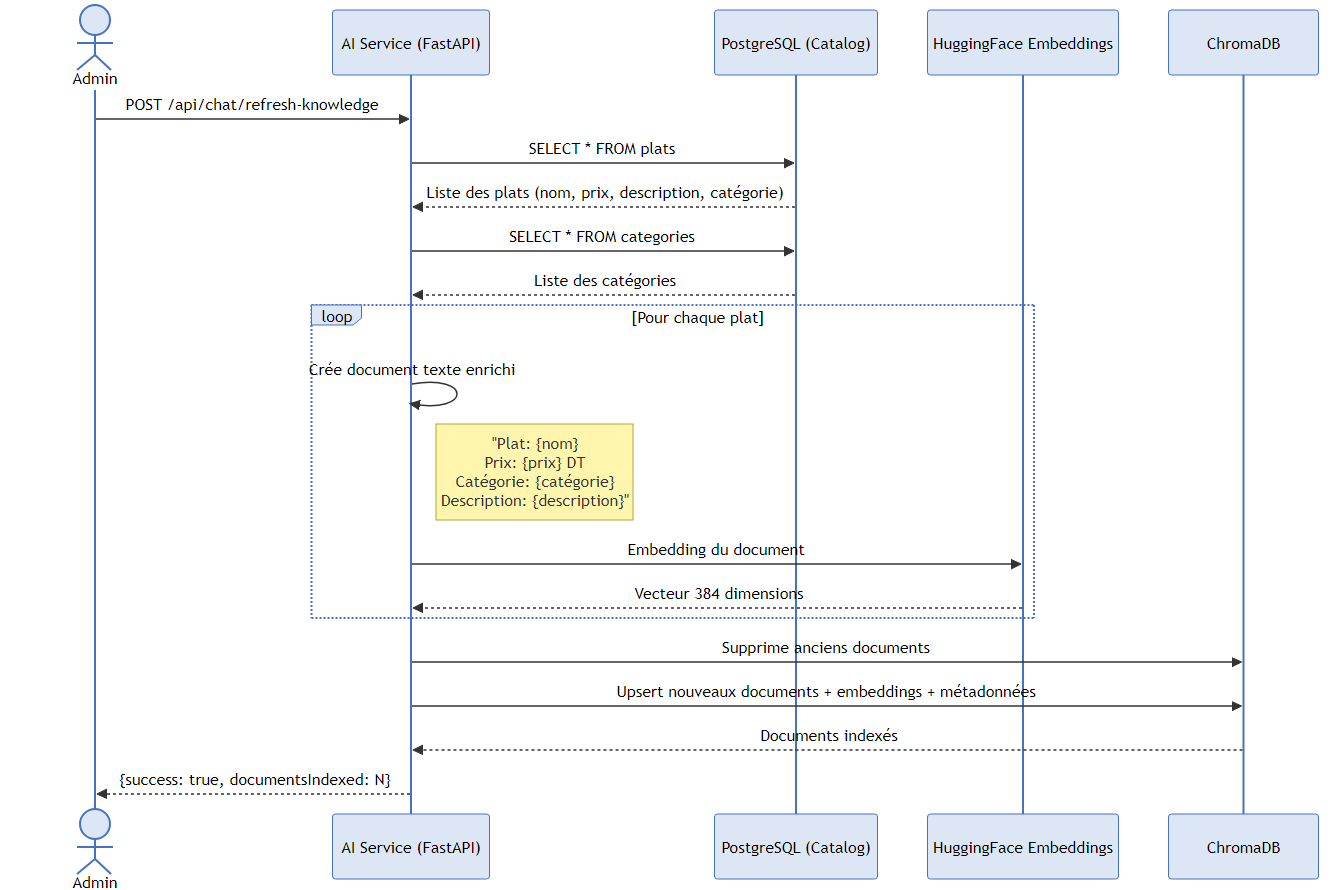
\includegraphics[width=0.9\textwidth]{seq_refresh_knowledge.png}
    \caption{Diagramme de séquence : Rafraîchissement de la base de connaissances}
    \label{fig:seq_refresh_knowledge}
\end{figure}

% ==============================================================
\section{Forecasting Engine : Prévision des Stocks}
% ==============================================================

L'un des défis majeurs d'un traiteur est d'éviter le gaspillage alimentaire tout en prévenant les ruptures de stock. Le \textbf{Forecasting Engine} est un modèle d'analyse prédictive.

\subsection{Algorithme de lissage exponentiel}

Le moteur analyse les séries temporelles des commandes passées (historique de 6 mois). Plutôt que d'utiliser une moyenne mobile simple, il applique un \textbf{lissage exponentiel} qui accorde plus de poids aux tendances récentes et intègre des coefficients de saisonnalité (pics d'événements le week-end).

$$
F_{t+1} = \alpha \cdot D_t + (1 : \alpha) \cdot F_t
$$

Où $F_{t+1}$ est la prévision, $D_t$ la demande réelle, et $\alpha$ le facteur de lissage dynamique. L'algorithme décompose les plats commandés en leurs \textbf{ingrédients bruts} (via une nomenclature), générant ainsi un rapport prédictif des kilos de viande, légumes et épices nécessaires pour les 7 prochains jours.

% ==============================================================
\section{Kitchen Optimizer : Ordonnancement Intelligent}
% ==============================================================

Le \textbf{Kitchen Optimizer} s'attaque au problème complexe de la planification des tâches en cuisine, assimilable au problème d'ordonnancement d'atelier (Job-Shop Scheduling Problem : JSSP).

\subsection{Heuristique d'ordonnancement}

L'algorithme reçoit en entrée un lot de commandes à livrer à une heure précise. Il découpe chaque commande en sous-tâches (préparation, cuisson, dressage) ayant des durées et des dépendances strictes.
En utilisant la \textbf{méthode du chemin critique (CPM)} et une heuristique gloutonne, le système répartit les tâches entre les postes de travail (four, plan de travail, frigo) pour minimiser le temps d'inactivité global (le \textit{makespan}) et garantir que les plats chauds sortent juste avant l'expédition.

% ==============================================================
\section{AI Receipt Scanner : Vision par Ordinateur}
% ==============================================================

Pour automatiser la saisie des charges, le portail intègre un module d'\textbf{Extraction d'Information (OCR structuré)}.

L'administrateur photographie une facture fournisseur. L'image est transmise au modèle multimodal \textbf{Gemini Vision}, accompagnée d'un schéma d'extraction JSON (Structured Output). L'IA repère et extrait de l'image le nom du fournisseur, la date, le numéro de facture, le montant HT, la TVA et le total TTC, permettant ainsi la création automatique de l'écriture comptable sans saisie manuelle.

% ==============================================================
\section{Moteur de Recommandation}
% ==============================================================

Le moteur de recommandation utilise une approche de \textbf{Filtrage Collaboratif Item-Item}. En calculant la matrice de co-occurrence des plats présents dans les paniers des clients (``Les clients ayant commandé du saumon commandent souvent de la salade nordique''), le système pousse des suggestions croisées (cross-selling) directement sur l'interface d'accueil.

% ==============================================================
\section{Interfaces de l'Intelligence Artificielle}
% ==============================================================

% FIGURE UI REMOVED : Add screenshot later

Les interfaces permettent à l'administrateur de déclencher les calculs de prévision (Forecasting) d'un simple clic et d'exporter les résultats sous forme de matrice d'achats. Le Kitchen Optimizer se matérialise sous la forme d'un diagramme de Gantt interactif à destination du chef cuisinier.

% ==============================================================
\section{Conception et Tests}
% ==============================================================

\subsection{Diagramme de cas d'utilisation}

\begin{figure}[H]
    \centering
    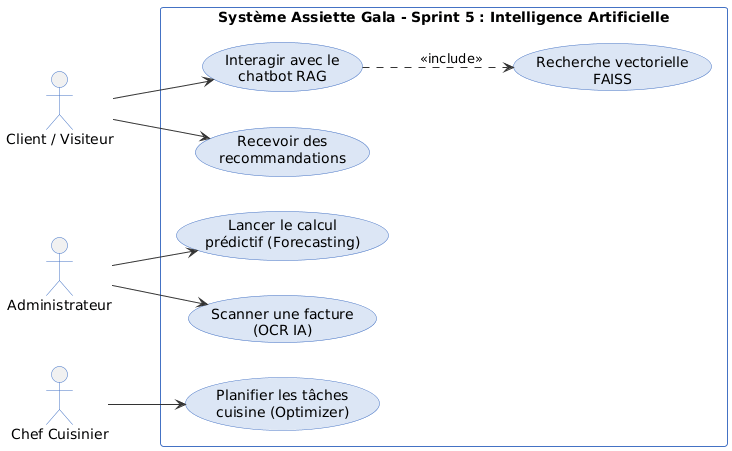
\includegraphics[width=0.85\textwidth]{uc_sprint5.png}
    \caption{Diagramme de cas d'utilisation : Intelligence Artificielle}
    \label{fig:uc_sprint5_ia}
\end{figure}

\subsection{Diagramme de classes}

\begin{figure}[H]
    \centering
    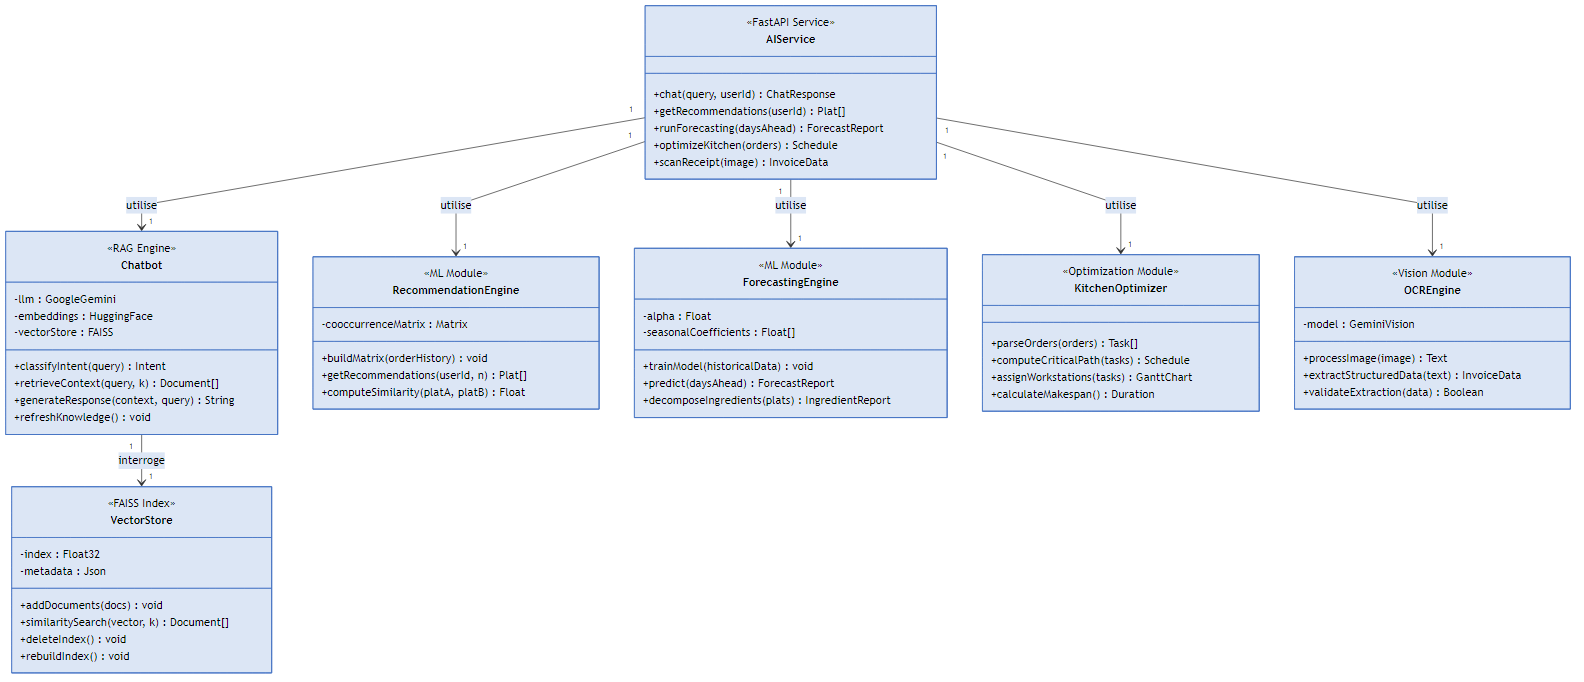
\includegraphics[width=0.95\textwidth]{class_sprint5.png}
    \caption{Diagramme de classes du sprint 5 : Modules IA}
    \label{fig:class_sprint5}
\end{figure}

\subsection{Diagramme d'états-transitions du chatbot}

\begin{figure}[H]
    \centering
    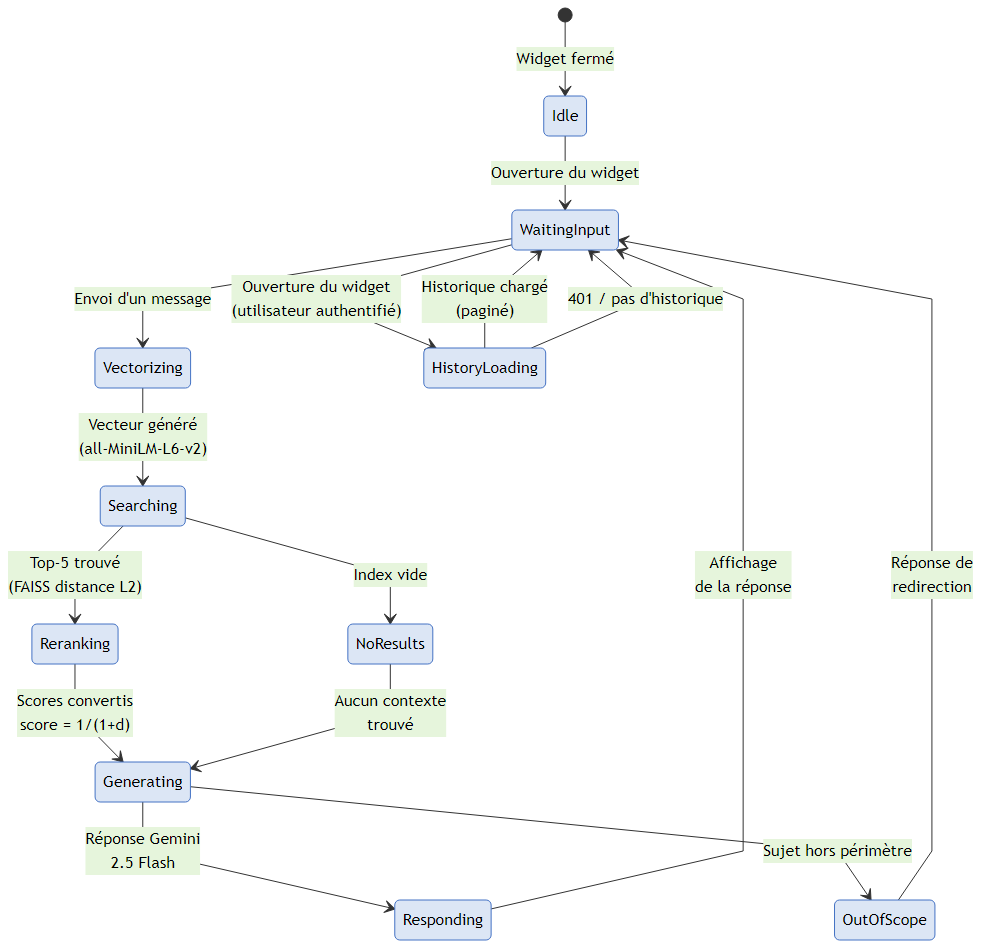
\includegraphics[width=0.85\textwidth]{state_sprint5_chatbot.png}
    \caption{Diagramme d'états-transitions : Conversation chatbot}
    \label{fig:state_chatbot}
\end{figure}

\subsection{Description textuelle : Interagir avec le chatbot}

\begin{table}[H]
    \centering
    \caption{Description textuelle : Interaction chatbot}
    \label{tab:desc_chatbot}
    \renewcommand{\arraystretch}{1.3}
    \begin{tabular}{|p{4cm}|p{8.5cm}|}
        \hline
        \textbf{Cas d'utilisation} & Interagir avec le chatbot RAG \\
        \hline
        \textbf{Acteur principal} & Client / Visiteur \\
        \hline
        \textbf{Précondition} & Accès à l'interface web \\
        \hline
        \textbf{Postcondition} & Réponse générée affichée \\
        \hline
        \textbf{Scénario principal} &
        \begin{enumerate}
            \item L'utilisateur pose une question dans le widget
            \item Vectorisation via \textit{all-MiniLM-L6-v2}
            \item FAISS extrait le contexte du catalogue
            \item Prompt envoyé à Gemini 2.5 Flash
            \item Réponse affichée
        \end{enumerate} \\
        \hline
    \end{tabular}
\end{table}

\subsection{Points d'entrée de l'API (FastAPI)}

\begin{table}[H]
    \centering
    \caption{Endpoints REST du microservice IA}
    \label{tab:endpoints_ia}
    \renewcommand{\arraystretch}{1.2}
    \begin{tabular}{|l|p{4.5cm}|p{5.5cm}|}
        \hline
        \textbf{Méthode} & \textbf{Route} & \textbf{Description} \\
        \hline
        POST & /api/chat/message & Envoi d'une question au chatbot \\
        \hline
        GET & /api/recommendations & Suggestions de plats \\
        \hline
        POST & /api/forecasting/run & Lancement du calcul prédictif des stocks \\
        \hline
        POST & /api/ocr/scan-receipt & Extraction de données de facture \\
        \hline
    \end{tabular}
\end{table}

\subsection{Tests fonctionnels}

\begin{table}[H]
    \centering
    \caption{Tests fonctionnels : Sprint 5}
    \label{tab:tests_sprint5}
    \renewcommand{\arraystretch}{1.3}
    \begin{tabular}{|c|p{4cm}|p{4cm}|p{2cm}|}
        \hline
        \textbf{N°} & \textbf{Cas de test} & \textbf{Comportement attendu} & \textbf{Résultat} \\
        \hline
        1 & Question complexe au chatbot & Réponse précise sans hallucination & Réussi \\
        \hline
        2 & Calcul Forecasting sur historique & Prédiction cohérente avec les tendances & Réussi \\
        \hline
        3 & Upload facture illisible (OCR) & Message d'erreur approprié & Réussi \\
        \hline
        4 & Ordonnancement cuisine & Pas de chevauchement de tâches sur un même four & Réussi \\
        \hline
    \end{tabular}
\end{table}

% --------------------------------------------------
\section*{Conclusion}
\addcontentsline{toc}{section}{Conclusion}

\begin{samepage}
Ce cinquième sprint clôture le cycle de développement en démontrant la capacité du projet à dépasser le stade de l'application web classique pour s'inscrire dans l'ère de l'intelligence artificielle appliquée. L'implémentation de modèles mathématiques de prévision, d'algorithmes d'optimisation de ressources et d'architectures RAG confère à cette plateforme une profondeur technique digne d'un diplôme de Master. Le système est désormais complet, de la sécurisation des accès à l'aide à la décision stratégique de haut niveau.
\end{samepage}



% Conclusion Générale
\clearpage
\renewcommand{\currentchapcolor}{black}
% ============================================================
% CONCLUSION GÉNÉRALE
% ============================================================
\chapter*{\centering Conclusion générale}
\addcontentsline{toc}{chapter}{Conclusion générale}
\markboth{Conclusion générale}{Conclusion générale}

Ce projet de fin d'études a permis de concevoir et de mettre en œuvre une plateforme web destinée à la digitalisation des activités de \textbf{Assiette Gala Sfaxienne}. Les objectifs fixés en introduction ont été globalement atteints: sécurisation des accès, gestion du catalogue, traitement des commandes, prise en charge des événements, pilotage par les données et intégration d'une assistance intelligente.

\section*{Bilan technique}

Sur le plan architectural, l'approche microservices, orchestrée par une API Gateway, a offert un cadre de développement structuré et modulaire. Cette organisation a facilité la séparation des responsabilités et l'évolution progressive des fonctionnalités.

Les technologies retenues ont répondu aux besoins du projet :
\begin{itemize}
    \item \textbf{Node.js/TypeScript} pour les services métier (authentification, catalogue, commandes, événements) et la passerelle API.
    \item \textbf{React/Vite} avec Tailwind CSS et Framer Motion pour une interface utilisateur réactive et professionnelle.
    \item \textbf{Python/FastAPI} pour le module d'intelligence artificielle (chatbot RAG et recommandations), avec un index vectoriel FAISS pour la recherche de similarité.
    \item \textbf{PostgreSQL/Prisma} pour la persistance et la structuration des données métier.
    \item \textbf{Recharts} pour les visualisations graphiques du tableau de bord décisionnel.
\end{itemize}

\section*{Résultats obtenus}

Le déroulement en cinq sprints a permis de livrer des résultats concrets et progressifs :
\begin{enumerate}
    \item \textbf{Sprint 1 (Gestion des utilisateurs)} : Infrastructure de sécurité avec JWT, Google OAuth 2.0, vérification par email et persistance de session.
    \item \textbf{Sprint 2 (Catalogue et Logistique)} : Vitrine culinaire avec gestion des plats, des allergènes, du stockage d'images Cloudinary, ainsi que le suivi des stocks et des fournisseurs.
    \item \textbf{Sprint 3 (Événements et Commandes)} : Tunnel de vente complet, panier d'achat, paiement à la livraison, et gestion des demandes de devis sur mesure pour les événements.
    \item \textbf{Sprint 4 (Back-Office et Analytics)} : Tableau de bord décisionnel (Recharts), pilotage des flux financiers (caisse et dépenses), et génération des documents comptables légaux (factures PDF).
    \item \textbf{Sprint 5 (Intelligence Artificielle)} : Intégration algorithmique de niveau Master avec un Chatbot RAG (FAISS/Gemini), un moteur de recommandation, l'IA Forecasting pour les stocks, le Kitchen Optimizer pour l'ordonnancement en cuisine, et l'AI Scanner (OCR) pour les factures.
\end{enumerate}

Les renforcements transverses incluent : limitation de débit (rate limiting), jeton de service interne pour les communications inter-services, Content-Security-Policy renforcée, arrêt gracieux des services (graceful shutdown), et centralisation des utilitaires dans le package partagé \texttt{@traiteurpro/shared}.

\section*{Limites et perspectives}

Malgré les résultats obtenus, certaines limites subsistent et ouvrent des axes d'amélioration :

\begin{itemize}
    \item Renforcement de l'observabilité (métriques, traces distribuées, journalisation centralisée).
    \item Augmentation de la couverture de tests automatisés (unitaires, intégration, end-to-end).
    \item Amélioration de la résilience inter-services (retries, circuit breaker, files d'attente).
    \item Déploiement cloud industrialisé (CI/CD, conteneurisation Docker, orchestration Kubernetes).
    \item Extension fonctionnelle via une application mobile native et des analytiques prédictives avancées.
    \item Intégration de passerelles de paiement en ligne supplémentaires (Flouci, D17) pour diversifier les modes de règlement.
\end{itemize}

\vspace{1cm}

En synthèse, ce travail a permis de proposer une solution cohérente, évolutive et orientée métier, répondant aux besoins actuels de l'entreprise. La combinaison d'une architecture microservices rigoureuse, d'une intelligence artificielle contextuelle et de modules de gestion professionnels constitue une base solide pour des évolutions futures, tant sur le plan fonctionnel que sur le plan technique.



% : Bibliographie ---
% ============================================================
% BIBLIOGRAPHIE
% ============================================================
\renewcommand{\currentchapcolor}{black}
\chapter*{Bibliographie}
\markboth{Bibliographie}{}
\addcontentsline{toc}{chapter}{Bibliographie}

\begin{enumerate}[label={[\arabic*]},series=refs]

    \item E. Gamma, R. Helm, R. Johnson et J. Vlissides, \textit{Design Patterns: Elements of Reusable Object-Oriented Software}, Addison-Wesley, 1994.

    \item S. Newman, \textit{Building Microservices: Designing Fine-Grained Systems}, 2nd Edition, O'Reilly Media, 2021.

    \item C. Richardson, \textit{Microservices Patterns: With Examples in Java}, Manning Publications, 2018.

    \item C. Aubry, \textit{Scrum : Pour une pratique vivante de l'agilité}, 5\textsuperscript{e} édition, Dunod, 2015.

    \item P. Lewis, E. Perez, A. Piktus et al., «\,Retrieval-Augmented Generation for Knowledge-Intensive NLP Tasks\,», \textit{Advances in Neural Information Processing Systems}, vol. 33, pp. 9459--9474, 2020.

    \item A. Vaswani, N. Shazeer, N. Parmar et al., «\,Attention Is All You Need\,», \textit{Advances in Neural Information Processing Systems}, vol. 30, 2017.

    \item Documentation officielle de Node.js : \url{https://nodejs.org/docs/latest/api/}

    \item Documentation officielle de React : \url{https://react.dev/}

    \item Documentation officielle de TypeScript : \url{https://www.typescriptlang.org/docs/}

    \item Documentation officielle Prisma ORM : \url{https://www.prisma.io/docs}

    \item Documentation officielle PostgreSQL : \url{https://www.postgresql.org/docs/}

    \item Documentation officielle Express.js : \url{https://expressjs.com/}

    \item Documentation officielle de LangChain : \url{https://python.langchain.com/docs/}

    \item Documentation officielle de Google Gemini API : \url{https://ai.google.dev/docs}

    \item Documentation Vite : \url{https://vite.dev/guide/}

    \item Documentation Tailwind CSS : \url{https://tailwindcss.com/docs}

    \item Documentation Cloudinary : \url{https://cloudinary.com/documentation}

    \item Documentation FAISS (Facebook AI Similarity Search) : \url{https://github.com/facebookresearch/faiss/wiki}

    \item Documentation officielle de Figma : \url{https://help.figma.com/}

    \item K. Schwaber, J. Sutherland, \textit{The Scrum Guide}, Scrum.org, 2020. Disponible sur : \url{https://scrumguides.org/}

    \item Documentation Recharts : \url{https://recharts.org/en-US/api}

\end{enumerate}

\vspace{1cm}

\chapter*{Webographie}
\markboth{Webographie}{}
\addcontentsline{toc}{chapter}{Webographie}

\begin{enumerate}[label={[\arabic*]},resume=refs]

    \item «\,Microservices Architecture\,», \textit{Microsoft Azure Architecture Center}, consulté le 15/02/2026. \url{https://learn.microsoft.com/en-us/azure/architecture/guide/architecture-styles/microservices}

    \item «\,API Gateway Pattern\,», \textit{Microservices.io}, consulté le 15/02/2026. \url{https://microservices.io/patterns/apigateway.html}

    \item «\,Introduction to RAG\,», \textit{Google Cloud}, consulté le 20/02/2026. \url{https://cloud.google.com/use-cases/retrieval-augmented-generation}

    \item «\,JWT Introduction\,», \textit{jwt.io}, consulté le 10/02/2026. \url{https://jwt.io/introduction}

    \item «\,Sentence Transformers Documentation\,», \textit{HuggingFace}, consulté le 12/03/2026. \url{https://huggingface.co/docs/sentence-transformers/}

    \item «\,Understanding UML Diagrams\,», \textit{Visual Paradigm}, consulté le 05/02/2026. \url{https://www.visual-paradigm.com/guide/uml-unified-modeling-language/}

    \item «\,Scrum Methodology\,», \textit{Atlassian}, consulté le 08/02/2026. \url{https://www.atlassian.com/agile/scrum}

    \item «\,PostgreSQL vs MySQL\,», \textit{DigitalOcean}, consulté le 10/02/2026. \url{https://www.digitalocean.com/community/tutorials/postgresql-vs-mysql}

\end{enumerate}


\end{document}
